\def\myfiledate{2021-03-29}

% zip manual *.tex *.bbl *.pdf

\documentclass[a4paper,twoside]{article}
\usepackage{ucs}\usepackage[utf8x]{inputenc}
\usepackage{natbib}
\usepackage{chem}
%\usepackage{afterpage}
\usepackage{dirtree}
\usepackage{url}
\usepackage{color}
%\usepackage{multicol}
\usepackage{rotating} % loads graphicx
%\usepackage{longtable}
\usepackage{graphicx}
%\usepackage{eclclass}
%\usepackage{verbatim}
%\usepackage{mypdfdraftcopy}\draftstring{DRAFT}\draftfontsize{150}\draftangle{60}
\usepackage[pdftex,bookmarks=false,colorlinks]{hyperref}
\hypersetup{anchorcolor=black,citecolor=black,filecolor=black,linkcolor=black,%
  menucolor=black,urlcolor=black}
\usepackage[shortlabels]{enumitem}\setlist[enumerate]{nosep}\setlist[itemize]{nosep}

% INDEX:
\usepackage{makeidx}\makeindex
\newcommand{\I}[1]{\index{#1}}
\newcommand{\IT}[1]{#1\index{#1}}
% activate next line for testing:
%\usepackage{showidx}\setlength{\marginparwidth}{3cm}\textwidth150mm\oddsidemargin-5mm\evensidemargin15mm\def\twocolumn{}

% activate to show "draft" watermark:
%\usepackage{pdfdraftcopy}\draftstring{DRAFT}\draftfontsize{150}\draftangle{60}

\oddsidemargin-5mm
\evensidemargin-5mm
\topmargin-15mm
\textheight260mm
\textwidth175mm
\raggedbottom
\parindent0mm
\parskip1.0ex plus0.5ex minus0.5ex
\renewcommand{\arraystretch}{1}
\renewcommand{\topfraction}{0.95}
\renewcommand{\dbltopfraction}{0.95}
\renewcommand{\bottomfraction}{0.95}
\renewcommand{\floatpagefraction}{0.9}
\renewcommand{\dblfloatpagefraction}{0.9}
\renewcommand{\textfraction}{0.1}
\setcounter{topnumber}{3}
\setcounter{bottomnumber}{3}

\newcommand{\todo}[1]{{\color{red}\uppercase{\bf ((#1))}}}
\newcommand{\egcite}[1]{\citep[e.g.][]{#1}}

\newcommand{\tophline}{\hline\noalign{\vspace{1mm}}}
\newcommand{\middlehline}{\noalign{\vspace{1mm}}\hline\noalign{\vspace{1mm}}}
\newcommand{\bottomhline}{\noalign{\vspace{1mm}}\hline}

\def\nosep{\setlength\parsep{0mm}\setlength\topsep{0mm}\setlength\itemsep{0mm}}
\setlength{\columnsep}{8mm}

\def\mypageheader{Sander et al.: CAABA/MECCA User Manual}
\markboth{\mypageheader}{\mypageheader}
\pagestyle{myheadings}

% created automatically by xmecca, DO NOT EDIT!
% xmecca was run on 2023-09-13 at 15:50:31 by user taras on machine taras
\def\meccaversion{\code{4.4.2}}
\def\kppversion{\code{2.2.3_rs3}}
\def\gaseqnfile{\code{gas.eqn}}
\def\wanted{\code{Tr and (G or (Aa or Mbl)) and not I and not Hg}}
\def\inifile{\code{example.ini}}
\def\integr{\code{rosenbrock_posdef}}
\def\rplfile{\code{}}
\def\apn{1}
\def\gasspc{671}
\def\aqspc{462}
\def\allspc{1133}
\def\Geqns{1741}
\def\Aeqns{385}
\def\Heqns{713}
\def\Jeqns{348}
\def\PHeqns{26}
\def\HETeqns{0}
\def\EQeqns{112}
\def\IEXeqns{0}
\def\TAGeqns{0}
\def\Deqns{1}
\def\alleqns{3326}
 % \def\meccaversion{...}

% line break after \paragraph:
\makeatletter
\renewcommand\paragraph{\@startsection{paragraph}{4}{\z@}%
  {-2.0ex\@plus -1ex \@minus -.2ex}%
  {1.0ex \@plus .2ex}%
  {\normalfont\normalsize\bfseries}}
\makeatother
% \paragraph should also be numbered
\setcounter{secnumdepth}{4}

\I{SZA|see{solar zenith angle}}
\I{$\alpha$|see{accommodation coefficient}}
\I{APN|see{aerosol phase number}}
\I{awk|see{gawk}}
\I{make|see{gmake}}
\I{ampersand|see{{\tt \&}}}
\I{dollar sign|see{{\tt \$}}}
\I{dry deposition|see{deposition}}
\I{ODE|see{ordinary differential equation}}
\I{EMAC|see{ECHAM5/MESSy}}
\I{curly braces|see{$\{\}$}}
\I{LWC|see{liquid water content}}
\I{angle brackets|see{\textless\textgreater}}
\I{MCM|see{master chemical mechanism}}
\I{nml|see{namelist}}
\I{K|see{Kelvin}}
\I{Pa|see{Pascal}}
\I{KPP|see{Kinetic PreProcessor}}
\I{rpl|see{replacement file}}
\I{spc|see{species file}}
\I{eqn|see{equation file}}
\I{JVPP|see{JVAL PreProcessor}}
%\I{|see{}}

\begin{document}

\thispagestyle{empty}
\begin{center}
  \vspace*{-15mm}
  
\includegraphics[height=0.3\textheight]{caaba_mecca_logo_print}\\[10mm]
  {\Huge\bf CAABA/MECCA-{\meccaversion}}\\[5mm]
  {\Huge\bf User Manual}\\[10mm]
  {\huge\em \underline{C}hemistry \underline{A}s \underline{A}
    \underline{B}oxmodel \underline{A}pplication /}\\[3mm]
  {\huge\em \underline{M}odule \underline{E}fficiently
    \underline{C}alculating the\\[5mm]
    \underline{C}hemistry of the
    \underline{A}tmosphere}\\[5mm]
  {\huge\bf Rolf Sander$^1$ et al.$^2$}\\[5mm]
  \Large
  Air Chemistry Department\\
  Max-Planck Institute of Chemistry\\
  PO Box 3060, 55020 Mainz, Germany\\
  \url{rolf.sander@mpic.de}\\[5mm]
  $^1$self-appointed BDFL\\ 
  $^2$with many contributions from
  A.~Baumgaertner,
  T.~Butler,
  D.~Cabrera-Perez,
  F.~Frank,
  K.-D.~Gottschaldt,
  S.~Gromov,
  J.-U.~Groo\ss,
  H.~Harder,
  K.~Hens,
  V.~Huijnen,
  P.~J\"ockel,
  V.~A.~Karydis,
  A.~Kerkweg,
  F.~K\"ollner,
  D.~Kubistin,
  K.~E.~Niemeyer,
  A.~Pozzer,
  E.~Regelin,
  H.~Riede,
  A.~Sandu,
  M.~Schultz,
  D.~Taraborrelli,
  S.~Tauer,
  H.~Tost and
  Z.-Q.~Xie\\[5mm]

  {\huge\url{http://www.mecca.messy-interface.org}}

  \vfill

  % see also IfFileExists in meccanism.tex:
  \IfFileExists{/home/sander/papers/sander-caaba4-refxxxx/README}
  {{\large This manual is part of the electronic supplement of our
      article ``The atmospheric chemistry box model CAABA/MECCA-4.0'' in
      Geosci.\ Model Dev.\ (2017???), available at:
      \url{http://www.geosci-model-dev.net}}} % if branch
  {} % else branch

  Date: \myfiledate

\end{center}

\clearpage

\setlength{\columnsep}{8mm}
\twocolumn\sloppy

\tableofcontents

\clearpage

\begin{figure*}%[htb]
  \begin{center}
  \includegraphics[width=0.9\textwidth]{modular-mecca}
  \end{center}
  \caption{Diagram showing \IT{MECCA} as part of the
    \IT{CAABA} \IT{box model} or of a global model.}
  \label{fig:modular-mecca}
\end{figure*}

\section{Introduction}

\IT{MECCA} (\underline{M}odule \underline{E}fficiently
\underline{C}alculating the \underline{C}hemistry of the
\underline{A}tmosphere) is an atmospheric \IT{chemistry} module that
contains a comprehensive chemical \IT{reaction mechanism} with
\I{troposphere}tropospheric and \I{stratosphere}stratospheric chemistry
of both, the gas and the \IT{aqueous phase} \citep{1666,2405,3264}. For
the numerical integration, MECCA uses the \I{Kinetic PreProcessor}KPP
software \citep{1665}.

To apply the \IT{chemistry} mechanism to atmospheric conditions, MECCA
must be connected to a \IT{base model}. As shown in
Fig.~\ref{fig:modular-mecca}, the base model can be a complex,
3-dimensional model but it can also be a simple \IT{box model}. This
manual focuses on MECCA (and other submodels) connected to the box model
\IT{CAABA} (\underline{C}hemistry \underline{A}s \underline{A}
\underline{B}oxmodel \underline{A}pplication). This combination will be
referred to as ``CAABA/MECCA''. The main features of the \IT{CAABA} box
model are shown in Fig.~\ref{fig:caaba_sketch}.

Section~\ref{sec:messy} describes the connection of MECCA to other base
models (e.g., the 3-dimensional GCM ECHAM5/MESSy) via the \IT{MESSy}
interface.

\section{Installation}
\label{sec:install}

Arguably the easiest way to install the CAABA/MECCA system is to run it
inside a \IT{virtual machine} as described in Sect.~\ref{sec:vm}. To
install CAABA/MECCA directly on your computer, follow the instructions
in Sections \ref{sec:systemrequirements}-\ref{sec:troubleshooting}. This
section can be skipped if CAABA/MECCA is already installed on your
computer.

\subsection{\I{virtual machine}Virtual machine}
\label{sec:vm}

\subsubsection{Installation}

CAABA/MECCA can be run in a virtual machine using either the VMware
(\url{http://downloads.vmware.com}) or the virtual box
(\url{https://www.virtualbox.org}) software. Here, we only describe how
to use VMware. Download the newest version of the ``VMware Workstation
Player'' from \url{https://my.vmware.com/web/vmware/downloads}. Next,
download all files from the directory
\url{https://owncloud.gwdg.de/index.php/s/Y3DrdXPSHceMWag} ($\approx$ 17
GB). Start the VMware Player and open the virtual machine
\verb|mint-18-caaba-4.0.vmx|. When asked ``copy or move?'', it is
recommended to answer ``copy''. This will generate a new MAC address for
the virtual machine and avoid potential problems of duplicate MAC and IP
addresses. After booting the virtual machine, enter the User-ID
\verb|caaba| and the initial password for the CAABA/MECCA-4 virtual
machine (\verb|CaMe4ViMa|). It is strongly suggested to change the
password as soon as possible in the ``System $\rightarrow$
Administration $\rightarrow$ Users and Groups'' menu.

\subsubsection{Virtual machine settings}

\begin{description}
\item[Memory:] {\em $\geq$ 2 GB.} Less memory would cause potential trouble
  with the KPP software that is needed by MECCA.
\item[Processors:] {\em 1 CPU.} More than 1 would not speed up the model
  significantly.
\item[Harddisk:] {\em SCSI, 20 GB maximum size, not preallocated, single
    file.}
\item[CD/DVD:] {\em SATA, not connected.}
\item[Network Adapter:] {\em Connected at power on, NAT.} The setting
  ``NAT'' is highly recommended. It is best for using the virtual
  machine only on the host computer and safer to operate (regarding
  IP/MAC collisions/firewall, services, \dots). In contrast, with the
  setting ``Bridged'', the machine is directly connected to the local
  network with its own IP address and easy external access. If you do
  choose ``Bridged'', it is strongly recommended to change the password
  because the machine is visible externally. Also, system updates to
  prevent hacks should be made and care needs to be taken for the
  initial setup, making sure to use a different MAC address and hostname
  for DHCP.
\item[USB controller:] {\em Auto connect, enable USB 2.0 devices.}
  Easier to deal with USB sticks for ``take away files''.
\item[Display:] {\em Auto detect.}
\item[Shared folders:] {\em Enabled.} Shared folders are initially
  disabled. Set to ``Always enabled'' and define a suitable ``host
  path''. Then, files in the ``stargate'' directory on the desktop of
  the virtual machine are syncronized with the ``host path'' directory
  on your (real) machine. This can be used for file transfer between the
  virtual machine and the host.
\end{description}

\subsubsection{Troubleshooting}

\begin{itemize}
\item If VMware complains about a version mismatch, it may help to
  change the value of \verb|virtualHW.version = "12"| in the *.vmx file.
\item The virtual machine uses a German keyboard layout. If you have a
  different keyboard, you have to change the settings, e.g.: System
  $\rightarrow$ Preferences $\rightarrow$ Hardware $\rightarrow$
  Keyboard $\rightarrow$ Layouts $\rightarrow$ Add $\rightarrow$
  Country: United States, Variants: USA.
\item If there is no internet connection, it may be necessary to
  ``Enable networking'' by clicking on the network icon in the bottom
  panel.
\end{itemize}

\subsection{System Requirements}
\label{sec:systemrequirements}

\subsubsection{\IT{Linux}/Unix}

\IT{CAABA/MECCA} has been tested successfully on several \IT{UNIX}-like
operating systems. On a \IT{Linux} PC, many of the auxiliary programs
described in Sect.~\ref{sec:prerequisites} are already included in a
typical distribution.

\subsubsection{\IT{MAC} OS X}

\IT{CAABA/MECCA} does not work with the version of the \I{sed}\verb|sed|
program that is shipped with MAC OS X. Instead, it is necessary to
install the \IT{GNU} version of \verb|sed|, called \verb|gsed|. This can
be done using the MacPorts (\url{http://www.macports.org/}). To ensure
that \verb|gsed| is always executed when \verb|sed| is called, a
symbolic link from \verb|sed| to \verb|gsed| can be created, e.g.:
\begin{verbatim}
sudo ln -s /opt/local/bin/gsed
  /opt/local/bin/sed
\end{verbatim}
\I{sudo}Also, there may be problems executing the command
``\verb|echo -n|'' under OS X. If this is the case, the script
\I{xmecca}\verb|xmecca| needs to be adjusted.

\subsubsection{\IT{Windows}}

A native installation under \IT{Windows} is neither recommended nor
supported. However, it is possible to execute the model in a virtual
machine running \IT{Linux} on a \IT{Windows} PC as described above
(Sect.~\ref{sec:vm}).

\begin{figure*}%[htb]
  \begin{center}
  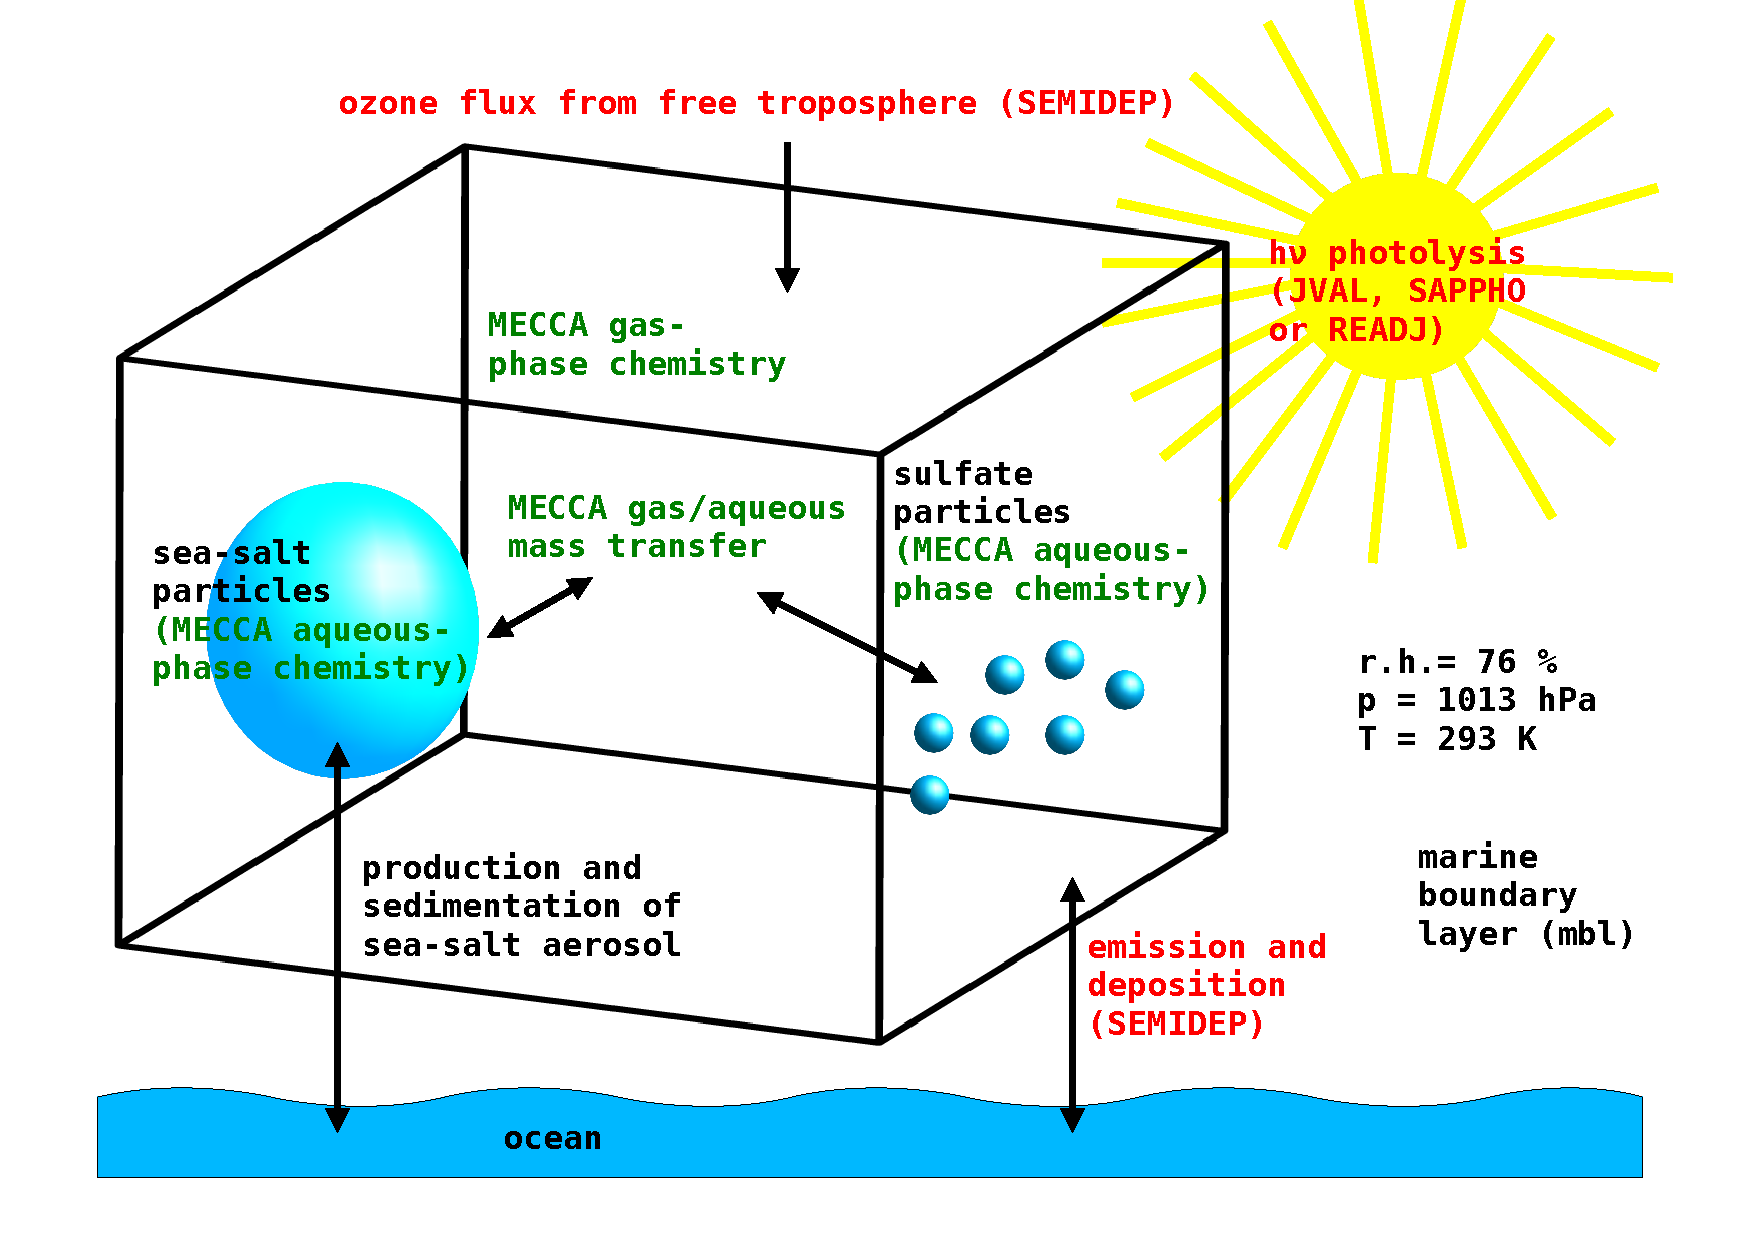
\includegraphics[width=0.9\textwidth]{caaba_sketch}
  \end{center}
  \caption{The \IT{CAABA} \IT{box model}}
  \label{fig:caaba_sketch}
\end{figure*}

\subsection{Prerequisites}
\label{sec:prerequisites}

\begin{description}
\item[A \IT{Fortran95} \IT{compiler} (mandatory):] Several compilers
  have been tested successfully: \IT{g95} (for \IT{Linux}),
  \IT{Lahey}/\IT{Fujitsu} (for \IT{Linux}), \IT{Intel} (for \IT{Linux}),
  Compaq (\I{Alpha (Compaq)}Alpha \IT{UNIX}). Other compilers can be
  used as well, if they accept standard Fortran95 code. It should be
  noted that the g95 compiler for \IT{Linux} is free and can be
  downloaded from \url{http://www.g95.org/}.
\item[The Kinetic PreProcessor \I{Kinetic PreProcessor}KPP (mandatory):]
  This flexible numerical integration package by \citet{1665} transforms
  the chemical \IT{reaction mechanism} into a set of \IT{ordinary
    differential equation}s (ODEs) in Fortran95 syntax. \IT{MECCA} needs
  the \I{Kinetic PreProcessor}KPP version that is provided in the
  \verb|mecca/kpp/| directory. The CAABA/MECCA distribution already
  contains the linux executable file \verb|mecca/kpp/bin/kpp|. If it
  cannot be used on your machine, you have to compile KPP yourself,
  following the instructions in \verb|mecca/kpp/readme|.
\item[\I{python}Python (mandatory):] Version 3.6 of python plus several
  packages are needed. The \I{matplotlib}Matplotlib library is needed
  for plotting model results (see Sect.~\ref{sec:matplotlib} for
  details). Missing python packages can be installed with
  pip, e.g.:\\
  \verb|pip3 install f90nml|
\item[\IT{tcsh}, \IT{gawk}, sed, and \IT{gmake} (mandatory):] These
  \IT{UNIX} tools are standard on \IT{Linux} systems. Check that recent
  versions of them are installed. Especially gawk may lead to strange
  error
  messages. To test gawk, type:\\
  \verb|gawk 'BEGIN {print match("X","[^a-z]")}'|\\
  The result should be ``1''. However, you may get ``0'' as the result
  on your system. Supposedly, this is not a bug in gawk but a feature.
  You can solve the problem by setting the environment variable
  \verb|LC_ALL| to ``\verb|C|'':\\
  \verb|export LC_ALL=C| $\qquad$ (if you use \IT{bash})\\
  \verb|setenv LC_ALL C| $\qquad$ (if you use \IT{tcsh})\\
  When you try the gawk test again, it should work fine.
\item[La\TeX\ (optional):] If you have La\TeX\ installed on your
  computer, you can print a table (including rate coefficients and
  references) of the currently selected \IT{reaction mechanism} (see
  Sect.~\ref{sec:latextable} for details).
\item[\IT{netCDF} library (strongly recommended):] The netCDF library is
  needed to create model output in netCDF format. It can be obtained
  from \url{http://www.unidata.ucar.edu/software/netcdf/}. Note that the
  \verb|*.mod| files in the netCDF library are \IT{compiler}-specific.
  Thus, it is necessary to create a netCDF library for each
  \IT{Fortran95} compiler and maybe also for each Fortran95 compiler
  version.

  Software for manipulating or displaying \IT{netCDF} data is listed at:
  \url{http://www.unidata.ucar.edu/software/netcdf/software.html}. If
  you don't have the netCDF library, you can still run the model but
  produce only \IT{ASCII} output.
\item[\I{ferret}Ferret (optional):] The ferret plotting program
  (\url{http://ferret.wrc.noaa.gov/Ferret}) can be used to plot the
  contents of the \IT{netCDF} output using the scripts in the
  \verb|jnl/| directory (see Sect.~\ref{sec:ferret} for details). To
  ensure that ferret finds all necessary files, you have to add
  ``\verb|./tools|'' to the \I{FER\_GO}\verb|FER_GO| environment
  variable. For example, when using the \IT{tcsh}, type:\\
  \verb|setenv FER_GO "$FER_GO ./tools"|\\
  In addition, it must be ensured that the scripts \verb|plt2pdf| and
  \verb|double_line_widths| in the \verb|tools/| directory can be found.
  This can for example be done by copying these files to
  \verb|/usr/local/bin/| or by adding the \verb|tools/| directory to the
  \verb|$PATH|.
\item[\I{graph-tool}Graph-tool and \IT{graphviz} (optional):] These
  programs (\url{https://graph-tool.skewed.de} and
  \url{https://www.graphviz.org}) are needed to visualize chemical
  reaction schemes as graphs.
\item[\IT{fpc} \I{Pascal>programming language}Pascal \IT{compiler}
  (optional):] To use the \IT{tagging} diagnostics and \IT{isotope}
  modeling features (see Sect.~\ref{sec:tag} for details), version 2.6.0
  or higher of the free pascal compiler \verb|fpc| from
  \url{http://www.freepascal.org/} is needed.
\end{description}

\subsection{CAABA/MECCA code installation}

Once all prerequisites are fulfilled, you can install \IT{CAABA/MECCA}
by simply unpacking the zip archive:\\[2mm]
\I{unzip}{\tt unzip caaba\_\meccaversion.zip}\\[2mm]

Next, you have to check that all settings in \verb|Makefile| are
correct. If necessary, edit the file: Choose a \IT{Fortran95}
\IT{compiler} (\verb|COMPILER|), enter its name (\verb|F90|) and the
compiler options (\I{F90FLAGS}\verb|F90FLAGS|). If you add a new
compiler, check if you need to activate the \IT{C-preprocessor}
(\IT{CPP}) option. To activate \IT{netCDF} output, you also have to edit
the \verb|Makefile|:
\begin{itemize}
\item Check that the variable \verb|OUTPUT| is set to \verb|NETCDF| (not
  to \I{ASCII}\verb|ASCII|).
\item Enter the correct \IT{netCDF} library information in
  \verb|NETCDF_INCLUDE| and \verb|NETCDF_LIB|.
\end{itemize}

\subsection{Troubleshooting}
\label{sec:troubleshooting}

Should there be any problems with the \IT{CAABA/MECCA} installation,
please check the following:
\begin{itemize}
\item Confirm that all prerequisites (see above) are fulfilled!
\item Confirm that the \IT{tcsh} path in the first line of
  \I{xmecca}\verb|xmecca| is correct.
\item Confirm that the model code was \IT{unzip}ped successfully from
  the zip archive. Check for potential problems during the
  \IT{unzip}ping process:
  \begin{itemize}
  \item Do not unzip {\tt caaba\_\meccaversion.zip} under Windows! If
    you use a virtual machine (VM) under Windows, transfer the zip file
    to the VM first, and then unzip it inside the VM.
  \item Make sure that the directory structure has not changed.
    Unfortunately, some \IT{unzip}ping programs seem to put all files
    into one directory, ignoring the original directory structure.
  \item Make sure that links have not been converted to files. For
    example, the output of the command ``\verb|file caaba.nml|'' should
    tell you that \verb|caaba.nml| is a symbolic link to
    \verb|nml/simple/caaba.nml|.
  \end{itemize}
\end{itemize}

\section{Compiling and running the \IT{CAABA/MECCA} \IT{box model} with
  the \IT{python} script \I{xcaaba}{\tt xcaaba.py}}
\label{sec:xcaaba.py}

Open a terminal and go to the \IT{base directory} of the model code
(note that all path names given in this manual are relative to this
base directory):\\[2mm]
{\tt cd caaba\_\meccaversion}\\[2mm]
Next, the \IT{python} script \I{xcaaba}\verb|xcaaba.py| will guide you
through the process of running the box model, as illustrated in
Fig.~\ref{fig:flowcontrol_xcaaba}. To execute \verb|xcaaba.py|, type:
\begin{verbatim}
./xcaaba.py
\end{verbatim}
\I{xcaaba}\verb|xcaaba.py| will ask several questions, and recommended
answers are given below. If you only press the Return key, you select
the default.
\begin{verbatim}
Start xmecca?
\end{verbatim}
If you answer ``\verb|y|'', you can create a new chemical \IT{reaction
  mechanism} with \I{xmecca}\verb|xmecca| as described in detail in
Sect.~\ref{sec:xmecca}. However, for the first tests with
\IT{CAABA/MECCA} it is recommended to answer ``\verb|n|'' and use the
simple default mechanism.
\begin{verbatim}
Choose an option:
s = Start from scratch
c = Compile
r = Run existing executable
h = Help
q = Quit
\end{verbatim}
Choose ``\verb|c|'' to compile the \IT{Fortran95} code. After a
successful compilation, \I{xcaaba}\verb|xcaaba.py| asks you to choose a
\IT{namelist} file:
\begin{verbatim}
Choose a namelist file from
the nml/ directory:
...
\end{verbatim}
\I{namelist}Namelists control the behaviour of \IT{CAABA/MECCA} during
runtime, and editing them allows to define the model setup at runtime
(see Sect.~\ref{sec:nmlfiles}). The default is to use the same
\IT{namelist} as last time. For the first tests, the file
\verb|caaba_simple.nml| can be chosen. The active contents of the chosen
\IT{namelist} will be shown.

Finally, \I{xcaaba}\verb|xcaaba.py| asks if you want to run the model:
\begin{verbatim}
Run CAABA/MECCA?
y = yes (default)
m = multirun
n = no
q = quit
\end{verbatim}
Answer ``\verb|y|'', and the \IT{CAABA/MECCA} model simulation will
start. The flow control is illustrated in
Fig.~\ref{fig:caaba_flowcontrol}. The model day and the current
\IT{solar zenith angle} (sza) are printed on the screen during the model
simulation. The default is to integrate 8 days, unless a different value
is defined in the namelist.
\begin{verbatim}
Save the output and model code
in output/ directory?
\end{verbatim}
Answer ``\verb|y|'', and \I{xcaaba}\verb|xcaaba.py| will put the files
into a subdirectory with a name based on the date and \IT{time} of the
model simulation, e.g., \verb|output/2019-03-14-12:43:35/|. It is
recommended to rename the subdirectory to a more descriptive name.

Instead of answering all questions interactively, it is also possible to
run the model in batch mode by reading the input from a config file
(\verb|*.ini|) in the \verb|ini/| directory. Provide the \verb|*.ini|
file as a command line parameter with the \verb|-i| option, e.g.:
\begin{verbatim}
 ./xcaaba.py -i caaba_example.ini
\end{verbatim}
More information is available in the comments in
\verb|ini/caaba_example.ini|.

\section{Selecting a chemical \IT{reaction mechanism} with the
  shell script \I{xmecca}{\tt xmecca}}
\label{sec:xmecca}

\IT{MECCA} contains a very comprehensive set of chemical reactions in
both, the gas phase and the \IT{aqueous phase}. For many applications,
using the complete mechanism will consume too much \IT{CPU} time.
Therefore, the shell script \I{xmecca}\verb|xmecca| has been written
which allows to create a custom-made subset of the reaction mechanism
interactively. Normally, \I{xmecca}\verb|xmecca| is called via
\I{xcaaba}\verb|xcaaba.py|. However, you can also start it manually:
\begin{verbatim}
cd mecca
./xmecca
\end{verbatim}
\I{xmecca}\verb|xmecca| will ask several questions, and recommended
answers are given below. If you only press the Return key, you select
the default.
\begin{verbatim}
Select a batch file which defines
the chemistry mechanism that you
want to generate.
\end{verbatim}
It is strongly recommended that you select a \IT{batch file} here. Batch
files contain all the information that \I{xmecca}\verb|xmecca| needs to
create a chemical \IT{reaction mechanism}. Several batch files are
available already, and it is also possible to add your own batch files
as explained at the end of this section. If you do not select a valid
batch file, you can continue and answer all questions interactively as
described here.
\begin{verbatim}
How many aerosol phases?
\end{verbatim}
For a \I{gas phase}gas-phase only mechanism, type ``0''. For a mechanism
with \I{aqueous phase}aqueous-phase \IT{chemistry} in \IT{sea salt} and
in sulfate \IT{particle}s, type ``2''. Other values are possible if they
have been defined in subroutine \verb|define_aerosol| in
\verb|messy_mecca_box.f90|.
\begin{verbatim}
Available gas phase equation files:
1) gas.eqn
2) ...
3) ...
Type the number of a gas phase equation file:
\end{verbatim}
Answer ``1'' for the current MECCA chemistry. Other options allow to
select different chemical mechanisms (see Sect.~\ref{sec:othereqn}).

\begin{figure*}
  \begin{center}
    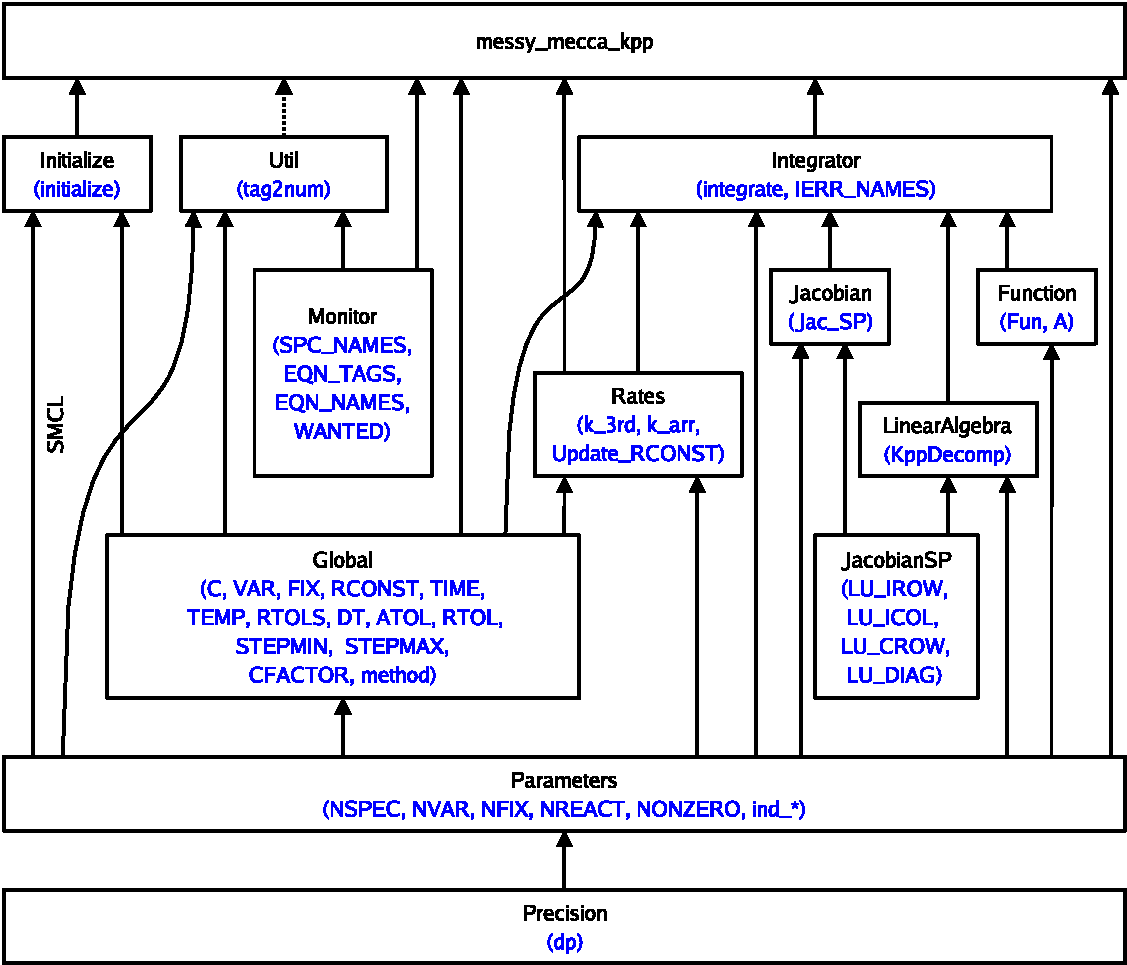
\includegraphics[width=\textwidth]{kpp_use_diagr}
  \end{center}
  \caption{Module structure of \I{Kinetic PreProcessor}KPP-produced
    \IT{Fortran95} files. The arrows start at the module which is
    exporting the {\tt PUBLIC} variables and subroutines (which are
    shown in blue). They point to the module importing them via the
    Fortran95 USE instruction. A dotted line represents an optional
    connection.}
  \label{fig:kpp_use_diagr}
\end{figure*}

\begin{verbatim}
Replacement files allow you to modify...
...
Do you want to modify gas.eqn?
\end{verbatim}
Answer ``0'' (``no replacements'') unless you want to apply a
\IT{replacement file}. More information about the replacement feature
can be found in the file \verb|rpl/gas.rpl-example|.
\begin{verbatim}
Type the number of your selection or
type a boolean expression:
\end{verbatim}
\I{boolean expression}Now you can choose a subset of the chemical
\IT{reaction mechanism}. A few predefined standard selections are
available. For all other purposes, a \IT{batch file} should be created,
as explained at the end of this section. Some of the predefined
selections are:
\begin{description}
\item [\IT{EVAL}:] A selection that was used for the evaluation of the
  \IT{MECCA} \IT{chemistry} in the global model \IT{ECHAM5/MESSy}
  \citep{1851}.
\item [Minimum \I{troposphere}tropospheric \IT{chemistry}:] A
  very small tropospheric mechanism.
\item [Minimum \IT{MBL} \IT{chemistry}:] A small mechanism
  that contains \I{aqueous phase}aqueous-phase chemistry and should
  only be used if the number of \IT{aerosol} phases is $>0$.
\end{description}
To define a set of chemical reactions, you can either type the number of
a pre-defined selection or enter a boolean expression based on the
\IT{label}s, as described in Sect.~\ref{sec:markerslabels}.
\begin{verbatim}
Activate enthalpy (kJ/mol) in
equation file?
\end{verbatim}
\I{enthalpy}Answer ``\verb|n|'' here unless you want to calculate
the reaction enthalpies. This is only useful for the upper atmosphere.
\begin{verbatim}
Add Monte-Carlo factor to all rate
coefficients?
\end{verbatim}
Answer ``\verb|n|'' here unless you want to perform Monte-Carlo
calculations, as described in Sect.~\ref{sec:montecarlo}.
\begin{verbatim}
Add diagnostic tracers to gas.eqn?
[q/0/?, default=0]
\end{verbatim}
Answer ``0''. Diagnostic \IT{tracer}s are usually only used for
3-dimensional model simulations.
\begin{verbatim}
Calculate accumulated reaction rates
of all equations?
\end{verbatim}
Answer ``\verb|y|'' if you want to have all accumulated
\IT{reaction rate}s in the model output. Otherwise, answer
``\verb|n|''.
\begin{verbatim}
Perform mechanism (isotope) tagging?
\end{verbatim}
If you want to activate \IT{tagging} diagnostics and \IT{isotope}
modeling, please read Sect.~\ref{sec:tag} first. Otherwise, answer
``\verb|n|''.
\begin{verbatim}
Run KPP?
\end{verbatim}
Answer ``\verb|y|''.
\begin{verbatim}
Type the number of an integrator:
\end{verbatim}
Several numerical integrators are defined in the subdirectory
\verb|mecca/kpp/int/| and can be used with \I{Kinetic PreProcessor}KPP.
The default is the \IT{positive definite} \IT{Rosenbrock solver} with
automatic time-step control (\verb|rosenbrock_posdef|). It is very
robust and capable of integrating very \IT{stiff sets of equations}
(e.g., chemical \IT{reaction mechanism}s including both, gas- and
\I{aqueous phase}aqueous-phase \IT{chemistry}). Although a
\IT{Rosenbrock solver} with manual time-step control
(\verb|ros2_manual|) is also available, it is strongly recommended not
to use it for stiff sets of equations. If you choose it, you do so at
your own risk! Next, \I{Kinetic PreProcessor}KPP will create several
\IT{Fortran95} files.
\begin{verbatim}
Remove indirect indexing with decomp?
\end{verbatim}
If this question shows up, answer ``\verb|n|''.
\begin{verbatim}
Create LaTeX listing of selected mechanism?
[y/n/q, default=n]
\end{verbatim}
\I{LaTeX}If you answer ``\verb|y|'' here, a table of the current
\IT{reaction mechanism} will be produced. Only the selected reactions
will be listed. The table also contains the rate coefficients and their
references, as described in Sect.~\ref{sec:latextable}.
\begin{verbatim}
Create graphviz plots of selected
mechanism?
\end{verbatim}
If you have the ``\verb|dot|'' program from the \IT{graphviz} software
installed, you can create graphical visualizations of the \IT{reaction
  mechanism}, see Sect.~\ref{sec:graphviz} for details.
\begin{verbatim}
Do you want to delete the temporary
xmecca files?
\end{verbatim}
It is okay to delete these temporary files unless you need them for
debugging purposes.

When \I{xmecca}\verb|xmecca| finishes successfully, the \IT{Fortran95}
code of your selected \IT{reaction mechanism} has been created. The
\I{Kinetic PreProcessor}KPP-produced Fortran95 files
(Tab.~\ref{tab:files}) are moved into the \verb|mecca/smcl/| directory
(with lower-case names). An exception is
\verb|messy_mecca_kpp_Model.f90|, which is produced by \I{Kinetic
  PreProcessor}KPP but not needed for \IT{MECCA}. The modular structure
of the \I{Kinetic PreProcessor}KPP-produced Fortran95 files is shown in
Fig.~\ref{fig:kpp_use_diagr}.

If you need to create a \IT{reaction mechanism} very often, it is quite
tedious to answer all questions every time. To make this easier, you can
copy the template \verb|batch/example.bat| to a new name (containing only
alphanumeric characters, ``-'', ``\_'', and ``.'', e.g.,
\verb|batch/myfile.bat|) and then enter your answers into that
\IT{batch file}. Now you can create a new mechanism in batch mode with
\begin{verbatim}
./xmecca myfile
\end{verbatim}
To add the name of the batch file to the \I{xcaaba}\verb|xcaaba.py|
command, use the \verb|-b| option:
\begin{verbatim}
./xcaaba.py -b myfile
\end{verbatim}

\begin{figure*}%[htb]
  \begin{center}
  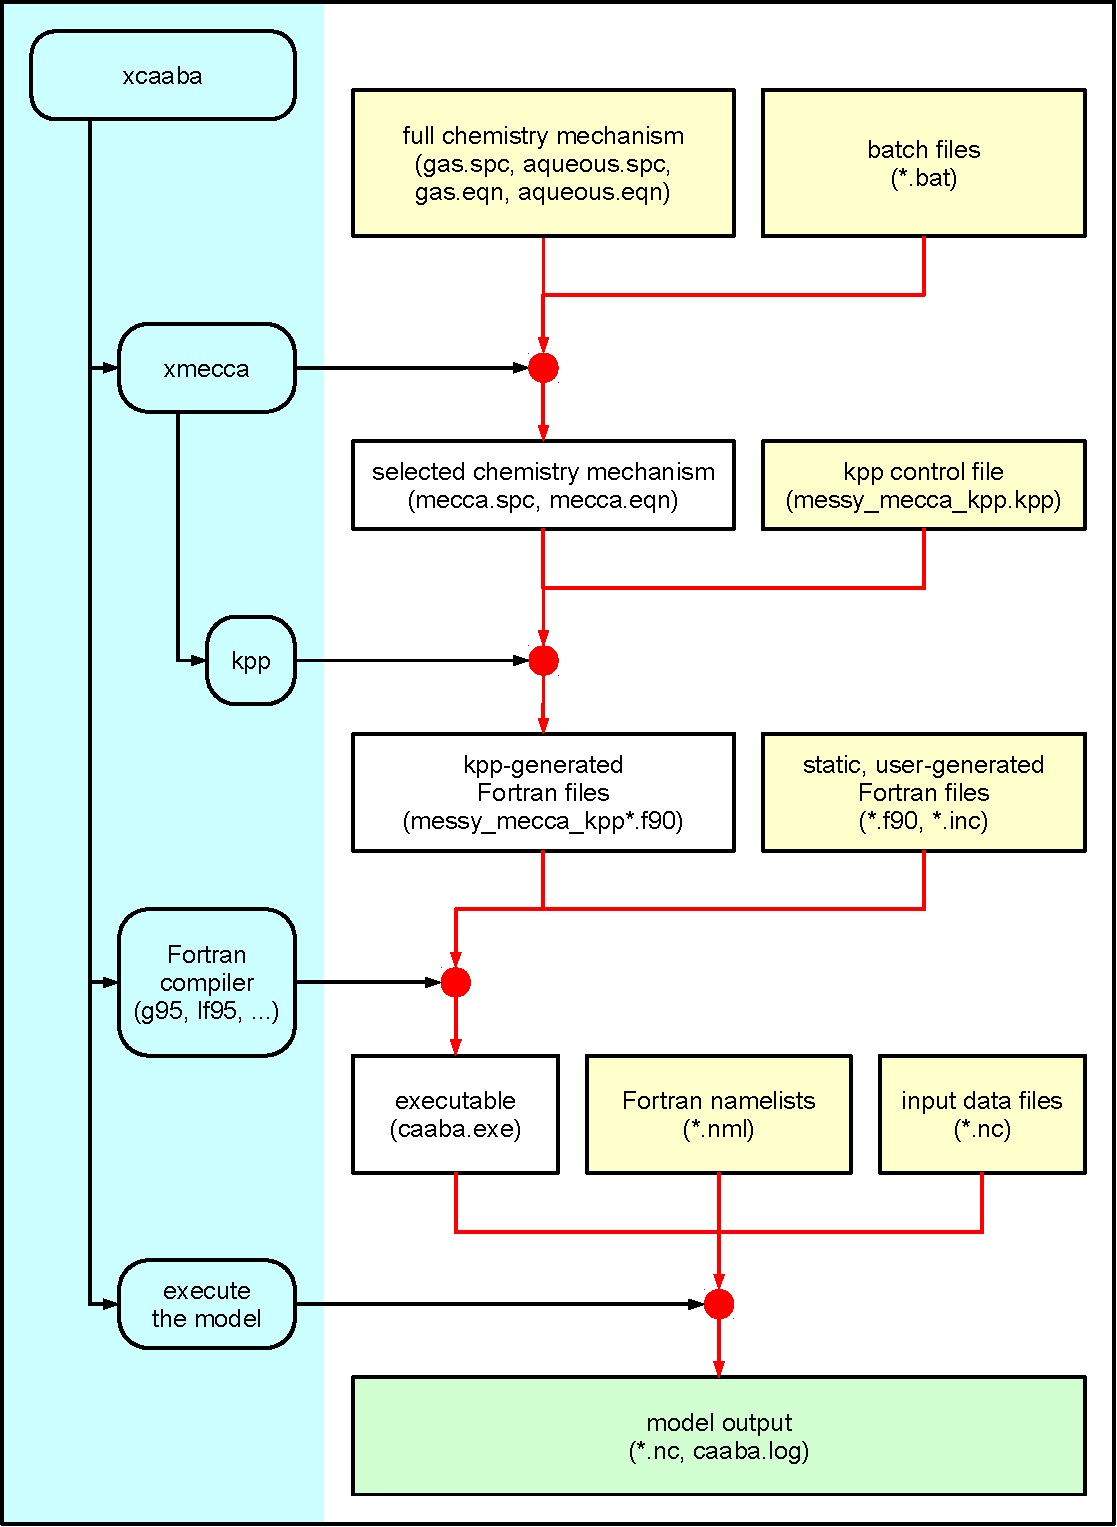
\includegraphics[width=0.9\textwidth]{flowcontrol_xcaaba}
  \end{center}
  \caption{Illustration of the tasks performed by \I{xcaaba}{\tt
      xcaaba.py}. {\tt xcaaba.py} and all scripts called by {\tt
      xcaaba.py} are shown on a blue background. User-generated (static)
    input files are shown on a yellow background whereas automatically
    generated temporary files are shown on a white background.}
  \label{fig:flowcontrol_xcaaba}
\end{figure*}

\begin{figure*}%[htb]
  \begin{center}
  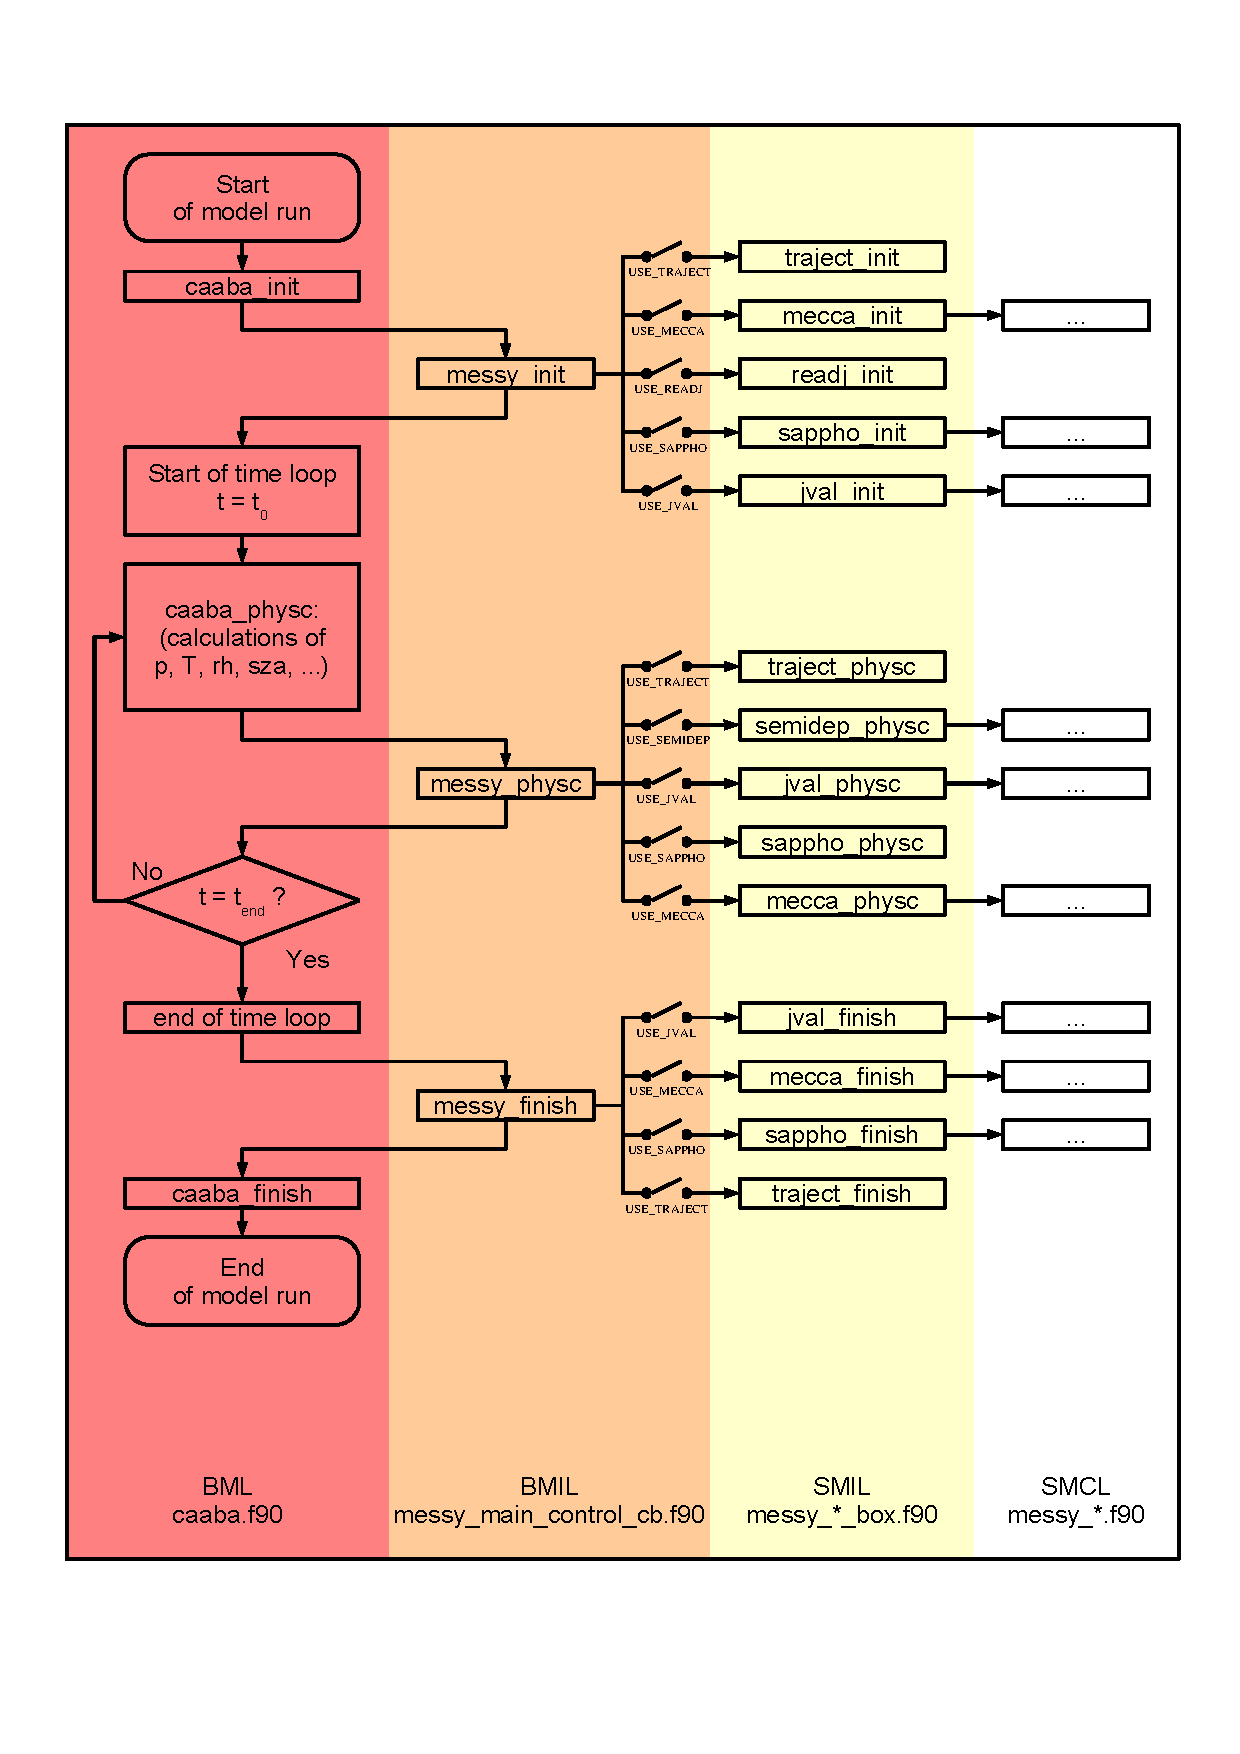
\includegraphics[width=\textwidth]{caaba_flowcontrol}
  \end{center}
  \caption{Flow control of a \IT{CAABA} \IT{box model} simulation}
  \label{fig:caaba_flowcontrol}
\end{figure*}

\section{Modular model structure}
\label{sec:submodels}

Several MESSy \IT{submodel}s are available for use with CAABA:

\subsection{\IT{MECCA}}
\label{sec:MECCA}

MECCA is the main submodel that calculates gas- and aqueous-phase
\IT{chemistry}. A detailed description is presented in this manual.

\subsection{Photolysis submodels}

\subsubsection{\IT{JVAL}}
\label{sec:JVAL}

\IT{JVAL} \citep{2342} is the standard photolysis submodel in CAABA. It
is used to calculate \IT{j-values}. A detailed description can be found
in Sect.~\ref{sec:jval}.

\subsubsection{\IT{DISSOC}}
\label{sec:DISSOC}

\IT{j-values} can be calculated with \IT{DISSOC}.

\subsubsection{\IT{RADJIMT}}
\label{sec:RADJIMT}

\IT{RADJIMT} provides dissociation and ionization rates due to
absorption of light and energetic photoelectrons in the mesosphere and
thermosphere.

\subsubsection{\IT{READJ}}
\label{sec:READJ}

\IT{READJ} reads $j$-values from lookup tables in netcdf files.

\subsubsection{\IT{SAPPHO}}
\label{sec:SAPPHO}

As a simple alternative, \IT{SAPPHO} calculates simplified and
parameterized \IT{photolysis} rates based on interpolation functions.

\subsection{Other}

\subsubsection{\IT{SEMIDEP}}
\label{sec:SEMIDEP}

\IT{SEMIDEP} calculates simplified \IT{emission} and \IT{deposition}.

\subsubsection{\IT{TRAJECT}}
\label{sec:TRAJECT}

The submodel \IT{TRAJECT} reads and processes input data to simulate an
air parcel along a prescribed trajectory (trajectory box model), as
described in Sect.~\ref{sec:lagrangian}. More generally, TRAJECT is used
to prescribe physical boundary conditions for the simulation as a
function of time, and thus can for instance also be used to simulate
laboratory conditions, such as temperature ramps during chemical
kinetics measurements.

\section{Miscellaneous \IT{CAABA/MECCA} features}
\label{sec:misc}

\subsection{\IT{Scenario}s}
\label{sec:scenarios}

To facilitate running \IT{CAABA} under different \IT{boundary
  conditions}, so-called ``\IT{scenario}s'' can be defined for
\IT{photolysis} (\I{photo\_scenario}\verb|photo_scenario|),
\IT{initialization} (\I{init\_scenario}\verb|init_scenario|),
\IT{photolysis} (\I{photo\_scenario}\verb|photo_scenario|),
\IT{emission} (\I{emission\_scenario}\verb|emission_scenario|), dry
\IT{deposition} (\I{drydep\_scenario}\verb|drydep_scenario|), and the
\I{aqueous phase}aqueous-phase composition
(\I{aqueous\_scenario}\verb|aqueous_scenario|). The variable
\I{list\_of\_scenarios}\verb|list_of_scenarios| in
\verb|caaba_module.f90| contains a complete list of \IT{scenario}s. Some
examples are:
\begin{center}
  \begin{tabular}{ll}
    \hrulefill & For testing: \quad\hrulefill\\
    \verb|ZEROAIR|       & very simple, clean air\\
    \verb|MOM|           & Mainz Organic Mechanism\\
    \hrulefill & Regions: \quad\hrulefill\\
    \verb|MBL|           & marine boundary layer\\
    \verb|FF_ANTARCTIC|  & Antarctic (frost flowers)\\
    \verb|FF_ARCTIC|     & Arctic (frost flowers)\\
    \hrulefill & Altitudes: \quad\hrulefill\\
    \verb|FREE_TROP|     & free troposphere\\
    \verb|TROPOPAUSE|    & tropopause ($\approx\ 220$ hPa)\\
    %\verb|STRATO|        & \\
    \verb|LOW_STRATO|    & stratosphere ($\approx\ 120$ hPa)\\
    \verb|MID_STRATO|    & stratosphere ($\approx\ 25$ hPa)\\
    \verb|HIGH_STRATO|   & stratosphere ($\approx\ 3$ hPa)\\
    \verb|MTCHEM|        & mesosphere ($\approx\ 0.01$ hPa)\\
    \hrulefill & Aqueous phase: \quad\hrulefill\\
    \verb|'LAB|          & laboratory (aerosol in cloud chamber)\\
    \verb|'VOLCANO|      & volcanic aerosol\\
    \verb|'CLOUD|        & cloud droplets\\
    %\hrulefill & Campaigns: \quad\hrulefill\\
    %\verb|CUMULUS|       & bright conditions inside a cloud top ($\approx\ 200$ hPa, tropics)\\
    %\verb|HOOVER|        & \\
    %\verb|OOMPH|         & \\
    \hrulefill & Other: \quad\hrulefill\\
    \verb|LAB|           & laboratory smog chamber\\
    %\verb|LAB_C15|       & \\
    %\verb|ISO|           & \\
    %\verb|TAG|           & \\
    \verb|VOLCANO|       & volcanic plume\\ 
  \end{tabular}
\end{center}

\begin{figure}%[htb]
  \begin{center}
    \fbox{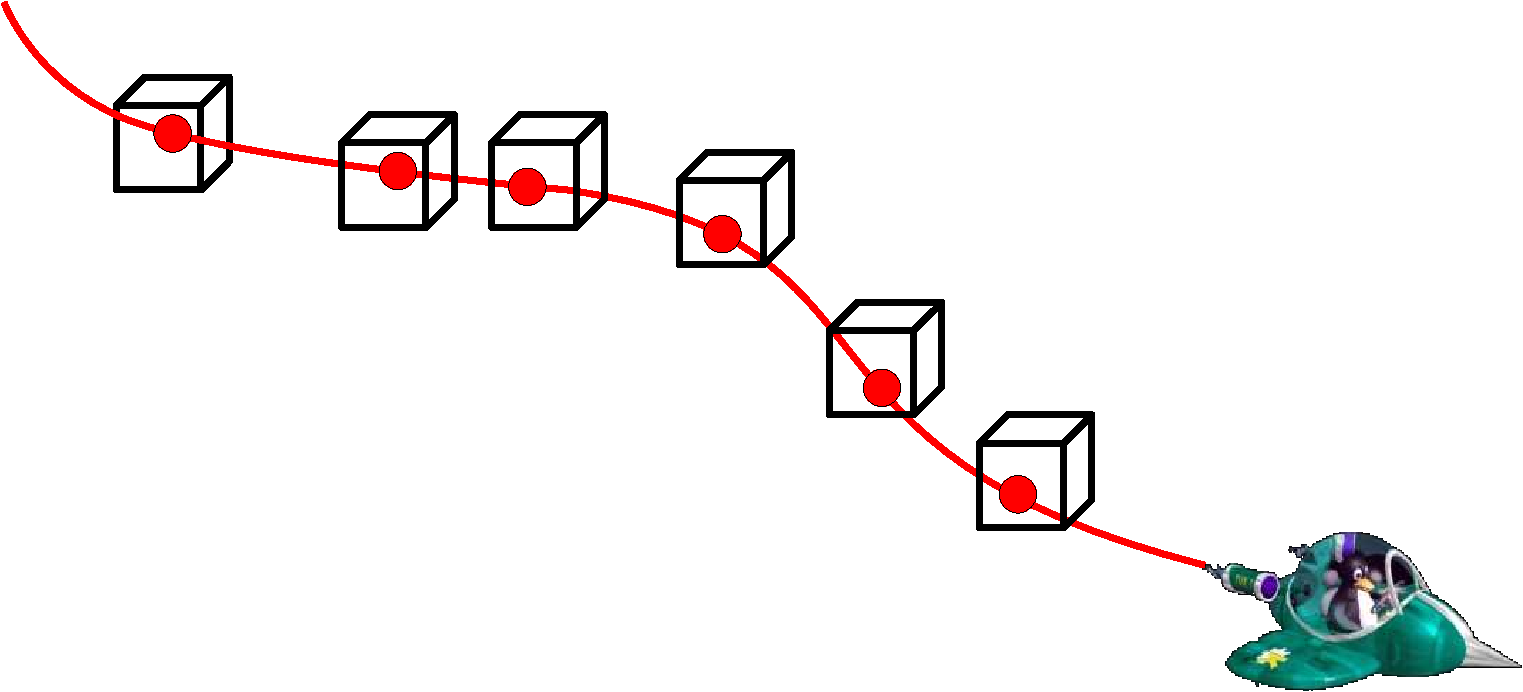
\includegraphics[width=0.95\columnwidth]{steady_state_model}}
  \end{center}
  \caption{Multiple model simulations performed to analyze measured data.}
  \label{fig:steady_state}
\end{figure}

\subsection{Multiple model simulations and \IT{steady state}
  (``multirun'')}
\label{sec:multirun}

The so-called ``multirun'' mode performs multiple model simulations.
Terminating them when a \IT{steady state} has been reached, this mode
can be useful to calculate the steady-state \IT{concentration}s of
short-lived species when the concentrations of longer-lived species
(e.g., non-methane \IT{hydrocarbon}s) are known from measurements, as
illustrated in Fig.~\ref{fig:steady_state}. The default termination
condition is that the relative change of \chem{OH} and \chem{HO_2}
between two model time steps is less than $10^{-6}$~\unit{s^{-1}}. If
necessary, this can be changed in the function
\verb|steady_state_reached| in \verb|messy_mecca.f90|. To avoid that the
concentrations of \IT{long-lived species} change from their initial
values, they should be fixed by setting \I{SETFIX}\verb|setfixlist| in
the batch file. An \IT{initialization} file for chemical species (see
Sect.~\ref{sec:tracfile}) and a \IT{photolysis} initialization file (see
Sect.~\ref{sec:readjfile}) must be available in the
\verb|input/multirun/| directory. As examples, the files
\verb|example_*.nc| are available. For first tests in the \IT{multirun
  mode}, it is recommended to use \verb|example_small.nc|. To create
input \IT{netCDF} files from \IT{ASCII} files, the script
\I{txt2nc.py}\verb|txt2nc.py| can be used (see below). After these
preparations, the \IT{multirun mode} can be entered by running
\I{xcaaba}\verb|xcaaba.py| and answering ``Run CAABA/MECCA?'' with
``\verb|m|''. The user can then select an input file from the
\verb|input/multirun/| directory. Next, the script
\I{multirun.py}\verb|multirun.py| is called. For each line in the input
file, \verb|multirun.py| first adjusts the \IT{namelist} file
\verb|caaba.nml| and then performs a \IT{CAABA/MECCA} model simulation.
After all model simulations have finished, a summary of the output is
placed in the output directory. The name of the output directory will be
based on the name of the input \IT{netCDF} file, e.g., when the file
\verb|example_small.nc| is used, the output will be in
\verb|output/multirun/example_small/|. The final \IT{concentration}s and
rate coefficients of all simulations are summarized in
\verb|caaba_mecca_c_end.nc| and \verb|caaba_mecca_k_end.nc|. Results of
the individual simulations can be found in the \verb|runs/|
subdirectory.

\subsubsection{Creating multirun input files with \I{txt2nc.py}{\tt
    txt2nc.py}}

If there are only \verb|*.txt| files in the input directory
\verb|input/multirun/| but no \verb|*.nc| files, then you have to create
them with the script \verb|txt2nc.py|, e.g.:
\begin{verbatim}
./txt2nc.py example_small.txt
\end{verbatim}
To create your own input \IT{netCDF} file, make a copy of
\verb|example_small.txt| (e.g., \verb|myfile.txt|) and edit that. The
following properties must be kept:
\begin{itemize}
\item The first line is a header that contains the variable names as
  they appear in the \IT{MECCA} \IT{chemistry} code.
\item The first column is the run number. The values can be anything as
  long as they increase from line to line. The name of this (or any
  other) column must not be ``\verb|time|''.
\item The columns ``\verb|press|'' and ``\verb|temp|'' are mandatory.
  \I{pressure}Pressure must be in [\I{Pascal>unit of pressure}Pa] and
  \IT{temperature} in [\I{Kelvin}K].
\item The file must be in \IT{UNIX} format with ``LF'', not in
  DOS format with ``CR/LF'' as the end-of-line
  character\footnote{\url{http://en.wikipedia.org/wiki/Newline}}. If
  necessary, \verb|txt2nc.py| tries to convert to the correct format.
\end{itemize}

\subsection{Monte-Carlo}
\label{sec:montecarlo}

\subsubsection{Performing Monte-Carlo simulations}

In the \IT{Monte-Carlo mode}, several \IT{CAABA/MECCA} simulations are
performed, with each individual simulation using slightly different rate
coefficients. To activate it, you first have to create a new chemical
\IT{reaction mechanism} with \I{xmecca}\verb|xmecca| (see
Sect.~\ref{sec:xmecca}) and answer the question ``Add Monte-Carlo factor
to all rate coefficients'' with ``\verb|y|'' (e.g., using the \IT{batch
  file} \verb|mcfct.bat|). This will start the \IT{gawk} script
\I{mcfct.awk}\verb|mcfct.awk|, which adds Monte-Carlo factors to the
rate coefficients in the equation file. Next, the
\I{xcaaba}\verb|xcaaba.py| script can be used interactively to start the
simulations with the \IT{namelist} \verb|caaba_mcfct.nml|.
Alternatively, the whole Monte-Carlo simulation can be performed in
batch mode using a config (\verb|*.ini|) file:
\begin{verbatim}
 ./xcaaba.py -i caaba_montecarlo.ini
\end{verbatim}
The script \I{montecarlo.py}\verb|montecarlo.py| in the directory
\verb|pycaaba/| will now perform the Monte-Carlo model simulations. The
default is to make 100 model simulations. To choose another value (up to
9999), change the definition of \verb|maxline| in \verb|montecarlo.py|.

\subsubsection{Plotting and analyzing Monte-Carlo simulations}

After performing the model simulations, the resulting \IT{netCDF} files
are merged and then stored in the output directory called
\verb|output/montecarlo/latest|. The final \IT{concentration}s and rate
coefficients of all simulations are summarized in
\verb|caaba_mecca_c_end.nc| and \verb|caaba_mecca_k_end.nc|. Results of
the individual simulations can be found in the \verb|runs/*|
subdirectories.

\paragraph{Time series}

The time series of all simulations can be plotted together with
\IT{caabaplot.py}. However, these plots become illegible if more than
about 5 simulations are made.

\paragraph{\I{steady state}Steady-state calculations}

The most efficient way to analyze a large number of Monte-Carlo
simulations is to use the steady-state option and only compare the final
values of the different model simulations, not the individual time
series. The script \verb|montecarloplot.py| can be used to create
scatter plots of \IT{concentration}s vs rate coefficients. For all
comparisons above a given threshold (\verb|MINR2 = 0.1|) of the
coefficient of determination ($r^2$), \IT{linear regression} lines are
plotted. Note, however, that $r^2$ is only an indicator of the goodness
of a {\em linear} correlation. It is also possible that the dependence
of a species on a rate coefficient is {\em nonlinear}.

\subsubsection{Variation of rate coefficients}

In each individual Monte-Carlo simulation $j$, all rate coefficients
$k_i$ are varied by a Monte-Carlo factor:

\begin{equation}
  k^{\rm MC}_{i,j} = k_i \times f_i^{x_{i,j}}
\end{equation}

Here, $k^{\rm MC}_{i,j}$ is the rate coefficient of reaction $i$ used in
the Monte-Carlo simulation $j$. It is defined as the product of the
recommended value $k_i$ and the Monte-Carlo factor $f_i^{x_{i,j}}$. This
Monte-Carlo factor consists of two parts, the uncertainty factor $f_i$
and the exponent $x_{i,j}$:

\paragraph{The uncertainty factor $f_i$}

The uncertainty factor $f_i$ describes the uncertainty of the measured
(or estimated) rate coefficient $k_i$. Its value can usually be found in
publications of laboratory studies or summaries like the \IT{JPL}
evaluation \citep{3245}.

The tables of the \IT{IUPAC} evaluations \egcite{1845} list the decadic
logarithm $\lg(f_i)$ of the uncertainty factor, which they call
``$\Delta\log k$''.

Sometimes an absolute uncertainty is quoted instead of an uncertainty
factor, e.g., $k = 2 \pm 0.2$ or $k = 2 \pm 10\%$. In this case we
define $f_i$ such that the upper limit is reached when multiplied with
$k_i$, i.e.\ in the current example $f_i = 1+0.2/2 = 1.1$.

The uncertainty factor is defined in the \IT{equation file}s
(\verb|*.eqn|) in a comment starting with the paragraph symbol. Three
different syntax types are possible:
\begin{itemize}
\item If there is just one \I{$\mathsection$ (in {\tt *.eqn}
    file)}\verb|§| sign, (e.g., ``\verb|{§1.1}|''), the value inside the
  \I{$\{\}$ (in {\tt *.eqn} file)}curly braces is the uncertainty factor
  $f_i$.
\item With two \verb|§| signs, (e.g., ``\verb|{§§0.04}|''), the value
  inside the curly braces equals $\lg(f_i)$.
\item If there is only a \verb|§| sign (``\verb|{§}|'') but no number,
  the uncertainty factor is set to the default value of $f_i$~= 1.25.
\end{itemize}

\paragraph{The Monte-Carlo exponent $x_{i,j}$}

\begin{figure}
  \begin{center}
    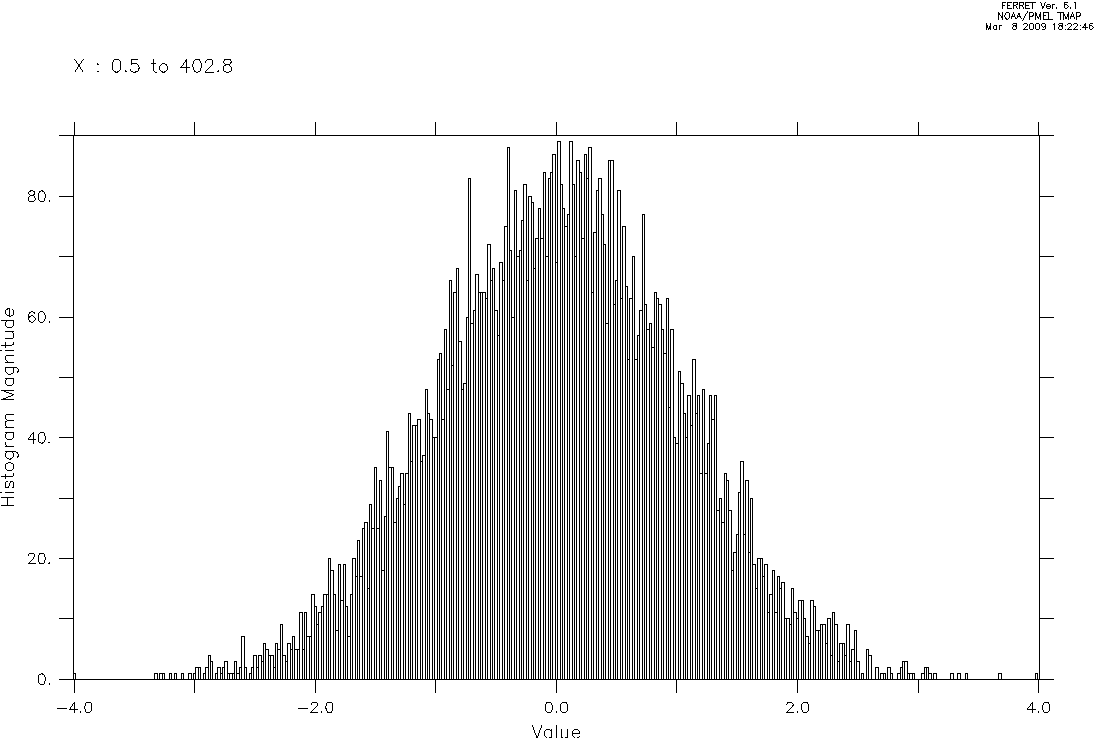
\includegraphics[width=\columnwidth]{random}
  \end{center}
  \caption{Example histogram of \I{normal
      distribution}normally-distributed \IT{random number}s.}
  \label{fig:random}
\end{figure}

There is one Monte-Carlo exponent $x_{i,j}$ (variable ``\verb|mcexp|''
in the code) for each rate coefficient $k_i$ and for each individual
Monte-Carlo simulation $j$. The values of $x_{i,j}$ are \I{normal
  distribution}normally-distributed \IT{random number}s centered around
zero (see Fig.~\ref{fig:random}), and produced with the \IT{Marsaglia
  polar method}
(\url{http://en.wikipedia.org/wiki/Marsaglia_polar_method}). As input
for the \IT{Marsaglia polar method}, uniformly distributed \IT{random
  number}s between 0 and 1 calculated with either the standard
\IT{Fortran95} function \verb|RANDOM_NUMBER| or the Mersenne Twister
algorithm \citep{2404} are used.

\subsubsection{Changing the uncertainty factors}

The uncertainty factors can be changed by modifying the equation files,
as shown in Sect.~\ref{sec:eqnfiles}. Note that predefined rate
coefficients (e.g., \verb|k_HO2_HO2|) already contain an uncertainty
factor and there must not be an additional factor in the reaction where
they are used.

In some cases, it may be useful to vary only one or a few rate
coefficients. To do this, it is first necessary to find the correct
indices of \verb|mcexp(...)| in \verb|mecca.eqn| (note that these
indices may change when creating a new \IT{reaction mechanism} with
\I{xmecca}\verb|xmecca|). As an example, to vary only the rate
coefficients that use \verb|mcexp(40)| and \verb|mcexp(50)|, the
following lines can be added to subroutine \verb|mecca_init| in
\verb|messy_mecca_box.f90| after \verb|CALL define_mcexp|:
\begin{verbatim}
DO i=1, MAX_MCEXP
  IF ((i/=40).OR.(i/=50)) mcexp(i) = 0.
ENDDO
\end{verbatim}

To verify that the rate coefficients are modified in the Monte-Carlo
simulations, it is possible to temporarily activate the subroutine
\verb|montecarlo_check| in \verb|template_messy_mecca_kpp.f90| and check
the output in \verb|caaba.log|. After these tests,
\verb|montecarlo_check| must be switched off again to allow normal model
simulations.

\subsection{\I{Lagrangian}TRAJECT: Prescribe physical conditions as
  function of time}
\label{sec:lagrangian}

\begin{figure}%[htb]
  \begin{center}
    \fbox{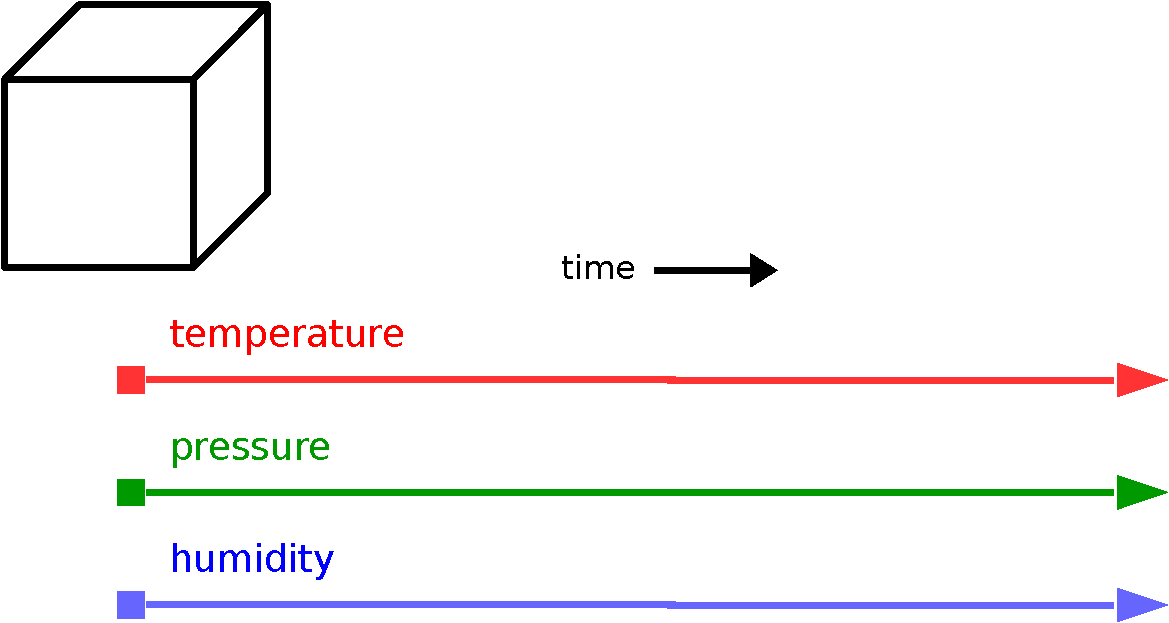
\includegraphics[width=0.95\columnwidth]{box_model_static}}\\[3mm]
    \fbox{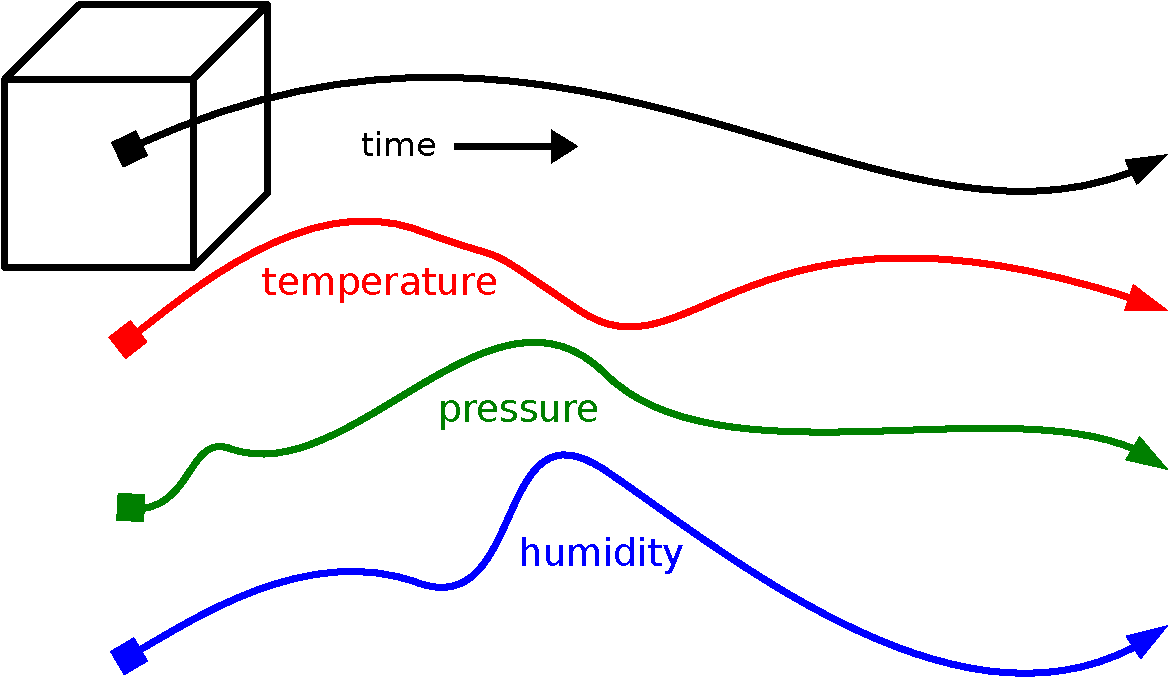
\includegraphics[width=0.95\columnwidth]{box_model_trajec}}
  \end{center}
  \caption{Top: As CAABA/MECCA focuses on chemistry, the meteorological
    parameters $T$, $p$ and RH are kept constant during the model
    simulation in the standard configuration. Bottom: For calculations
    along a trajectory, time-dependent values of $T$, $p$ and RH can be
    read from a file (see Sect.~\ref{sec:lagrangian} for details).}
  \label{fig:box_model}
\end{figure}

\begin{figure}%[htb]
  \begin{center}
    \fbox{\includegraphics[width=0.95\columnwidth]{traject_model}}
  \end{center}
  \caption{Multiple trajectory model simulations leading to the
    locations where measurements were made.}
  \label{fig:traject}
\end{figure}

\IT{CAABA} can be used as a \IT{Lagrangian} \IT{trajectory} \IT{box
  model} \citep{2403}, as illustrated in Fig.~\ref{fig:box_model}. For
example, multiple model simulations can be performed where each
trajectory leads to a measured data point (Fig.~\ref{fig:traject}). The
usual combination of \IT{submodel}s for this purpose includes the
\IT{CAABA} \IT{submodel} \IT{TRAJECT} for the processing of
\IT{trajectory} information, \IT{MECCA} for atmospheric \IT{chemistry},
and \IT{JVAL} for \IT{photolysis} rate calculation.

The TRAJECT submodel can be used for any application where physical
conditions change as a function of time, for instance experimental
setups in chemical kinetics laboratories, where physical parameters
are varied.

All important settings for \IT{trajectory} calculations can be made via the
\IT{namelist} file plus a few external files.

\subsubsection{\I{namelist}Namelist parameters}
\label{sec:trajnml}

A \IT{namelist} template can be found at \verb|nml/caaba_traject.nml|.
It is automatically available as namelist of choice when running
\IT{CAABA} via \I{xcaaba}\verb|xcaaba.py|. There are standard and
\IT{trajectory}-exclusive \IT{namelist} parameters to be set:
\begin{itemize}
\item \noindent\textbf{\I{submodel}Submodel switches (mandatory):} The
  \IT{trajectory} mode of \IT{CAABA} requires that
  \I{USE\_TRAJECT}\verb|USE_TRAJECT = T|,
  \I{USE\_MECCA}\verb|USE_MECCA = T|, and
  \I{USE\_JVAL}\verb|USE_JVAL = T| and/or
  \I{USE\_SAPPHO}\verb|USE_SAPPHO = T|. One of the two \IT{photolysis}
  rate models is sufficient, but it is also possible to run them in
  parallel (see also \verb|photrat_channel|). If the use of external
  \IT{photolysis} rate scaling based on $j$(\chem{NO_2}) is desired,
  \I{USE\_JVAL}\verb|USE_JVAL = T| is mandatory since the scaling of
  \IT{photolysis} rate coefficients is currently only implemented for
  \IT{JVAL}. For the application to atmospheric trajectories as in
  \citet{2403}, the \IT{submodel} \IT{SEMIDEP} was switched off.
\item \textbf{\I{scenario}Scenarios (optional):} The use of scenarios
  (see Sect.~\ref{sec:scenarios}) is
  optional in \IT{trajectory} mode. They can be used to supplement
  default values for unspecified \IT{photolysis} rate
  coefficients or initial \IT{mixing ratio}s. The values provided
  by external netCDF files override these values.
\item \textbf{\I{photolysis}Photolysis rate channel:} Since the scaling
  of \IT{photolysis} rate coefficients is currently only implemented for
  \IT{JVAL}, choose \I{photrat channel}\verb|photrat_channel = 'jval'|
  when planning to prescribe $j$(\chem{NO_2}) \IT{photolysis} rates.
\item \textbf{\I{trajectory}Trajectory input {\tt input\_physc}
    (mandatory):} The path to the \IT{netCDF} file containing physical
  information at \IT{trajectory} \IT{waypoint}s should be specified as,
  e.g., \code{input_physc = 'input/traject/example_input_physc.nc'}. For
  its structure, see section \ref{sec:trajfile}.
\item \textbf{\I{photolysis}Photolysis rates {\tt input\_jval}
    (optional):} To scale \IT{photolysis} rates with prescribed
  $j$(\chem{NO_2}) values, specify the path to the respective file as,
  e.g., \code{input_jval = 'input/traject/example_input_jval_no2.nc'}.
  For its structure, see \ref{sec:jvalfile}.
\item \textbf{Initialization of chemical species {\tt init\_spec}
    (optional):} \I{mixing ratio}Mixing ratios of chemical species can
  be initialized from an external \IT{netCDF} file by specifying the
  path to it, e.g., \I{init\_spec}\code{init_spec =
    'input/traject/example_init_spec.nc'}. For its structure, please
  refer to section \ref{sec:tracfile}. Without an external file,
  \IT{mixing ratio}s are initialized by \IT{box model} default or by the
  chosen \IT{scenario}. If both methods are used for a species, the
  value from the external \IT{netCDF} file will overwrite that from the
  subroutine \verb|x0_*| of the chosen \IT{scenario}. If only one time
  point is present in the file, then these mixing ratios are used to
  initialize the model, ignoring the time axis. If several points are
  present on the time axis, the time axis is used to interpolate mixing
  ratios to the exact model start time for initialization.
\item \textbf{All external input from one file (optional):}
  It is possible to provide all external input to \verb|TRAJECT| in
  one single file, see example file
  \code{input/traject/example_input_all.nc}.
\item \textbf{Variable names (optional):} There are default
  \IT{trajectory} variable names for \verb|input_physc| designated in
  \IT{CAABA}. They can be selectively changed by providing alternative
  variable names. Here is a list of \IT{trajectory} variables, their default
  name, and respective examples how to specify an alternative variable name:
  \begin{center}
    \begin{tabular}{lll}
      \hline
      quantity          & default        & alternatives\\
      \hline
      \IT{longitude}    & \verb|LON|     & \verb|vlon = 'TLON'|\\
      \IT{latitude}     & \verb|LAT|     & \verb|vlat = 'TLAT'|\\
      \IT{pressure}     & \verb|PRESS|   & \verb|vpress = 'TP'|\\
      \IT{temperature}  & \verb|TEMP|    & \verb|vtemp = 'TM1'|\\
      spec.\ humidity   & \verb|SPECHUM| & \verb|vspechum = 'sh'|\\
      rel.\  humidity   & (none)         & \verb|vrelhum = 'rh'|\\
      \IT{time}         & \verb|TIME|    & \verb|vtime = 'time'|\\
      \hline
    \end{tabular}
  \end{center}
  For only one of the two \IT{humidity} variables, an alternative name
  may be active in the \IT{namelist}. This is the variable that is
  subsequently used as humidity and that is internally converted to
  relative humidity or specific humidity if necessary. If none is given,
  then the specific humidity is used with the default name
  \verb|SPECHUM|. Both, specific humidity and relative humidity are
  written to output \verb|caaba_physc.nc|.
\item \textbf{Humidity options (optional):} To switch from the
  traditional simplified relative humidity definition to the \IT{WMO}
  definition, \verb|l_relhum_wmo = T| can be selected (see also
  Sect.~\ref{sec:trajfile}).

  By default, relative humidity is used to calculate the \IT{concentration}
  of water vapor $c$(\chem{H_2O}). If \verb|l_ignore_relhum = T|, then the
  relative humidity is ignored, and $c$(\chem{H_2O}) must be initialized
  in \verb|SUBROUTINE x0| (either directly or via external chemical
  \IT{initialization}).

  By default, the parameterizations from \citet{2553} for both, vapor
  \IT{pressure} over \IT{liquid} and over \IT{ice} are used. To use the
  \IT{saturation vapor pressure} parameterizations from
  \IT{ECHAM5/MESSy}, choose the \IT{namelist} entry
  \verb|l_hum_emac = T|.

  To always calculate saturation vapor pressure over liquid, disregarding
  temperature, set \verb|l_psat_liquid = T|.
\item \textbf{Time options (optional):}
  \verb|timesteplen_str| sets the integration and output \IT{time} step.
  See also Sect.~\ref{sec:caaba_nml}.

  Two \IT{namelist} parameters help to select only a part of a
  trajectory for simulation: \verb|runlast| defines the start point of
  the \IT{CAABA} simulation by counting backwards in time from the
  \IT{trajectory} end, i.e. \verb|runlast = 4.5| means ``calculate the
  last 4.5 days of the given \IT{trajectory}''. The \IT{unit} is days.
  The second parameter \verb|runtime_str| defines the overall model
  simulation \IT{time} (after applying \verb|runlast|). Thus,
  \verb|runlast| and \verb|runtime_str| combined select any desired part
  of the \IT{trajectory}.
\end{itemize}

\subsubsection{\I{trajectory}Trajectory input file {\tt input\_physc}}
\label{sec:trajfile}

The \IT{trajectory} information is provided to \IT{CAABA} via an
external \IT{netCDF} file, specified in the \IT{namelist} by
\verb|input_physc|. A sample file is available at
\code{input/traject/example_input_physc.nc}. The file must contain a
\IT{time} origin in 'seconds/minutes/hours/days since yyyy-mm-dd
hh:mm:ss', where the seconds in the \IT{time} string are optional, for
example: \verb|"MINUTES since 2000-01-19 08:00:00"|. The file must
contain at least two \IT{trajectory} \IT{waypoint}s and the following
\IT{time}-dependent variables:
\begin{center}
  \begin{tabular}{lll}
    \hline
    quantity            & default name   & \IT{unit}\\
    \hline
    \IT{longitude}      & \verb|LON|     & \IT{degree}s east\\
    \IT{latitude}       & \verb|LAT|     & \IT{degree}s north\\
    \IT{pressure}       & \verb|PRESS|   & \I{Pascal>unit of pressure}Pa\\
    \IT{temperature}    & \verb|TEMP|    & \I{Kelvin}K\\
    (specific humidity) & \verb|SPECHUM| & kg/kg\\
    (relative humidity) &                & 1\\
    \hline
  \end{tabular}
\end{center}

Even if one parameter is kept fixed (e.g., pressure), it must currently be
present in the file on the common trajectory time axis.

Of the two \IT{humidity} quantities, only one can be present. If
specific humidity is given, it is converted to relative humidity (RH)
within \IT{CAABA}. Depending on the \IT{namelist} parameter
\verb|l_relhum_wmo|, either the traditional definition of relative
humidity
\begin{equation}
 \mbox{RH} = \frac{p_{H_2O}(T)}{p_{\rm sat}(T)},
\end{equation}
or the \IT{WMO} definition \citep{3334}
\begin{equation}
\mbox{RH} = \frac{\omega_v}{\omega_{vs}} =
\frac{p_{\chem{H_2O}}(T)}{p - p_{\chem{H_2O}}(T)} \times
\frac{p - p_{\rm sat}(T)}{p_{\rm sat}(T)}
\end{equation}
is applied, with p = atmospheric \IT{pressure}, $p_{\chem{H_2O}}$
= water vapor partial pressure, $p_{\rm sat}$ = water
\IT{saturation vapor pressure}, $\omega_v$ = water vapor
\IT{mass mixing ratio}, and $\omega_{vs}$ = water saturation
vapor \IT{mass mixing ratio} in dry air. We calculate the latter
two as:
\begin{eqnarray}
  \omega_v & = & \frac{q}{1-q}\\
  \omega_{vs} & = & \frac{M(\chem{H_2O})}{M({\rm air})} \times
  \frac{p_{\rm sat}(T)}{p - p_{\rm sat}(T)},
\end{eqnarray}
using the \IT{temperature}-dependent water \IT{saturation vapor
  pressure} $p_{\rm sat}(T)$, and the \IT{molar mass}es $M$ of water and
dry air. There are two parameterization schemes available for the water
saturation vapor pressure, which can be selected by \IT{namelist} (see
Sect.~\ref{sec:trajnml}).

\begin{table*}%[htb]
  \begin{center}
    \caption{List of \IT{trajectory} mode output variables in {\tt
        caaba\_messy.nc}.}
    \label{tab:trajout}
    \begin{tabular}{lll}
      \hline
      variable         & \IT{unit}             & notes\\
      \hline
      \verb|time|      & {\em time unit} since {\em time origin} & \IT{UTC}\\
      \verb|lon|       & \IT{degree}s east        & \IT{longitude}\\
      \verb|lat|       & \IT{degree}s north       & \IT{latitude}\\
      \verb|press|     & \I{Pascal>unit of pressure}Pa & \IT{pressure}\\
      \verb|temp|      & \I{Kelvin}K      & \IT{temperature}\\
      \verb|relhum|    & 1                & relative \IT{humidity} (RH)\\
      \hline
      \verb|spechum|   & kg/kg            & specific humidity ($q$)\\
      \verb|sza|       & deg              & \IT{solar zenith angle}\\
      \verb|j_NO2_x|   & 1/s              & external \chem{NO_2} \IT{photolysis} rate for scaling\\
      \verb|localtime| & (same as time)   & local \IT{time} at \IT{trajectory} position\\
      \verb|year_loc|  &                  & year of local \IT{time}\\
      \verb|month_loc| &                  & month of local \IT{time}\\
      \verb|day_loc|   &                  & day of local \IT{time}\\
      \verb|hour_loc|  &                  & hour of local \IT{time}\\
      \verb|min_loc|   &                  & minute of local \IT{time}\\
      \verb|sec_loc|   &                  & second of local \IT{time}\\
      \hline
    \end{tabular}
  \end{center}
\end{table*}

\subsubsection{\I{photolysis}Photolysis rate input file {\tt
    input\_jval}}
\label{sec:jvalfile}

It is possible to scale \IT{photolysis} rate coefficients via prescribed
$j$(\chem{NO_2}) values from a \IT{netCDF} file. All photolysis rates are
then scaled as:
\begin{equation}
  j_X{\rm (scaled)} = j_X {\rm (JVAL)} \times
  \frac{J_{\rm NO_2} {\rm (external)}}{j_{\rm NO_2} {\rm (JVAL)}}
\end{equation}

An example input file is available at
\code{input/traject/example_input_jval_no2.nc}. The name in the
\IT{netCDF} file must be \verb|j_NO2|. The files specified in
\verb|input_jval| and \verb|input_physc| must refer to exactly the same
\IT{trajectory} with the same time axis, because the $j$-values are read
into the model at the same times as other \IT{trajectory} information
and not further interpolated. As mentioned above, it is possible to have
only one file that contains all necessary information and insert that
file name for both, \verb|input_jval| and \verb|input_physc|. If no
\verb|input_jval| file is given then no scaling is applied to the
photolysis rates.

\subsubsection{\I{trajectory}TRAJECT mode output}
\label{sec:trajout}

In TRAJECT mode, all trajectory waypoints from the input files will be
present in the output files. If necessary, additional output time steps
are inserted to ensure this. If trajectory waypoints do not coincide
with the model time stepping (default or specified in the namelist),
then the output files will thus contain more points than the input files
(trajectory waypoints + regular time stepping points).

Physical output along the \IT{trajectory} is written to \verb|caaba_messy.nc|.
There are some special variables written out in addition to the default
\verb|caaba_messy.nc| output. These are listed in the second part of
Tab.~\ref{tab:trajout}, below the middle line.

Mixing ratios as simulated by \verb|MECCA| are written to the usual
output file \verb|caaba_mecca.nc|, and $j$-values to
\verb|caaba_jval.nc|. Unlike the default CAABA output, TRAJECT mode
output is one-dimensional, without any 3D dummy variables, to free up
the standard names LON and LAT for the trajectory variables. The output
now always contains specific humidity as well as relative humidity.

\subsection{\I{tagging}Tagging diagnostics and \IT{isotope}
  modeling}
\label{sec:tag}

Before using the tagging feature, please make sure that version 2.6.0 or
higher of \I{fpc}\verb|fpc| (Free \I{Pascal>programming language}Pascal
\IT{compiler}, \url{http://www.freepascal.org/}) is installed and
configured on your system. To create an (isotopically) tagged
\IT{reaction mechanism} with \I{xmecca}\verb|xmecca|, the \IT{batch
  file} options \verb|tag| and \verb|tagcfg| can be used. Before running
\IT{CAABA/MECCA}, the execution of the tagging code has to be enabled by
setting \verb|l_tag=T| in the \I{CTRL}\verb|&CTRL| \IT{namelist} in
\verb|mecca.nml|. When tagging is used, the model simulation may produce
additional files \verb|caaba_mecca_tag_*.nc| containing output from the
tagged part of the mechanism, e.g., fractions of tagged counterparts or
isotope ratios of isotopologues. The batch file \verb|iso_example.bat|
contains a simple example of the \chem{^{12}C}/\chem{^{13}C} isotopes of
methane tagging. Further tagging configurations can be found by running
\verb|xmecca| interactively (without using a batch file) and answering
``\verb|y|'' to the question about tagging. To obtain further details,
read \citet{2504} and contact Sergey Gromov
\url{<sergey.gromov@mpic.de>}.

\subsection{\I{skeleton}Skeletal \I{mechanism reduction}mechanism generation}
\label{sec:skeleton}

Creating a skeletal mechanism involves several steps: First, the sample
points must be defined, i.e., the conditions under which the skeletal
mechanisms are compared to the full mechanism. Next, the setup must be
defined, in particular the full mechanism (\verb|skeleton.bat|), the
target species (\verb|targets.txt|), the namelist file (via
\verb|multirun.py|), and a control file (\verb|ctrl/*.py|). Finally, the
skeletal mechanism generation can be started with \verb|xskeleton.py|.
To analyze the results, several plots and data files are generated
automatically.

\subsubsection{Creating sample points}

\paragraph{Extracting sample points from CAABA/MECCA box model results}

First, perform several box model simulations under conditions that
represent the desired sample points. In the batch file, choose the full
chemistry mechanism and switch off the output of reaction rates
(\verb|set rxnrates = n|).

To obtain typical daytime concentrations, ensure that the model
simulation ends during the day (\verb|model_start_day| and
\verb|runtime_str| in the namelist file), e.g., at noon. The resulting
output files must be merged with:\\
\verb|ncks -A caaba_messy.nc all.nc|\\
\verb|ncks -A caaba_mecca.nc all.nc|\\
\verb|ncks -A caaba_jval.nc  all.nc|\\
Then, the last timestep can be extracted with:\\
\verb|ncks -F -O -d time,-1 all.nc t_final.nc|\\
After performing several model simulations under various conditions,
merge the resulting netCDF files (\verb|*/t_final.nc|) from all sample
points:\\
\verb|ncrcat -O */t_final.nc skeleton_samplepoints.nc|\\
Finally, consecutively numbered values (1,2,3,\dots) must be entered
into the time dimension of the resulting file
\verb|skeleton_samplepoints.nc|. This can be done via ncdump and ncgen.

\paragraph{Extracting sample points from global model results with the
  \IT{python} script \I{extract\_sample points.py}{\tt
    extract\_samplepoints.py}}

The script \verb|extract_samplepoints.py| in the \verb|samplepoints/|
directory extracts several grid boxes from the output of a global
ECHAM5/MESSy model simulation. These cover a broad range of
environmental conditions and will be used as initial conditions for the
box model simulations. When extracting sample points for specific
conditions (e.g., low concentrations of organic species) set
\begin{verbatim}
MASK = 'loworg'
\end{verbatim}
and define the \verb|mask| variable accordingly. The script must be run
on a computer which has access to the global model results, e.g.,
\verb|mistral.dkrz.de|. Data from the selected grid boxes are written to
a netcdf file in the \verb|samplepoints/| directory, e.g.,
\verb|skeleton_samplepoints_30_loworg.nc|. A file with the same base
name but a suffix \verb|pdf| instead of \verb|nc| shows plots
summarizing the chemical composition of all sample points.

\subsubsection{Setup}

Edit \verb|skeleton.bat| to define the full mechanism. Use
\verb|gaseqnfile| and \verb|wanted| but do not change \verb|rplfile|
because ``\verb|set rplfile = skeleton|'' is needed by
\verb|xskeleton.py|.

Ensure that the namelist file generated by
\I{multirun.py}\verb|multirun.py| is suitable.

Define the target species and their acceptable error tolerances in
\verb|targets.txt|.

Choose and/or edit a control file, e.g., \verb|ctrl/lowterp.py|. It must
contain the name of a sample point file, e.g.:
\begin{verbatim}
samplepointfilename='skeleton_samplepoints_30'
\end{verbatim}
Also, the variables \verb|eps|, \verb|eps_increase|, and some plotting
options can be defined in the control file.

\subsubsection{Creating a skeletal mechanism with the \IT{python} script
  \I{xskeleton.py}{\tt xskeleton.py}}

Run the \IT{python} script \verb|xskeleton.py| and supply the basename
of the control file as a parameter, e.g.:
\begin{verbatim}
xskeleton.py lowterp
\end{verbatim}
This will perform the following actions:

\begin{enumerate}
\item Run the model with the full mechanism (from \verb|skeleton.bat|).
\item The Fortran95 code \verb|oic.f90| calculates the overall
  interaction coefficients (OICs) of the \verb|NVAR| variable (not
  fixed) species for the full mechanism.
\item Loop over trial skeletal mechanisms:
  \begin{enumerate}
  \item Run the CAABA/MECCA model with the current skeletal mechanism.
  \item Calculate the error relative to the full mechanism.
  \item Exit the loop when the error has become too big.
  \end{enumerate}
\item A \verb|skeleton/| subdirectory is created inside the
  \verb|caaba/output/| directory. Plots (\verb|*.pdf|) and data files
  (\verb|*.dat|) describing the skeletal mechanisms and model results
  are written into this directory.
\end{enumerate}

\subsubsection{Analyzing the skeletal mechanisms}

Several plots and data files are generated by \verb|xskeleton.py| which
can be used to analyze the skeletal mechanisms:

\begin{itemize}
\item \verb|xskeleton.log|: A log file containing the screen output of
  \verb|xskeleton.py|.
\item \verb|species.dat|: A list of species with their OIC values and
  the information in which of the skeletal mechanisms they are included.
\item \verb|reactions.dat|: A list of reactions and the information in
  which of the skeletal mechanisms they are included.
\item \verb|rates.dat|: A list of rates and how they have changed since
  the previous skeletal mechanism.
\item \verb|skeleton.rpl|: The best replacement file.
\item \verb|skeleton_*/skel_error.dat|: Errors of skeletal mechanisms
  for all sample points and targets.
\item \verb|delta_skel.pdf|: Plots showing (for all sample points and
  targets) how the error increases when the skeletal mechanisms get
  smaller.
\item \verb|targets.pdf|: Plots showing the time series of the target
  species (for all sample points and skeletal mechanisms).
\item \verb|samplepoint_|{\em nnnn}\verb|.pdf|: Plots showing the time
  series of all species (for all skeletal mechanisms) for sample point
  number {\em nnnn}.
\end{itemize}

\subsection{Other chemistry mechanisms}
\label{sec:othereqn}

Normally, MECCA uses the chemistry mechanism that is defined in the
\verb|gas.eqn| file. However, several other mechanisms are provided as
well. These are contained in the \verb|eqn/| subdirectory.

\subsubsection{CB05BASCOE}
\label{sec:cb05bascoe}

To activate the CB05BASCOE chemistry from the ECMWF Integrated
Forecasting System (IFS), run \verb|xmecca| with the
\verb|cb05bascoe.bat| batch file which uses the KPP equation file
\verb|cb05bascoe.eqn|.

\subsubsection{MOZART}
\label{sec:mozart}

To activate the MOZART chemistry from the ECMWF Integrated Forecasting
System (IFS), run \verb|xmecca| with the \verb|mozart.bat| batch file
which uses the KPP equation file \verb|mozart.eqn|.

\subsubsection{JAM}
\label{sec:jam}

To activate the J\"ulich Atmospheric Mechanism (JAM002), run
\verb|xmecca| with the \verb|jam.bat| batch file which uses the KPP
equation file \verb|jam002b_20170510mgs.eqn|.

\subsubsection{MCM}
\label{sec:mcm}

The tool \verb|xmcm2mecca| in the \verb|mecca/eqn/mcm/| subdirectory
allows to import reactions from the Master Chemical Mechanism (MCM). To
extract all reactions related to a specific species (as an example we
use limonene), mark it on the MCM web page
(\url{http://mcm.leeds.ac.uk/MCM}), then click on the ``Extract'' link.
Select ``KPP, experimental KPP format'' as the format in which you would
like to generate the sub-mechanism and activate the checkbox ``Include
generic rate coefficients?''. Click the ``Extract'' button and save the
file into the \verb|mecca/eqn/mcm/| directory. Instead of the default
name \verb|MCM_subset.kpp|, it is recommended to use a more meaningful
filename, e.g., \verb|limonene.kpp|. Now execute the shell script
\verb|xmcm2mecca| and provide the filename (with or without the suffix
\verb|.kpp|) as an argument:

\verb|cd mecca/eqn/mcm/|\\
\verb|./xmcm2mecca limonene|

The script generates two files, one describing the species
(\verb|limonene.spc|) and the other containing the imported equations
(\verb|limonene.eqn|). Detailed information about the conversion process
can be found in the log file \verb|xmcm2mecca.log|. In order to use the
mechanism in MECCA, specify the species and equation files in a batch
file, e.g., \verb|limonene.bat|:

\verb|set gasspcfile = eqn/mcm/limonene.spc|
\verb|set gaseqnfile = eqn/mcm/limonene.eqn|

Then run \verb|xmecca|, e.g.:

\verb|./xmecca limonene|

If an error occurs, the logfile \verb|xmcm2mecca.log| should be
consulted. For example, it lists the corresponding line if an
unidentifiable source of H2O was found in the input file. For some
reactions, H2O must be added to the products, e.g., if

\verb|OH + HCHO = HO2 + CO|

was found in equation file, it must be changed to:

\verb|OH + HCHO = H2O + HO2 + CO|

If MECCA finds two equations with identical reactants and products,
either one equation has to be deleted or a \verb|Dummy| product has to
be added to one of the equations, e.g.:

\verb|CClCONO3 + hv = HO2 + CO + CHOCl + NO2|
\verb|CClCONO3 + hv = Dummy + CHOCl + CO + HO2 + NO2|

\begin{figure*}
  \begin{center}
    \fbox{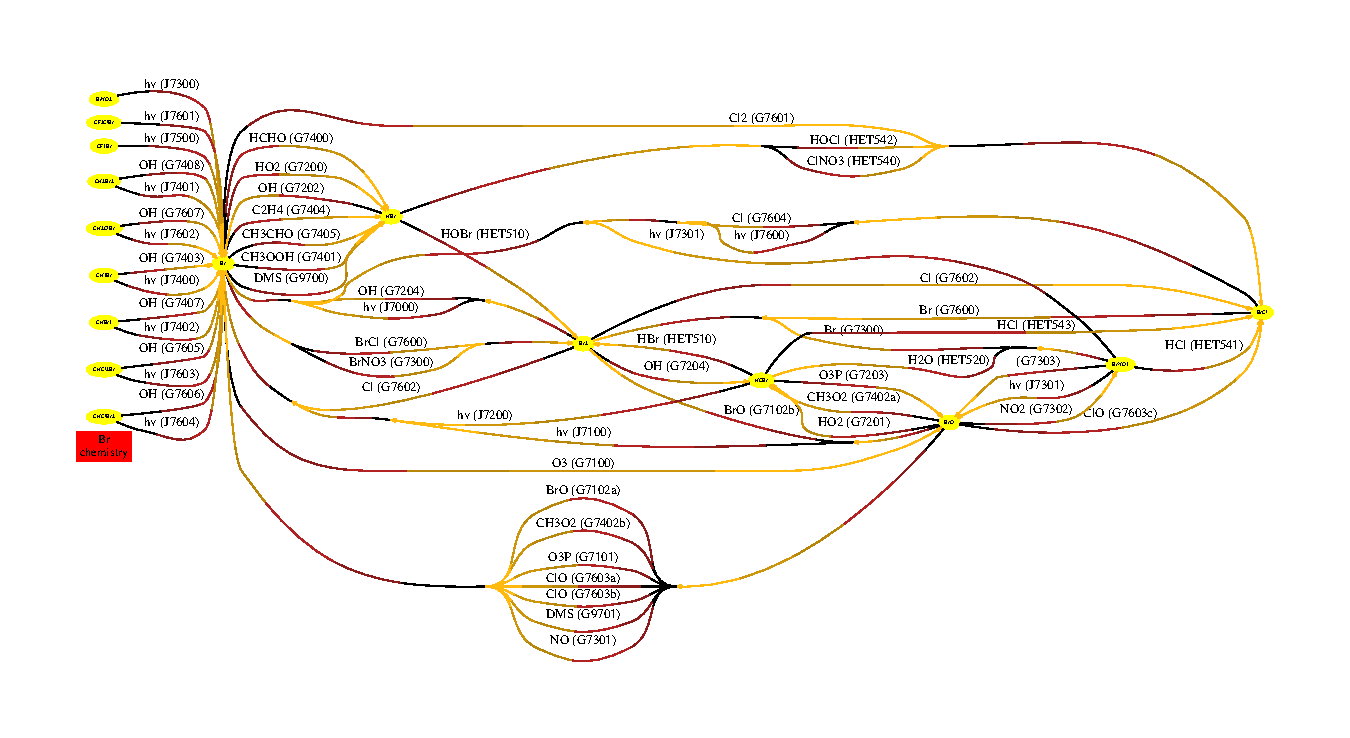
\includegraphics[width=0.9\textwidth]{mecca_Br}}
  \end{center}
  \caption{Visualization of the \IT{MECCA} \I{gas
      phase}gas-phase \IT{bromine} \IT{chemistry}
    generated with the \IT{graphviz} software.}
  \label{fig:Br}
\end{figure*}

\section{Visualization}
\label{sec:visualization}

If you have chosen \IT{netCDF} output, you can plot the model results
with either matplotlib of ferret. To visualize the chemical mechanism as
a graph, either the graphviz or the graph-tool software can be used.

\subsection{Plotting model results with the \IT{python} \IT{matplotlib}
  software}
\label{sec:matplotlib}

Start the \IT{python} script \verb|caabaplot.py|:
\begin{verbatim}
./caabaplot.py
\end{verbatim}

This will create the file \verb|xxxg.pdf| in the \verb|output/|
directory, containing plots of several species.

If the model simulation also created output files with reaction rates,
these will be shown in the file \verb|rxnrates.pdf|. To plot sources and
sinks, selected species can be entered in the subroutine
\verb|makeplots_rxnrates_scaled| which will create the file
\verb|rxnrates_scaled.pdf|.

The $j$-values of photolysis reactions are plotted in the file
\verb|jval.pdf|.

To plot results from previous simulations which are saved in the
\verb|output/| directory, create a config file and define
``\verb|modelruns|'' in the \verb|[caabaplot]| section. To compare model
simulations, you can enter several modelruns.

More information about matplotlib is available at
\url{https://matplotlib.org}.

\subsection{Plotting model results with the \IT{ferret} software}
\label{sec:ferret}

Note: It is recommended now to use matplotlib for plotting CAABA/MECCA
model results. Ferret is not supported anymore, and the description here
may be outdated.

Change into the \verb|jnl/| directory:
\begin{verbatim}
cd jnl
\end{verbatim}
Then start the ferret program:
\begin{verbatim}
ferret
\end{verbatim}
After ferret has started, you can type ferret commands at the command
line prompt ``yes?'' (to quit ferret, type ``q''). You can plot the
\I{gas phase}gas-phase species of the latest model simulation with the
ferret script \verb|xxxg.jnl| by typing:
\begin{verbatim}
go xxxg.jnl
\end{verbatim}
Similarly, \verb|xxxa.jnl| can be used to plot \I{aqueous
  phase}aqueous-phase species:
\begin{verbatim}
go xxxa.jnl
\end{verbatim}
The file \verb|xxxa.jnl| accepts several parameters to modify the plots.
The first parameter should be ``\verb|0d|'' for plotting \IT{box model}
results. The second parameter can be set to ``\verb|mpl|'' or
``\verb|mpm|'' in order to plot either \I{aqueous phase}aqueous-phase
\IT{concentration}s in \underline{m}ole \underline{p}er
\underline{l}iter or \IT{mixing ratio}s in \underline{m}ole
\underline{p}er \underline{m}ole, respectively. The third parameter
defines the \IT{aerosol} bin. With two \IT{aerosol} bins, ``\verb|A01|''
refers to sulfate \IT{particle}s, and ``\verb|A02|'' to sea-salt
\IT{particle}s. For example, type:
\begin{verbatim}
go xxxa.jnl 0d mpl A02
\end{verbatim}
\I{photolysis}Photolysis rate coefficients can be plotted with
\verb|jval.jnl|:
\begin{verbatim}
go jval.jnl
\end{verbatim}
If the calculation of accumulated \IT{reaction rate}s had been switched
on in \I{xmecca}\verb|xmecca| (see Sect.~~\ref{sec:xmecca}), plots of
the \IT{reaction rate}s can be made. One possibility is to plot all
reactions with:
\begin{verbatim}
go rxnrates.jnl
\end{verbatim}
Alternatively, it is possible to plot only the production and
destruction rates for a certain species, e.g., for OH:
\begin{verbatim}
go rxnrates_scaled.jnl OH
\end{verbatim}
To plot results from previous simulations which are saved in the
\verb|output/| directory, edit the file
\I{setmodelrun.jnl}\verb|setmodelrun.jnl| and enter the paths of the
directories in the ``\verb|GO _define_sensi|'' command. To compare model
simulations, you can enter two or more ``\verb|GO _define_sensi|''
commands in \verb|setmodelrun.jnl|. To plot the difference between model
simulations, activate the line ``\verb|DEFINE SYMBOL diffplot TRUE|'' in
\verb|setmodelrun.jnl|.

\subsection{Plotting the mechanism with \IT{graphviz}}
\label{sec:graphviz}

The files \verb|xgraphvizall|, \verb|xgraphviz|, and
\verb|spc_extract.awk| in the \verb|mecca/graphviz/| directory use the
graphviz software to visualize a chemical mechanism. Normally, these
scripts are started via \verb|xmecca|. As an example, the
graphviz-generated plot of \I{gas phase}gas-phase \IT{bromine}
\IT{chemistry} is shown in Fig.~\ref{fig:Br}.

\subsection{Plotting the mechanism with \IT{graph-tool}}
\label{sec:graph-tool}

Several \IT{python} subroutines are available in the
\verb|mecca/graphtool/| directory to visualize and analyse chemical
mechanisms with the graph-tool software \citep{3367}.

The script \verb|define_graph.py| uses input from \verb|mecca.spc|,
\verb|mecca.eqn|, and \verb|messy_mecca_kpp_parameters.f90| to define a
graph and save it in the file \verb|mecca_graph.xml.gz|. The vertices of
the graph represent the chemical species of the mechanism, i.e., all
species XYZ for which \verb|ind_XYZ| in
\verb|messy_mecca_kpp_parameters.f90| is non-zero. The elemental
composition of the species is taken from \verb|mecca.spc|. The edges of
the graph represent the chemical reactions in \verb|mecca.eqn|,
including equation tags (Sect.~\ref{sec:eqntags}) and the stoichiometry.

The script \verb|show_graph.py| reads the graph from
\verb|mecca_graph.xml.gz|. In addition, reaction rates from
\verb|caaba_mecca_rr.nc| and OIC values (Sect.~\ref{sec:skeleton}) from
\verb|OIC.dat| can be used as input. There are several possibilities to
analyze and visualize the mechanism:

\begin{itemize}
\item Filter the graph to show only a subset of the mechanism, e.g.,
  only organics containing a specified number of C atoms.
\item Calculate the maximum flow (Edmonds-Karp, push-relabel or
  Boykov-Kolmogorov algorithm) from a source to a target species, using
  reaction rates from \verb|caaba_mecca_rr.nc|.
\item Compare different skeletal mechanisms by color-coding species
  based on OIC values from \verb|OIC.dat|.
\item Analyze miscellaneous graph properties, e.g., Katz centrality.
\item Create an interactive GTK+ window
  (\url{https://graph-tool.skewed.de/static/doc/draw.html#graph_tool.draw.interactive_window}).
\end{itemize}

\section{Modifying \IT{CAABA/MECCA}}
\label{sec:modifying}

The \IT{CAABA/MECCA} model simulation can be modified by changing the
input files (\verb|*.nc|), the \IT{namelist} files (\verb|*.nml|), the
\IT{species file}s (\verb|*.spc|), the \IT{equation file}s
(\verb|*.eqn|) and the \IT{Fortran95} files (\verb|*.f90|). Frequently
applied changes are:
\begin{itemize}
\item Change the model \IT{time} (start, stop),
  \IT{location} (lon, lat), and/or \IT{meteorology} ($p$,
  $T$, RH) $\TO$ Sect.~\ref{sec:caaba_nml}
\item Add, delete, and change individual chemical reactions $\TO$
  Sect.~\ref{sec:expandchem}
\item Create or change the set of initial \IT{mixing ratio}s
  $\TO$ Sect.~\ref{sec:newscenario}
\item Create or change the set of \IT{photolysis} rate
  coefficients $\TO$ Sect.~\ref{sec:newscenario}
\item Create or change the set of \IT{emission} fluxes $\TO$
  Sect.~\ref{sec:newscenario}
\item Create or change the set of \IT{deposition} velocities
  $\TO$ Sect.~\ref{sec:newscenario}
\item Create or change the aqueous-phase composition
  $\TO$ Sect.~\ref{sec:newscenario}
\item Change the model \IT{initialization} using input files
  $\TO$ Sect.~\ref{sec:inputfiles}
\end{itemize}
The following sections describe typical (mostly minor) changes to the
model that are probably needed by many users. If you would like to make
extensive changes/additions to the model, please follow also the general
programming guidelines described in Sect.~\ref{sec:guidelines}.

\subsection{\I{namelist}Namelist files}
\label{sec:nmlfiles}

\IT{Fortran95} \IT{namelist} files allow modifications of the model
simulation without having to recompile the source code. The following
sections explain how to control a model simulation using
\code{caaba.nml} and other namelist files. Section~\ref{sec:nml_addvar}
explains how to add new variables to these namelists.

\subsubsection{The \IT{CAABA} \IT{namelist} file {\tt
    caaba.nml}}
\label{sec:caaba_nml}

The \verb|nml/| directory contains several \IT{namelist} files
\verb|nml/caaba_*.nml| with different settings for the \IT{namelist}
\verb|&CAABA|. Most of them can be edited directly to change the
settings of the model simulations. Only when the \IT{multirun mode} is
used, it is necessary to make the changes in the file
\I{multirun.py}\verb|multirun.py| in the \verb|pycaaba/| directory. The
link \verb|caaba.nml| points to the currently active \IT{namelist}.

Individual parts of the \IT{CAABA} model (the ``\IT{MESSy}
\IT{submodel}s'') can be switched on or off in \verb|caaba.nml|. For a
standard model simulation, it is important that the following switches
are set to ``\verb|T|'' (=true):
\I{USE\_MECCA}\I{USE\_JVAL}\I{USE\_SEMIDEP}
\begin{verbatim}
USE_MECCA   = T
USE_JVAL    = T
USE_SEMIDEP = T
\end{verbatim}
To use the \IT{photolysis} rate coefficients from \IT{JVAL} in
\IT{MECCA}, set:
\begin{verbatim}
photrat_channel = 'jval'
\end{verbatim}
Alternatively, you can switch on the \IT{SAPPHO} (or \IT{DISSOC})
\IT{submodel} with \I{USE\_SAPPHO}\verb|USE_SAPPHO = T| and then select
\I{photrat channel}\verb|photrat_channel = 'sappho'|. It is fine to
switch on more than one photolysis \IT{submodel}, this can be useful for
a comparison. However, only the values selected by
\verb|photrat_channel| are used for the \IT{MECCA} \IT{chemistry}.

You can define the model start, runtime, and \IT{time} step, e.g.:
\begin{verbatim}
model_start_day = 90.
runtime_str     = '10 days'
timesteplen_str = '15 minutes'
\end{verbatim}
If you don't set these, the default is a model start on day-of-year
(``Julian Day'') 80, a model simulation duration of 8 days, and an
output \IT{time} step of 20 minutes. The \verb|timesteplen_str| value
can be given as any \IT{integer} or \IT{floating point} in the
\IT{unit}s of \verb|seconds|, \verb|minutes|, or \verb|hours|.

The default is to output and sync every time step. For very long model
simulations, it can be useful to change these output and synchronization
frequencies, e.g.:
\begin{verbatim}
output_step_freq = 3
output_sync_freq = 1000
\end{verbatim}

As an alternative to a prescribed duration of the model simulation, it
is possible to stop the model simulation when a \IT{steady state} has
been reached. This is normally used in the ``multirun'' mode
(Sect.~\ref{sec:multirun}):
\begin{verbatim}
l_steady_state_stop = T
\end{verbatim}
The default \IT{location} of the model simulation (\IT{latitude},
\IT{longitude}) is 45$^\circ$ N and 0$^\circ$ E. It can be changed with
e.g.:
\begin{verbatim}
degree_lat = 82.  ! Alert
degree_lon = 297. ! Canada
\end{verbatim}
Changing the \IT{latitude} only affects \IT{photolysis} calculations
(via the \IT{solar zenith angle} calculations). The \IT{longitude} is
needed for \IT{TRAJECT} calculations, but can also be used for regular
box model simulations to simulate at a local time different from UTC.

The values of \IT{temperature} (\verb|temp|), \IT{pressure}
(\verb|press|), relative \IT{humidity} (\verb|relhum|), and the
\IT{height} of the \IT{boundary layer} (\I{zmbl}\verb|zmbl|) can be
defined, e.g.:
\begin{verbatim}
temp   = 293.    ! [K]
press  = 101325. ! [Pa]
relhum = 0.81    ! [1]
zmbl   = 1000.   ! [m]
\end{verbatim}
\I{Kelvin}\I{Pascal}The values shown here are the default values as
defined in \verb|caaba_mem.f90|.

In the \IT{submodel} \IT{SEMIDEP}, \IT{emission}s are distributed evenly
into the well-mixed boundary layer of height \I{zmbl}\verb|zmbl|. Note
that because \IT{CAABA} is a \IT{box model}, changing \verb|zmbl| has no
other effects than this.

It is possible to \I{initialization}initialize chemical species from a
\IT{netCDF} file (see Sect.~\ref{sec:tracfile}). To activate this
feature, define a valid input file name, e.g.: \I{init\_spec}
\begin{verbatim}
init_spec = 'input/example_init_spec.nc'
\end{verbatim}
If the \IT{submodel} \IT{READJ} is switched on, a \IT{netCDF} file
containing \IT{j-values} must be defined (see
Sect.~\ref{sec:readjfile}). In addition, an index can be defined, if the
\IT{netCDF} file contains data for more than one \IT{time} step, e.g.:
\I{init\_j}
\begin{verbatim}
input_readj = 'input/multirun/example_small.nc'
input_readj_index = 25
\end{verbatim}
Specific \IT{scenario}s (Sect.~\ref{sec:scenarios}) can be activated,
\I{MBL}``\verb|MBL|'' is used as an example here:
\begin{verbatim}
photo_scenario    = 'MBL'
init_scenario     = 'MBL'
emission_scenario = 'MBL'
drydep_scenario   = 'MBL'
\end{verbatim}

By default, \IT{reaction rate}s (``\verb|RR*|'') are output as
``\IT{mixing ratio}/time''. However, as an alternative,
``\IT{concentration}/time'' can be chosen:
\begin{verbatim}
l_RRconc = T
\end{verbatim}

Finally, it is possible to skip the \IT{chemistry} calculations with
\I{Kinetic PreProcessor}KPP completely. This is only useful for
debugging:
\begin{verbatim}
l_skipkpp = T
\end{verbatim}

\subsubsection{The \IT{MECCA} \IT{namelist} file {\tt
    mecca.nml}}
\label{sec:mecca_nml}

The file \verb|mecca.nml| contains the control \IT{namelist}s
\I{CTRL\_KPP}\verb|&CTRL_KPP| and \I{CTRL}\verb|&CTRL| (the coupling
\IT{namelist} \I{CPL}\verb|&CPL| is not used in connection with
\IT{CAABA}). \verb|&CTRL_KPP| is used for fine-tuning the numerical
integration. The default selection \verb|icntrl(3) = 2| should normally
be suitable.

\subsubsection{The \IT{CLOUDJ} \IT{namelist} file {\tt cloudj.nml}}
\label{sec:cloudj_nml}

The file {\tt cloudj.nml} contains the control \IT{namelist}
(\I{CTRL}\verb|&CTRL|) which contains the names of several input files
for CLOUDJ.

\subsubsection{The \IT{DISSOC} \IT{namelist} file {\tt dissoc.nml}}
\label{sec:dissoc_nml}

The file {\tt dissoc.nml} contains several \IT{namelist}s. When
\IT{DISSOC} is run as a \IT{submodel} for \IT{CAABA}, only the control
\IT{namelist} (\I{CTRL}\verb|&CTRL|) is used. Normally, there is no need
to change the default settings.

\subsubsection{The \IT{JVAL} \IT{namelist} file {\tt jval.nml}}
\label{sec:jval_nml}

The file {\tt jval.nml} contains several \IT{namelist}s. When \IT{JVAL}
is run as a \IT{submodel} for \IT{CAABA}, only the control \IT{namelist}
(\I{CTRL}\verb|&CTRL|) is used. Normally, there is no need to change the
default settings.

\subsubsection{Adding new variables to a namelist}
\label{sec:nml_addvar}

The following steps are necessary to add a new variable to a namelist.

\begin{itemize}
\item In all files where it is needed (e.g.,
  \code{messy_mecca_box.f90}), access the new variable with 
  ``\code{USE caaba_mem}''.
\item \code{caaba_mem.f90}: Add variable declaration.
\item \code{caaba_module.f90}:
  \begin{itemize}
  \item Add variable to ``\code{USE caaba_mem}'' in subroutine
    \code{caaba_read_nml}.
  \item Add variable to ``\code{"NAMELIST /CAABA/}'' in subroutine
    \code{caaba_read_nml}.
  \item Write value of variable to log file.
  \item Add plausibility checks, if necessary.
  \end{itemize}
\item \code{nml/caaba_example.nml}: Add example usage.
\item \code{manual/caaba_mecca_manual.tex}: Mention new namelist
  variable in this user manual.
\end{itemize}

\subsection{The \IT{species file}s {\tt gas.spc} and {\tt
    aqueous.spc}}
\label{sec:spcfiles}

The species files \verb|*.spc| declare all chemical species for
\I{Kinetic PreProcessor}KPP which may occur in an equation. Additional
dummy species may also be declared here.

\I{gas phase}Gas-phase species are contained in \verb|gas.spc|. Examples
for gas-phase species are \verb|O2|, \verb|O1D|, and \verb|NO2|. The
names of species with two or more \IT{carbon} \IT{atoms} are taken from
the \IT{master chemical mechanism} (MCM). The names of all \IT{lumped
  species} start with ``\verb|L|''.

\IT{MECCA} also includes \IT{aqueous species} which are declared in
\verb|aqueous.spc|. The names of \IT{cation}s end with ``\verb|p|'' for
plus. The names of single-charge \IT{anion}s end with ``\verb|m|'' for
minus. Doubly-charged \IT{anion}s end with ``\verb|mm|''. Examples for
\IT{aqueous species} are ``\verb|H2O2|'' (\chem{H_2O_2}), ``\verb|Hp|''
(\chem{H^+}), ``\verb|NO3m|'' (\chem{NO_3^-}), and ``\verb|SO4mm|''
(\chem{SO_4^{2-}}).

All \I{aqueous phase}aqueous-phase species have the suffix
``\verb|_a##|'', which is a placeholder for the \IT{aerosol} phase.
\I{xmecca}\verb|xmecca| replaces it by a two-digit number, e.g.,
``\verb|_a01|'' for the \IT{accumulation} or ``\verb|_a02|'' for the
coarse mode. This allows separate \IT{chemistry} calculations for
\IT{aerosol} \IT{particle}s of different size and composition.

All species in the \verb|*.spc| files are defined with
\I{DEFVAR}\verb|#DEFVAR|, i.e.\ \I{Kinetic PreProcessor}KPP considers
them as prognostic variables. The only exceptions are \chem{CO_2},
\chem{O_2} and \chem{N_2}, which default to \IT{fixed species}. To
replace the list of fixed species, the variable
\I{SETFIX}\verb|setfixlist| can be defined in the batch file. For
example, \chem{CO} can be added with:
\begin{verbatim}
set setfixlist = "CO2; O2; N2; CO;" 
\end{verbatim}

\subsection{The \IT{equation file}s {\tt gas.eqn} and {\tt
    aqueous.eqn}}
\label{sec:eqnfiles}

The equation files \verb|*.eqn| define the chemical \IT{reaction
  mechanism} for \I{Kinetic PreProcessor}KPP. After making any changes
to the equation files, it is always necessary to execute \I{Kinetic
  PreProcessor}KPP via \I{xmecca}\verb|xmecca| again.

\subsubsection{\I{unit}Units}

The \IT{unit}s of the \I{gas phase}gas-phase rate coefficients in
\verb|gas.eqn| depend on
the order of the reaction:\\
\begin{tabular}{ll}
$\bullet$ \IT{first order}  & $\rightarrow$ \unit{1/s}\\
$\bullet$ \IT{second order} & $\rightarrow$ \unit{cm^3/s}\\
$\bullet$ \IT{third order}  & $\rightarrow$ \unit{cm^6/s}
\end{tabular}\\
For consistency, \I{aqueous phase}aqueous-phase reactions in
\verb|aqueous.eqn| must have the same \IT{unit}s. However, since
\unit{mol/L} is the common \IT{unit} for \I{aqueous
  phase}aqueous-phase \IT{concentration}s, a conversion is
necessary. The factor \I{cvfac}\verb|cvfac|, which is defined in
\verb|messy_mecca_box.f90|, converts the \I{aqueous
  phase}aqueous-phase \IT{unit} \unit{mol/L} (referring to the
volume of the \IT{liquid}) to the gas-phase \IT{unit}
\unit{molecules/cm^3} (referring to the air volume). Note that the
conversion factor includes the \IT{liquid water content} (LWC) of the
\IT{aerosol}. Before conversion, the \IT{unit}s of the
rate coefficients in \verb|aqueous.eqn| are:\\
\begin{tabular}{ll}
$\bullet$ first order  & $\rightarrow$ \unit{1/s}\\
$\bullet$ second order & $\rightarrow$ \unit{L\,mol^{-1} s^{-1}}\\
$\bullet$ third order  & $\rightarrow$ \unit{L^2\,mol^{-2} s^{-1}}
\end{tabular}

\subsubsection{Syntax}
\label{sec:syntax}

Each reaction occupies one line in this file. An example is:
\begin{verbatim}
<G1000> O2 + O1D = O3P + O2 : {%StTrG}
   3.3E-11*EXP(55./temp); {&1945}{§1.1}
\end{verbatim}
Note that, although split here in this manual, this is only 1 line in
the equation file. The line starts with the equation tag, which is
enclosed in \I{\textless\textgreater (in {\tt *.eqn} file)}angle
brackets ``\verb|<...>|'' (see Sect.~\ref{sec:eqntags}). The second part
(up to the colon) defines the reaction, and the third part (between the
colon and the semicolon) defines the rate coefficient. The lines may
also contain comments. Comments in equation files are either enclosed in
\I{$\{\}$ (in {\tt *.eqn} file)}curly braces ``\verb|{...}|'', or they
start after ``\I{{\tt //} (in {\tt *.eqn} file)}\verb|//|''. When using
\I{xmecca}\verb|xmecca|, some comments have a special meaning. Comments
starting with the \I{{\tt \%} (in {\tt *.eqn} file)}percent symbol
``\verb|{%...}|'' are \IT{marker}s (see
Sect.~\ref{sec:markerslabels}). Comments starting with the \I{{\tt \&}
  (in {\tt *.eqn} file)}ampersand ``\verb|{&...}|'', the \I{{\tt @} (in
  {\tt *.eqn} and {\tt *.spc} file)}``at'' symbol ``\verb|{@...}|'', or
the \I{{\tt \$} (in {\tt *.eqn} file)}dollar sign
``\verb|{$...}|'' are used to store information for the listing of
reactions, as explained in Sect.~\ref{sec:latextable}. Comments starting
with the paragraph symbol ``\I{$\mathsection$
  (in {\tt *.eqn} file)}\verb|{§...}|'' are defining uncertainties of
the rate coefficients for Monte-Carlo calculations (see
Sect.~\ref{sec:montecarlo}).

If the definition of a rate coefficient is very complex, it can be
stored in a \IT{Fortran95} variable in the \I{equation
  file}\verb|gas.eqn| file. For example, the rate of the self reaction
of \chem{HO_2} is quite complex since it depends on \IT{humidity}. It is
predefined and the reaction line can be simplified to:
\begin{verbatim}
HO2 + HO2 = H2O2 : k_HO2_HO2;
\end{verbatim}
  The declaration and the definition of \verb|k_HO2_HO2| are also in the
  \verb|gas.eqn| file. They can be found in the so-called \I{Kinetic
    PreProcessor}KPP \I{INLINE}``inline types''
  \I{F90\_GLOBAL}\verb|F90_GLOBAL| and \I{F90\_RCONST}\verb|F90_RCONST|,
  e.g.:
\begin{verbatim}
#INLINE F90_GLOBAL
  REAL :: k_HO2_HO2
#ENDINLINE

#INLINE F90_RCONST
  k_HO2_HO2 = (3.0E-13*EXP(460./temp)+ &
              2.1E-33*EXP(920./temp)*cair)* &
              (1.+1.4E-21* &
              EXP(2200./temp)*C(ind_H2O))
#ENDINLINE
\end{verbatim}
  Another method to add \IT{reaction rate}s with complex dependencies
  are \IT{Fortran95} functions. This is done for example for the
  oxidation of \chem{S(IV)} by \chem{H_2O_2} (\verb|k_SIV_H2O2|). A
  function call is given as the rate expression in the \IT{equation
    file} (\verb|*.eqn|). These functions are defined with the ``inline
  type'' \I{F90\_RATES}\verb|F90_RATES|:
\begin{verbatim}
#INLINE F90_RATES
  ELEMENTAL REAL(dp) FUNCTION k_SIV_H2O2 &
    (k_298,tdep,cHp,temp)
    ...
  END FUNCTION k_SIV_H2O2
#ENDINLINE
\end{verbatim}

\subsubsection{Equation tags}
\label{sec:eqntags}

Each reaction in an equation file has a unique ``\IT{equation tag}'' (or
``reaction number''), which is enclosed in \I{\textless\textgreater (in
  {\tt *.eqn} file)}angle brackets, e.g.: ``\verb|<G1000>|''. The
equation tag starts with one or more upper case letters denoting the
type of reaction. The following types exist:

\begin{tabular}{lp{0.8\columnwidth}}
  G   & \mbox{}\I{gas phase}gas-phase reactions\\
  J   & \IT{j-values} of gas-phase \IT{photolysis} reactions\\
  HET & \IT{heterogeneous} reactions (e.g., on polar
        \I{stratosphere}stratospheric \IT{clouds})\\
  A   & \mbox{}\I{aqueous phase}aqueous-phase reactions\\
  H   & \IT{Henry's law} (dissolution and \IT{evaporation})\\
  EQ  & equilibria in the \IT{aqueous phase} (forward and
        backward reactions of acid/base and other equilibria)\\
  PH  & \IT{j-values} of aqueous-phase \IT{photolysis} reactions
\end{tabular}

The type is followed by a sequence of 3, 4 or 5 digits. The first digit
is the number of the main element of the reaction. The following numbers
are used:

\begin{tabular}{lll}
  1) & \chem{O}  & \IT{oxygen}\\
  2) & \chem{H}  & \IT{hydrogen}\\
  3) & \chem{N}  & \IT{nitrogen}\\
  4) & \chem{C}  & \IT{carbon}\\
  5) & \chem{F}  & \IT{fluorine}\\
  6) & \chem{Cl} & \IT{chlorine}\\
  7) & \chem{Br} & \IT{bromine}\\
  8) & \chem{I}  & \IT{iodine}\\
  9) & \chem{S}  & \IT{sulfur}\\
 10) &           & metals (\IT{mercury}, \IT{iron}\dots)\\
\end{tabular}

Out of those elements that occur in a reaction, the one with the highest
number is called the main element. Accordingly, the second digit is
determined by the element with the second highest number (or set to zero
if there is no second element in the reaction). 

Organic reactions (number 4) are an exception in this numbering scheme.
Here, the second digit is the number of C \IT{atoms} in the largest
\IT{organic} molecule (0 for 10 or more C atoms). As the third digit, 2
and 3 are used for terpene-related reactions, and 4 and 5 for aromatic
reactions.

The following digits are sequential numbers without any special meaning.
If a reaction branches into several pathways, a suffix ``\verb|a|'',
``\verb|b|'', ``\verb|c|'', \dots\ is added.

\I{aqueous phase}Aqueous-phase reactions have the suffix
``\verb|_a##|'', which is a placeholder for the \IT{aerosol} phase.

\begin{tabular}{lll}
  \hline\hline
  example 1    & \verb|<G47400>| & toluene + OH\\
  \hline
  letter       & \verb|G|        & gas phase\\
  1st digit    & \verb|4|        & carbon (organic)\\
  2nd digit    & \verb|7|        & 7 C atoms\\
  3rd digit    & \verb|4|        & aromatic reaction\\
  other digits & \verb|00|       & sequential number\\
  \hline\hline
  example 2     & \verb|<G40252b>| & $\beta$-pinene + OH\\
  \hline
  letter        & \verb|G|        & gas phase\\
  1st digit     & \verb|4|        & carbon (organic)\\
  2nd digit     & \verb|0|        & $\geq$ 10 C atoms\\
  3rd digit     & \verb|2|        & terpene-related\\
  other digits  & \verb|52|       & sequential number\\
  letter suffix & \verb|b|        & second branch\\
  \hline\hline
  example 3    & \verb|<A9705_a##>| & \chem{HSO_3^-} + HOBr\\
  \hline
  letter       & \verb|A|           & aqueous phase\\
  1st digit    & \verb|9|           & sulfur\\
  2nd digit    & \verb|7|           & bromine\\
  other digits & \verb|05|          & sequential number\\
  suffix       & \verb|_a##|        & aerosol phase\\
  \hline\hline
\end{tabular}

\subsubsection{\I{marker}Markers and \IT{label}s}
\label{sec:markerslabels}

Each reaction must contain a \IT{marker}. A \IT{marker} contains several
case-sensitive \IT{label}s. The syntax is ``\I{{\tt \%} (in {\tt *.eqn}
  file)}\verb|{%...}|'' where the dots represent the
  \IT{label}s. The \IT{label}s are placed in the \IT{marker} without
  separators. The following \IT{label}s are available and should appear
  in this order:

\begin{enumerate}
\item Domain:\\
  Describes the \IT{altitude} at which the reaction occurs (mandatory,
  include at least one)\\
  \begin{tabular}{l@{ = }p{0.7\columnwidth}}
  \verb|St|   & Reactions relevant in the \IT{stratosphere}\\
  \verb|Tr|   & Reactions relevant in the \IT{troposphere}\\
  \verb|Up|   & Reactions relevant in the upper \IT{atmosphere}
  \end{tabular}
\item Phase:\\
  (mandatory, include exactly one)\\
  \begin{tabular}{l@{ = }p{0.7\columnwidth}}
    \verb|Aa##| & Aqueous, \IT{aerosol} (\verb|##| is a
                  placeholder for the 2-digit \IT{aerosol} phase
                  number)\\
    \verb|Ara|  & Aqueous, rain (not used for the \IT{box model})\\
    \verb|G|    & Gas phase reactions\\
    \verb|Het|  & Heterogeneous\I{heterogeneous} reactions (e.g., on polar
                  \I{stratosphere}stratospheric \IT{clouds})\\
  \end{tabular}
\item Other:\\
  \begin{tabular}{l@{ = }p{0.7\columnwidth}}
  \verb|Aro|  & Aromatic chemistry\\
  \verb|J|    & Photolysis\I{photolysis} reactions\\
  \verb|Mbl|  & Minimum \IT{reaction mechanism} for \IT{MBL}
  \IT{chemistry}\\
  \verb|Sc|   & Scavenging chemistry mechanism\\
  \verb|Scm|  & Scavenging chemistry mechanism, minimum selection\\
  \verb|Ter|  & Terpene chemistry
  \end{tabular}
\item Elements:\\
  Denotes all elements that occur in the reaction, except for H and O
  (must not be entered manually because they will be added automatically
  via \verb|xmecca| and \verb|check_eqns.pl|)
  \begin{tabular}{l@{ = }p{0.7\columnwidth}}
  \verb|N|    & Nitrogen\I{nitrogen}\\
  \verb|C|    & Carbon\I{carbon} with $>$ 1 C \IT{atom}\\
  \verb|F|    & Fluorine\I{fluorine}\\
  \verb|Cl|   & Chlorine\I{chlorine}\\
  \verb|Br|   & Bromine\I{bromine}\\
  \verb|I|    & Iodine\I{iodine}\\
  \verb|S|    & Sulfur\I{sulfur}\\
  \verb|Hg|   & Mercury\I{mercury}
  \end{tabular}
\end{enumerate}

See Sect.~\ref{sec:newlabel} for a description how to add new
\IT{label}s to \I{xmecca}\verb|xmecca|.

\I{label}Labels are used by \I{xmecca}\verb|xmecca| to evaluate the
``\verb|wanted|'' string which selects a subset of the large
\IT{reaction mechanism}. For each \IT{label} that appears in a reaction
line, its \I{boolean expression} boolean value is set to \verb|TRUE|.
For example, if the reaction contains the \IT{marker} ``\I{{\tt \%} (in
  {\tt *.eqn} file)}\verb|{%TrG}|'', then ``\verb|Tr=TRUE|'' and
  ``\verb|G=TRUE|''. All other \IT{label}s have the default value
  \verb|FALSE|. To select all \I{gas phase}gas-phase reactions (G)
  except for those including \IT{halogen}s (Cl, Br, I), the boolean
  expression

\verb|G && !Cl && !Br && !I|

can be used. Inserting the values from the example \verb|{%TrG}| yields:

\verb|TRUE && !FALSE && !FALSE && !FALSE = TRUE|

Boolean expressions are typed in \IT{gawk} syntax. The most
important operators and expressions are:\\
\begin{tabular}{l@{ = }l}
\verb|&&|\I{{\tt \&\&} (boolean operator)} & AND\\
\verb!||!\I{{\tt \textbar\textbar} (boolean operator)} & OR\\
\verb|!|\I{{\tt !!} (boolean operator)}  & NOT\\
\verb|()| & parentheses\\
\verb|1|  & TRUE\\
\verb|0|  & FALSE
\end{tabular}

It is important to understand the logic behind this selection mechanism.
The expression ``\verb|Cl && Br|'' selects only those reactions that
contain \IT{chlorine} {\em and} \IT{bromine}. Similarly, the expression
``\verb|G && Het|'' selects only those reactions that occur in the gas
phase {\em and} are \IT{heterogeneous}. However, since no reaction has
both the ``\verb|G|'' {\em and} the ``\verb|Het|'' \IT{label}, this
results in an empty mechanism. If you want a mechanism that contains
both \I{gas phase}gas-phase and heterogeneous reactions, you must select
all reactions that contain either the \IT{label} ``\verb|G|'' {\em or}
the \IT{label} ``\verb|Het|'', i.e.\ you must use the expression
``\verb!G || Het!''.

\subsubsection{Creating a table of the chemical reaction mechanism}
\label{sec:latextable}

To ensure that the documentation of the \IT{reaction mechanism} is
always up to date, the necessary information is contained inside the
species ({\tt *.spc}) and equation ({\tt *.eqn}) files. If you have the
programs pdfLa\TeX\ and Bib\TeX\ installed on your system, you can
generate a table of the mechanism in pdf format. The \IT{gawk} scripts
\I{spc2tex.awk}\verb|spc2tex.awk| and \I{eqn2tex.awk}\verb|eqn2tex.awk|
convert information from the selected reactions into a La\TeX\ table.
\verb|eqn2tex.awk| produces several \verb|*.tex| files which are
eventually included into \verb|meccanism.tex|.

For each chemical reaction, there must be a footnote or a reference (or
both). Footnotes can be added at the end of the reaction line after two
slashes (``\I{{\tt //} (in {\tt *.eqn} file)}\verb|//|''). Bib\TeX\
citations are included in comments starting with an \I{{\tt \&} (in {\tt
    *.eqn} file)}ampersand ``\verb|{&...}|''. As a special case, the
syntax ``\verb|{&SGN}|'' can be used to produce the text ``see general
note''.

In addition, comments in La\TeX\ syntax starting with the \I{{\tt @} (in
  {\tt *.eqn} and {\tt *.spc} file)}``at'' symbol ``\verb|{@...}|'' or
the dollar sign \I{{\tt \$} (in {\tt *.eqn} file)}``\verb|{$...}|'' can
be used to describe aqueous-phase rate coefficients and their temperature
dependencies, respectively.

\begin{table*}%[htb]
  \begin{center}
    \caption{\I{files}List of \IT{CAABA/MECCA}
      \IT{Fortran95} files}
    \label{tab:files}
    \begin{tabular}{lp{0.55\textwidth}}
      \hline
      \multicolumn{2}{l}{\IT{CAABA} \IT{box model} related files}\\
      \hline
      \verb|caaba.f90|                         & main box model file\\
      \verb|caaba_module.f90|                  & modules of the box model\\
      \verb|caaba_io.f90|                      & input/output\\
      \verb|caaba_io_netcdf.inc|               & \IT{netCDF} input/output\\
      \verb|caaba_io_ascii.inc|                & \IT{ASCII} input/output\\
      \verb|caaba_mem.f90|                     & declaration of CAABA variables\\
      \verb|messy_main_control_cb.f90|         & flow control\\
      \verb|messy_cloudj_box.f90|              & connection of \IT{CLOUDJ} to \IT{CAABA}\\
      \verb|messy_dissoc_box.f90|              & connection of \IT{DISSOC} to \IT{CAABA}\\
      \verb|messy_jval_box.f90|                & connection of \IT{JVAL} to \IT{CAABA}\\
      \verb|messy_mecca_box.f90|               & connection of \IT{MECCA} to \IT{CAABA}\\
      \verb|messy_mecca_tag_box.f90|           & for \IT{tagging} and \IT{isotope} modeling\\
      \verb|messy_readj_box.f90|               & connection of \IT{READJ} to \IT{CAABA}\\
      \verb|messy_sappho_box.f90|              & connection of \IT{SAPPHO} to \IT{CAABA}\\
      \verb|messy_semidep_box.f90|             & simplified \IT{emission} and \IT{deposition}, including
                                                 connection of \IT{SEMIDEP} to \IT{CAABA}\\
      \verb|messy_traject_box.f90|             & \IT{trajectory} calculations\\
      \hline
      \multicolumn{2}{l}{static core files (generic)}\\
      \hline
      \verb|messy_cmn_photol_mem.f90|          & common definitions for \IT{photolysis}\\
      \verb|messy_main_blather.f90|            & print utilities\\
      \verb|messy_main_constants_mem.f90|      & physical constants\\
      \verb|messy_main_rnd.f90|                & \IT{random number} generation\\
      \verb|messy_main_rnd_lux.f90|            & (file exists but is not not used with \IT{CAABA})\\
      \verb|messy_main_rnd_mtw.f90|            & \IT{Mersenne-Twister} \IT{random number}s\\
      \verb|messy_main_timer.f90|              & timer\\
      \verb|messy_main_tools.f90|              & auxiliary functions\\
      \verb|messy_main_tools_kp4_compress.f90| & (file exists but is not not used with \IT{CAABA})\\
      \verb|messy_main_tracer.f90|             & interface to chemprop data\\
      \hline
      \multicolumn{2}{l}{static core files (\IT{submodel}-specific)}\\
      \hline
      \verb|messy_cloudj*.f90|                 & calculation of \IT{j-values}\\
      \verb|messy_dissoc.f90|                  & calculation of \IT{j-values}\\
      \verb|messy_jval.f90|                    & calculation of \IT{j-values}\\
      \verb|messy_jval_jvpp.inc|               & include file for \IT{JVAL}\\
      \verb|messy_readj.f90|                   & read $j$-values\\
      \verb|messy_sappho.f90|                  & simplified and parameterized
                                                 \IT{photolysis} rate coefficients\\
      \hline
      \multicolumn{2}{l}{static \IT{MECCA} core files}\\
      \hline
      \verb|messy_mecca.f90|                   & \IT{MECCA} core\\
      \verb|messy_mecca_aero.f90|              & \IT{aerosol} \IT{chemistry}\\
      \verb|messy_mecca_khet.f90|              & (file exists but is not
                                                 used with \IT{CAABA})\\
      \verb|messy_mecca_tag_parameters.inc|    & for isotope modeling\\
      \hline
      \multicolumn{2}{l}{\I{Kinetic PreProcessor}KPP- and \I{xmecca}{\tt xmecca}-produced files}\\
      \hline
      \verb|messy_mecca_kpp.f90|               & a wrapper for the \I{Kinetic PreProcessor}KPP files\\
      \verb|messy_mecca_kpp_function.f90|      & \I{ordinary differential equation}ODE function\\
      \verb|messy_mecca_kpp_global.f90|        & global data headers\\
      \verb|messy_mecca_kpp_initialize.f90|    & \IT{initialization}\\
      \verb|messy_mecca_kpp_integrator.f90|    & numerical integration\\
      \verb|messy_mecca_kpp_jacobian.f90|      & \I{ordinary differential equation}ODE \IT{Jacobian}\\
      \verb|messy_mecca_kpp_jacobiansp.f90|    & Jacobian \IT{sparsity}\\
      \verb|messy_mecca_kpp_linearalgebra.f90| & sparse linear algebra\\
      \verb|messy_mecca_kpp_monitor.f90|       & equation info\\
      \verb|messy_mecca_kpp_parameters.f90|    & model parameters\\
      \verb|messy_mecca_kpp_precision.f90|     & arithmetic precision\\
      \verb|messy_mecca_kpp_rates.f90|         & user-defined rate laws\\
      \verb|messy_mecca_kpp_util.f90|          & utility input-output\\
      \verb|messy_main_tracer_chemprop.inc|    & chemical properties\\
      \hline
    \end{tabular}
  \end{center}
\end{table*}

\subsection{\IT{Fortran95} files}
\label{sec:f95files}

The \IT{CAABA/MECCA} simulations can be modified by changing the
Fortran95 files (see Tab.~\ref{tab:files} for a list of files). Most of
the files need only be changed by model developers. Those that are also
interesting for model users, are briefly explained below.

\subsubsection{{\tt caaba.f90}}

This file contains the main \IT{Fortran95} program
(``\verb|PROGRAM caaba|'').

\subsubsection{{\tt caaba\_module.f90}}

This file contains the top level modules \verb|caaba_init|,
\verb|caaba_physc|, \verb|caaba_result|, and \verb|caaba_finish|.

\subsubsection{{\tt caaba\_mem.f90}}

This file contains variable declarations which are needed by several
\IT{CAABA} files.

\subsubsection{{\tt messy\_main\_control\_cb.f90}}

Flow control. Editing this file is only necessary when a new
\IT{submodel} is added.

\subsubsection{{\tt messy\_main\_tracer.f90}}

This file provides gas- and \I{aqueous phase}aqueous-phase data from
chemprop: \IT{molar mass}es (\verb|molar_mass|), \IT{Henry's law}
coefficients (\verb|Henry_T0|, \verb|Henry_Tdep|), and \IT{accommodation
  coefficient}s (\verb|alpha_T0|, \verb|alpha_Tdep|).

\subsubsection{{\tt messy\_cloudj\_box.f90}}

This file contains the connection of \IT{CLOUDJ} to \IT{CAABA}.

\subsubsection{{\tt messy\_cloudj*.f90}}

These are the core files of \IT{CLOUDJ}, which calculate the
\IT{j-values}.

\subsubsection{{\tt messy\_dissoc\_box.f90}}

This file contains the connection of \IT{DISSOC} to \IT{CAABA}.

\subsubsection{{\tt messy\_dissoc.f90}}

This is the core files of \IT{dissoc}, which calculates the
\IT{j-values}.

\subsubsection{{\tt messy\_jval\_box.f90}}

This file contains the connection of \IT{JVAL} to \IT{CAABA}.

\subsubsection{{\tt messy\_jval.f90} and {\tt messy\_jval\_jvpp.inc}}

These are the core files of \IT{JVAL}, which calculate the
\IT{j-values}. The includefile \verb|messy_jval_jvpp.inc| has been
generated by the JVAL PreProcessor (\IT{JVPP}).

\subsubsection{{\tt messy\_cmn\_photol\_mem.f90}}

This file contains data used by all photolysis submodels. See also
Sect.~\ref{sec:addphoto}.

\subsubsection{{\tt messy\_mecca\_box.f90}}

This file contains the connection of \IT{MECCA} to \IT{CAABA}. The
chemical composition of \IT{sea water} is defined in
\verb|SUBROUTINE mecca_init|.

\I{aerosol}Aerosol properties (\IT{radius}, \I{liquid water content}
(LWC), and their chemical composition) are defined in
\verb|SUBROUTINE define_aerosol|.

In addition, the factor \I{cvfac}\verb|cvfac| is defined here, as
explained in Sect.~\ref{sec:eqnfiles}.

Initial \IT{mixing ratio}s of chemical species are defined in
\verb|SUBROUTINE x0|. Depending on which \IT{scenario} was chosen in the
\IT{CAABA} \IT{namelist} file (see Sect.~\ref{sec:caaba_nml}), one of
the \IT{initialization} subroutines \verb|x0_*| will be used.

\subsubsection{{\tt messy\_sappho\_box.f90}}

This file contains the connection of \IT{SAPPHO} to \IT{CAABA}.

\subsubsection{{\tt messy\_sappho.f90}}

This is the core file of \IT{SAPPHO}, which defines simplified
parameterized \IT{photolysis} rate coefficients.

\subsubsection{{\tt messy\_semidep\_box.f90}}

This file contains the connection of \IT{SEMIDEP} to \IT{CAABA}.
Simplified \IT{emission} fluxes and \IT{deposition} velocities are
defined here.

\subsubsection{{\tt messy\_mecca\_aero.f90}}

Several variables needed to calculate \IT{multiphase} rate coefficients
are defined in \verb|messy_mecca_aero.f90|. The \IT{accommodation
  coefficient}s from chemprop are used for the calculation of the
\IT{mass transfer coefficient}s (\verb|kmt|). Together with the
\IT{Henry's law} coefficients (also from chemprop), they are needed to
calculate equilibria between the gas and the \IT{aqueous phase}.
\I{heterogeneous}Heterogeneous reactions are described with the forward
(\verb|k_exf|) and backward (\verb|k_exb|) rate coefficients. The
variable \verb|xaer| is set to 1 or 0 to switch \I{aqueous
  phase}aqueous-phase \IT{chemistry} on or off, respectively.

\subsection{The Makefile}
\label{sec:makefile}

Compilation of the Fortran95 code is controlled via the
\I{Makefile}\verb|Makefile|. It contains definitions of the compiler
(\verb|F90|) and the compiler options (\verb|F90FLAGS|). If netCDF
output is selected, the path to the netCDF library is defined here
(\verb|NETCDF_INCLUDE|, \verb|NETCDF_LIB|). Finally, two additional
files are included: \verb|main.mk| and \verb|depend.mk|. The file
\verb|main.mk| contains the Makefile targets. For model maintenance and
development, the following targets are useful:

\begin{tabular}{lp{4.5cm}}
  \hline
  \verb|gmake clean|     & remove some temporary files (e.g., object files)\\
  \verb|gmake distclean| & remove all temporary files\\
  \verb|gmake forcheck|  & check the Fortran95 code with the Fortran
  source code analyzer (needs forcheck from \url{http://www.forcheck.nl}) \\
  \verb|gmake list|      & list the Makefile configuration\\
  \verb|gmake TAGS|      & create a TAGS file for emacs\\
  \verb|gmake validate|  & validate Fortran code by checking for TABs
  and long lines\\
  \verb|gmake zip|       & create a zip archive of the most important
  CAABA/MECCA files\\
  \verb|gmake zipall|    & create a zip archive of all CAABA/MECCA files\\
  \hline
\end{tabular}

The file \verb|depend.mk| is automatically generated by
\verb|sfmakedepend|. It contains a list of dependencies between the
Fortran95 files which result from the \verb|USE| instructions in the
code. This list is necessary to compile the Fortran95 files in the
correct order.

The \verb|Makefile| can either be executed directly via
\I{gmake}\verb|gmake|, or it can be started through \verb|xcaaba.py|.

\subsection{How to expand the chemical reaction mechanism}
\label{sec:expandchem}

Small changes to the \IT{reaction mechanism} can be made using
``\IT{replacement file}s''. More information about this feature can be
found in the file \verb|mecca/rpl/gas.rpl-example|. This section
contains brief descriptions for experienced model developers explaining
where to make changes to the code for certain model expansions. In the
descriptions, ``\verb|xyz|'' is used as an example for the name of the
addition.

\subsubsection{Adding a new \I{gas phase}gas-phase species}

\begin{itemize}
\item \verb|gas.spc|:\\
  Add the new species, its elemental composition,
  the name in La\TeX\ syntax, and a comment, e.g.:\\
  \I{{\tt @} (in {\tt *.eqn} and {\tt *.spc} file)}%
  \verb|NC4H10 = 4C + 10H ; {@C_4H_<10>} {n-butane}|\\
  The name of the new species can have up to 15 characters (more may be
  okay but has not been tested). Note that \I{$\{\}$ (in {\tt *.eqn}
    file)}curly braces needed by La\TeX\ must be entered as
  \I{\textless\textgreater (in {\tt *.spc} file)}angle brackets.
\item \verb|caabaplot.py|:\\
  Add new species to \verb|define_family| if it is part of an existing
  familiy, e.g., add new reactive \IT{bromine} species to \verb|Brx|.
\item \verb|messy_main_tracer_chemprop.tbl|:\\
  Add one line per new species. The order of species in this file must
  be exactly the same as in \verb|gas.spc|.
\end{itemize}

\subsubsection{Adding a new \I{aqueous phase}aqueous-phase species}

\begin{itemize}
\item \verb|aqueous.spc|:\\
  Add the new species, the name in La\TeX\ syntax, and a comment,
  e.g.:\\
  \I{{\tt @} (in {\tt *.eqn} and {\tt *.spc} file)}%
  \verb|SO4mm_a## = IGNORE; {@SO_4^<2->\aq} {sulfate}|\\
  The name of the new species can have up to 15 characters, including
  the mandatory suffix \verb|_a##| (more may be okay but has not been
  tested). Note that \I{$\{\}$ (in {\tt *.eqn} file)}curly braces needed
  by La\TeX\ must be entered as \I{\textless\textgreater (in {\tt *.eqn}
    file)}angle brackets.
\end{itemize}

\subsubsection{Renaming a species}

Normally, existing species should not be renamed. However, there are two
exceptions. First, all species that occur in the MCM, must have the same
name in MECCA. If not, they should be renamed to the MCM name. Second,
the names of all lumped species (i.e., those that refer to more than one
chemical) must start with the prefix ``\verb|L|''. If not, the prefix
``\verb|L|'' should be added.

\begin{itemize}
\item Find all occurrences of the old name, e.g., using the
  ``\verb|cmg|'' script.
\item Run ``\verb|gmake TAGS|'', then replace the old name with the new
  name in all tagged files.
\item Recreate all automatically generated files which still contain the
  old name:
  \begin{itemize}
  \item Run \verb|xmecca|, e.g., ``\verb|xmecca mbl|''.
  \item Run \verb|gmake| (to trigger \verb|xchemprop|).
  \item Recreate automatic files in \verb|mecca/eqn/tag|.
  \item Recreate automatic files in \verb|mecca/eqn/mcm| with
  ``\verb|xmcm2mecca xyz.kpp|'' for all \verb|*.kpp| files.
  \end{itemize}
\end{itemize}

\subsubsection{Adding a new \I{gas phase}gas-phase reaction}
\label{sec:addgprxn}

First, choose an appropriate equation tag. To avoid that several
developers assign the same number to different new reactions, it is
strongly recommended that a preliminary equation tag is used initially.
This can be done by adding the developer's initials as a suffix, e.g.,
John Doe would use \verb|G0001JD|, \verb|G0002JD|, \verb|G0003JD|, and
so on. When the new code is merged with other development branches, the
final equation tags will be assigned.

\begin{itemize}
\item \I{equation file}\verb|gas.eqn|:
  \begin{itemize}
  \item Add one line per new reaction, see Sect.~\ref{sec:syntax}.
  \item Add Monte-Carlo uncertainty factor. If unknown, only add
    ``\I{$\mathsection$ (in {\tt *.eqn} file)}\verb|{§}|''.
  \end{itemize}
\item \verb|latex/meccanism.tex|:\\
  If necessary, add a footnote about the new reaction here.
\end{itemize}

\subsubsection{Adding a new \I{gas phase}gas-phase
  \IT{photolysis} reaction}
\label{sec:addphoto}

First, add the reaction, as explained in Sect.~\ref{sec:addgprxn}.

In addition, check if the necessary \IT{photolysis} rate coefficient is
already provided by \IT{CLOUDJ}, \IT{DISSOC}, \IT{SAPPHO}, \IT{READJ},
and/or \IT{JVAL}. If not, add it:

\begin{itemize}
\item \verb|messy_cmn_photol_mem.f90|:
  \begin{itemize}
  \item Add a new index of \IT{photolysis} \verb|ip_XYZ| at the
    end of the list.
  \item Increase \verb|IP_MAX|.
  \item Add the name to \verb|jname|.
  \end{itemize}
\item \verb|messy_sappho_box.f90|:\\
  Add \verb|XYZ| to \verb|CALL open_output_file| and
  \verb|CALL write_output_file|.
\item \verb|messy_sappho.f90|:\\
  Add a simple definition for \verb|jx(ip_XYZ)|.
\item \verb|messy_jval_jvpp.inc|:\\
  Calculate the definition with \verb|jvpp|.
\end{itemize}

\subsubsection{Adding a new \I{aqueous phase}aqueous-phase reaction}

First, choose an appropriate equation tag, as explained in
Sect.~\ref{sec:addgprxn}.

\begin{itemize}
\item \I{equation file}\verb|aqueous.eqn|:
  \begin{itemize}
  \item Add one line per new reaction.
  \item Add Monte-Carlo uncertainty factor. If unknown, only add
    ``\I{$\mathsection$ (in {\tt *.eqn} file)}\verb|{§}|''.
  \end{itemize}
\item \verb|latex/meccanism.tex|:\\
  If necessary, add a footnote about the new reaction here.
\end{itemize}

\subsubsection{Adding a new \IT{Henry's law} equilibrium}

First, choose an appropriate equation tag, as explained in
Sect.~\ref{sec:addgprxn}.

\begin{itemize}
\item \I{equation file}\verb|aqueous.eqn|:
  \begin{itemize}
  \item Add two lines per new equilibrium, one for the forward and one
    for the backward reaction.
  \item Add Monte-Carlo uncertainty factors. If unknown, only add
    ``\I{$\mathsection$ (in {\tt *.eqn} file)}\verb|{§}|''.
  \end{itemize}
\item \verb|messy_main_tracer_chemprop.tbl|:
  \begin{itemize}
  \item Add \IT{molar mass}:\\
    \verb|R_molarmass|
  \item Add the \IT{Henry's law} coefficient:\\
    \verb|R_Henry_T0| and \verb|R_Henry_Tdep|
  \item Add the \IT{accommodation coefficient}:\\
    \verb|R_alpha_T0| and \verb|R_alpha_Tdep|
  \end{itemize}
  Using these data, the subroutines \verb|mecca_aero_trans_coeff|,
  \verb|mecca_aero_henry|, and \verb|mecca_aero_calc_k_ex| in
  \verb|messy_mecca_aero.f90| will automatically calculate the rate
  coefficients \verb|k_exf| and \verb|k_exb| for \I{equation
    file}\verb|aqueous.eqn|.
\item \verb|latex/meccanism.tex|:\\
  If necessary, add a footnote about the new equilibrium here.
\end{itemize}

\subsubsection{Adding a new \IT{acid-base} equilibrium}

First, choose an appropriate equation tag, as explained in
Sect.~\ref{sec:addgprxn}.

\begin{itemize}
\item \I{equation file}\verb|aqueous.eqn|:
  \begin{itemize}
  \item Add two lines per new equilibrium, one for the forward and one
    for the backward reaction.
  \item Add Monte-Carlo uncertainty factors. If unknown, only add
    ``\I{$\mathsection$ (in {\tt *.eqn} file)}\verb|{§}|''.
  \end{itemize}
\item \verb|latex/meccanism.tex|:\\
  If necessary, add a footnote about the new equilibrium here.
\end{itemize}

\subsubsection{Adding a new \IT{label}}
\label{sec:newlabel}

First, choose a name for the new \IT{label}. The name must start with an
upper case letter and can be followed by one or more lower case letters
or numbers. Element symbols must not be used because they are reserved
for reactions of that element. For example, since S is \IT{sulfur}, the
symbol S could not be used for the \IT{stratosphere}. To avoid that
several developers introduce new \IT{label}s with the same name for
different purposes, it is strongly recommended that a preliminary
\IT{label} is used initially. This can be done by adding the developer's
initials as a prefix, e.g., John Doe would use \verb|Jd1|, \verb|Jd2|,
\verb|Jd3|, and so on. When the new code is merged with other
development branches, a final \IT{label} name can be assigned.

\begin{itemize}
\item \I{xmecca}\verb|xmecca|:\\
  In the generation of \verb|awkfile1|, add another \verb|locate|
  function, and print the new \IT{label} to the logfile.
\item \verb|manual/caaba_mecca_manual.tex|:\\
  Mention new \IT{label} in Sect.~\ref{sec:markerslabels} of this user
  manual.
\end{itemize}

\subsubsection{Adding a new \IT{emission}}

\begin{itemize}
\item \verb|messy_semidep_box.f90|:\\
  Add one line to \verb|emission_default| (or to any of the other
  \verb|emission_*| subroutines).
\end{itemize}

\subsubsection{Adding a new \IT{deposition}}

\begin{itemize}
\item \verb|messy_semidep_box.f90|:\\
  Add one line to \verb|drydep_default| (or to any of the other
  \verb|drydep_*| subroutines).
\end{itemize}

\subsubsection{Enlarging \I{Kinetic PreProcessor}KPP}

If the selected \IT{reaction mechanism} has too many reactions,
it may become necessary to increase some limits of \I{Kinetic
  PreProcessor}KPP. The main changes are listed here:
\begin{itemize}
\item Increase \verb|MAX_EQN| and \verb|MAX_SPECIES| in \verb|gdata.h|.
\item With a large mechanism, some lines of the generated \IT{Fortran95}
  code become very long. The variable \verb|MAX_NO_OF_LINES| in
  \verb|code_f90.c| defines the maximum number of continuation lines
  that \I{Kinetic PreProcessor}KPP will create. Unfortunately, if
  \verb|MAX_NO_OF_LINES| is too small, \I{Kinetic PreProcessor}KPP may
  incorrectly split commands into two parts. Therefore, a large value of
  \verb|MAX_NO_OF_LINES| is needed for large mechanisms. Currently,
  \verb|MAX_NO_OF_LINES| is set to 100. For very large mechanisms, it
  may be necessary to increase it even further. Note, however, that the
  Fortran95 standard only allows a maximum of 39 continuation lines and
  that you need a \IT{compiler} that allows to exceed this limit.
\item To increase the maximum size of inlined code
  (\I{F90\_GLOBAL}\verb|F90_GLOBAL| etc.), change
  \I{INLINE}\verb|MAX_INLINE| in \verb|scan.h|.
\end{itemize}

To allow longer \IT{Fortran95} expressions for the rate coefficients in
the \IT{equation file} (\verb|*.eqn|), change consistently:
\begin{itemize}
\item The values of \verb|crtToken|, \verb|nextToken|, \verb|crtFile|,
  and \verb|crt_rate| in \verb|scan.l|.
\item The value of \verb|MAX_K| in \verb|gdata.h| (note that
  \verb|MAX_EQNLEN| here only determines how long the printout of the
  equation in the monitor file will be).
\item The value of \verb|union| in \verb|scan.y|.
\end{itemize}

After each change in the source code, run \I{gmake}\verb|gmake| inside
the \verb|src/| directory again.

\subsection{How to modify and add new \IT{scenario}s}
\label{sec:newscenario}

The \IT{initialization} (\I{init\_scenario}\verb|init_scenario|),
\IT{photolysis} (\I{photo\_scenario}\verb|photo_scenario|),
\IT{emission} (\I{emission\_scenario}\verb|emission_scenario|), dry
\IT{deposition} (\I{drydep\_scenario}\verb|drydep_scenario|), and
\I{aqueous phase}aqueous-phase composition
(\I{aqueous\_scenario}\verb|aqueous_scenario|) can be modified for the
different \IT{scenario}s by entering appropriate values into the
following subroutines:
\begin{center}
  \begin{tabular}{lll}
    \hline
    \IT{scenario} & subroutine & file\\
    \hline
    \verb|photo|    & \verb|jvalues|     & \verb|messy_sappho.f90|\\
                    & \verb|jval_init|   & \verb|messy_jval_box.f90|\\
    \verb|init|     & \verb|x0|          & \verb|messy_mecca_box.f90|\\
    \verb|emission| & \verb|emission|    & \verb|messy_semidep_box.f90|\\
    \verb|drydep|   & \verb|drydep|      & \verb|messy_semidep_box.f90|\\
    \verb|aqueous|  & \verb|define_aero| & \verb|messy_mecca_box.f90|\\
    \hline
  \end{tabular}
\end{center}
To define a new \IT{scenario}, it is also necessary to add its name to
the \I{list\_of\_scenarios}\verb|list_of_scenarios| in
\verb|caaba_module.f90| and increase the value of \verb|MAX_SCENARIOS|
accordingly.

\subsection{How to modify the \IT{aerosol} modes}

\I{aerosol}Aerosol properties are defined in
\verb|SUBROUTINE define_aerosol| in the file \verb|messy_mecca_box.f90|.
Here, the \IT{aerosol phase number} \verb|APN| describes how many bins
are used for the \IT{aerosol}. Depending on \verb|APN|, different setups
are defined. For example, if \verb|APN = 2|, then an \IT{accumulation}
mode with sulfate (index 1) and a coarse mode with \IT{sea salt} are
defined (index 2). For each \IT{aerosol} phase, the following properties
must be defined inside the appropriate \verb|CASE| section:

\begin{tabular}{lll}
  \hline
  variable        & definition                           & \IT{unit}\\
  \hline
  \verb|xaer|     & off/on (\verb|0.| or \verb|1.|)      & \\
  \verb|radius|   & \IT{radius}                   & \unit{m}\\
  \verb|lwc|      & liquid water content                 & \unit{m^3/m^3}\\
  \verb|csalt|    & total salt \IT{concentration} & \unit{1/cm^3(air)}\\
  \verb|c0_NH4p|  & $c$(\chem{NH_4^+})                   & \unit{1/cm^3(air)}\\
  \verb|c0_HCO3m| & $c$(\chem{HCO_3^-})                  & \unit{1/cm^3(air)}\\
  \verb|c0_NO3m|  & $c$(\chem{NO_3^-})                   & \unit{1/cm^3(air)}\\
  \verb|c0_Clm|   & $c$(\chem{Cl^-})                     & \unit{1/cm^3(air)}\\
  \verb|c0_Brm|   & $c$(\chem{Br^-})                     & \unit{1/cm^3(air)}\\
  \verb|c0_Im|    & $c$(\chem{I^-})                      & \unit{1/cm^3(air)}\\
  \verb|c0_IO3m|  & $c$(\chem{IO_3^-})                   & \unit{1/cm^3(air)}\\
  \verb|c0_SO4mm| & $c$(\chem{SO_4^{2-}})                & \unit{1/cm^3(air)}\\
  \verb|c0_HSO4m| & $c$(\chem{HSO_4^-})                  & \unit{1/cm^3(air)}\\
  \verb|exchng|   & $1/\tau$ = exchange                  & \unit{1/s}\\
  \hline
\end{tabular}

These values can be changed to modify the properties (including the
initial chemical composition) of fresh \IT{aerosol}s. To add a new
\IT{aerosol} mode, another \verb|CASE| section can be added. If a
definition for the chosen value of \I{aerosol phase number}\verb|APN|
exists already, the original code needs to be deactivated. Otherwise, a
block defining a new total number of \IT{aerosol} phases can simply be
added.

Note that \I{aerosol phase number}\verb|APN = 3| is a special case where
the third mode reprents \IT{sea water} at the \IT{ocean surface} (not
\IT{aerosol} \IT{particle}s). This is under construction and not further
described here.

\subsection{Input files}
\label{sec:inputfiles}

Data in \IT{netCDF} files can be used to initialize chemical species and
\IT{photolysis} rates as described below. In addition,
\IT{time}-dependent input for JVAL \IT{photolysis} rates and physical
parameters can be read from \IT{netCDF} input files as described in
Sect.~\ref{sec:jvalfile} and Sect.~\ref{sec:trajfile}.

\subsubsection{Chemical species \IT{initialization} file}
\label{sec:tracfile}

\IT{MECCA} provides several initialization \IT{scenario}s for a variety
of species and simulation aims (see
\I{init\_scenario}\verb|init_scenario| in Sect.~\ref{sec:scenarios}).
However, for several consecutive simulations with changing
initialization, the possibility to define an initialization file using
\I{init\_spec}\verb|init_spec| is convenient. The simplest
initialization file is a \IT{netCDF} file with one point in time, at
which selected species' \IT{mixing ratio}s are defined in
\unit{mol/mol}. The point in time itself is not important and not
checked when reading the file. All species that are not specified in the
input file are initialized according to default or a chosen
\verb|init_scenario|. If a species is initialized both via a
\IT{scenario} and an initialization file, the value from the
\IT{scenario} will be overwritten. If a chemical species is present in
the initialization file, but not in the chosen MECCA mechanism, then it
is ignored. An example for the initialization file can be found at
\verb|input/example_init_spec.nc|.

If there is more than one time point in the \verb|init_spec| file, the
time axis is taken into consideration, and mixing ratios are
interpolated to the \verb|model_start| time for initialization. This is
convenient if species have been sampled along a whole trajectory; these
files can then be directly used to initialize the model simulation
without the need to produce an extra file with just one point in time.
Using the namelist parameter \verb|runlast|, a simulation can be started
at various points along a trajectory, so that a corresponding
\verb|init_spec| file along the trajectory can then be used as
initialization file for many different simulations along a trajectory.

\subsubsection{\I{photolysis}Photolysis \IT{initialization}
  file}
\label{sec:readjfile}

The \IT{submodel} \IT{READJ} reads \IT{j-values} from a \IT{netCDF}
file. These values are used throughout the whole model simulation. Thus,
\IT{READJ} is normally only used when the model should run into
\IT{steady state} (see Sect.~\ref{sec:multirun}). It is possible to use
one comprehensive \IT{netCDF} file containing values for both, the
species initialization (Sect.~\ref{sec:tracfile}) and the
\IT{photolysis} initialization.

Input for the \IT{submodel} \IT{DISSOC} is in the \verb|input/dissoc/|
directory. These files are the ozone climatology that contains average
ozone as function of pressure level, latitude, and month of the year,
the solar irradiance at the top of the atmosphere and the absorption
cross sections of the different chemical species.

\begin{figure*}%[htb]
  \begin{center}
    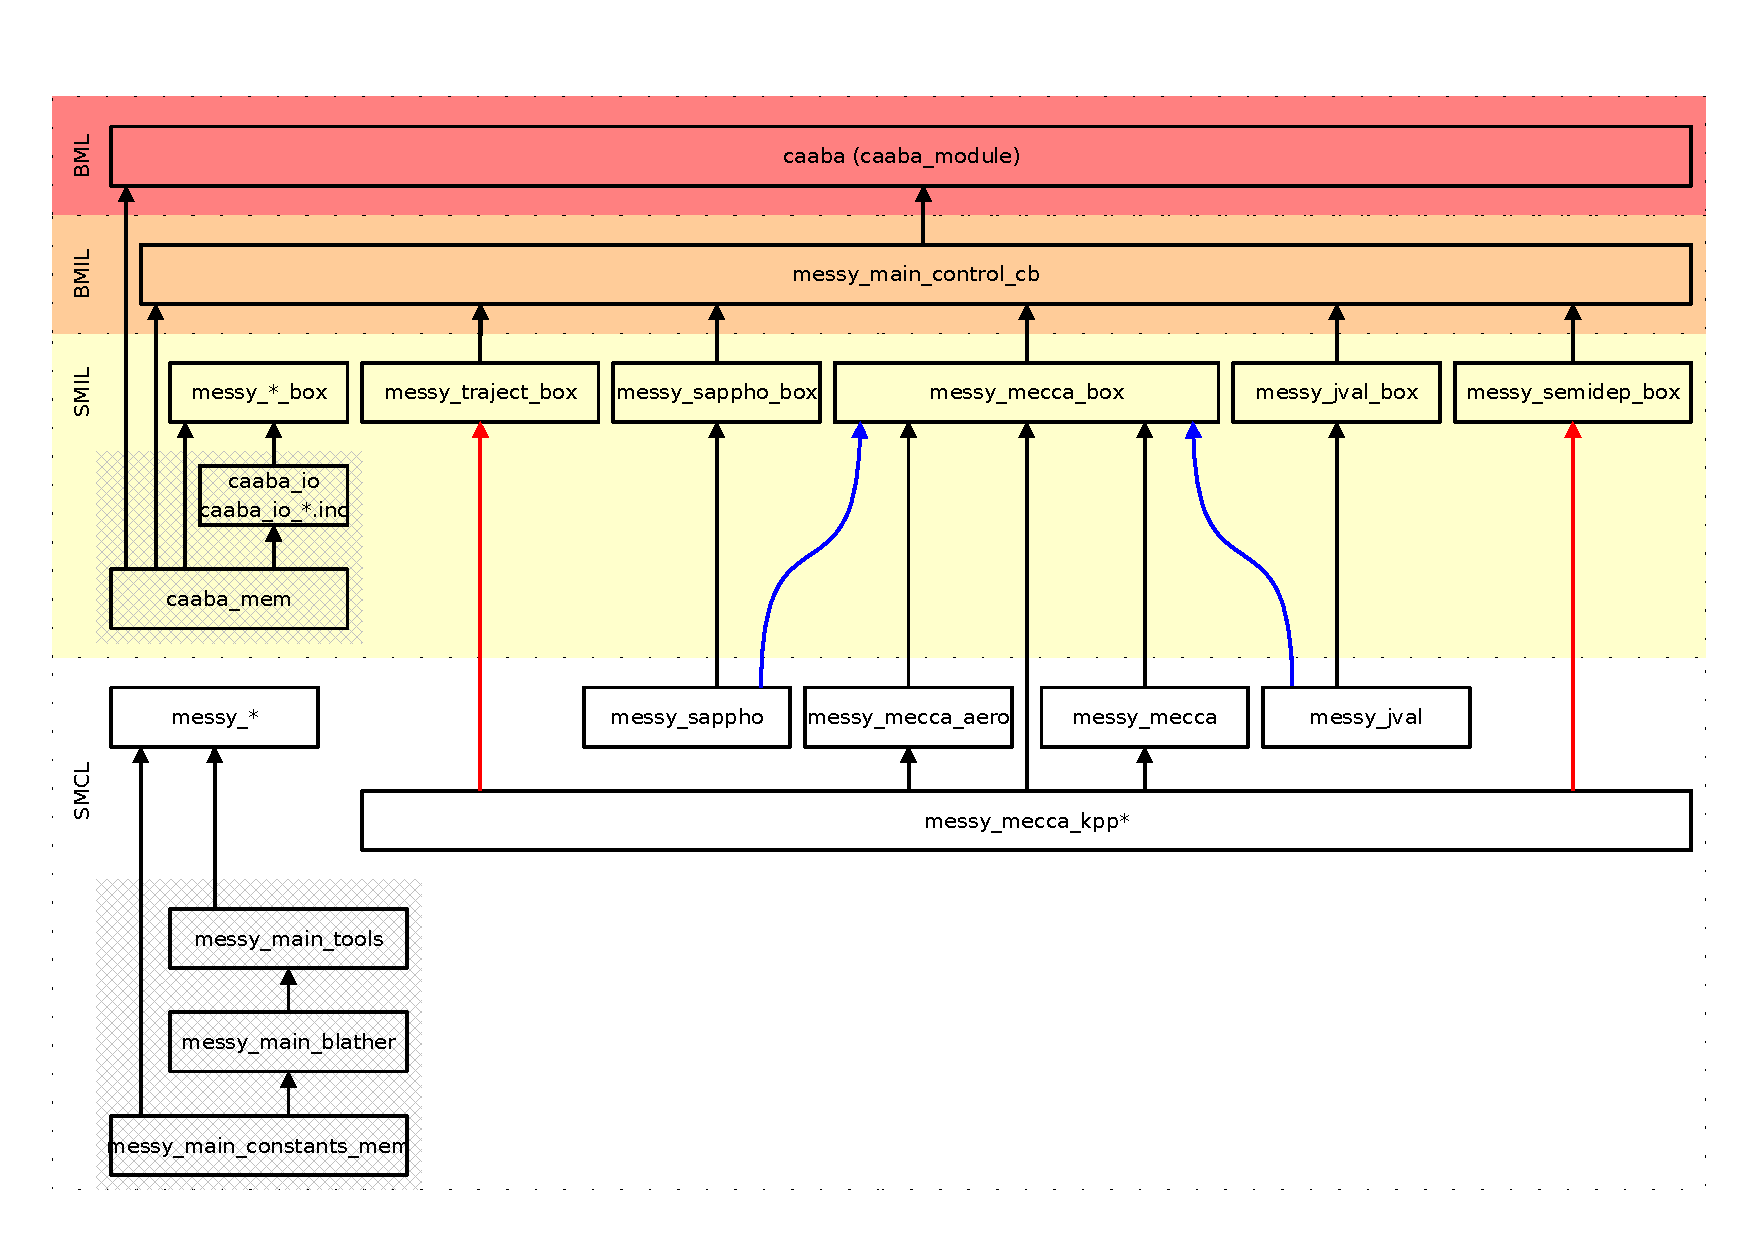
\includegraphics[width=\textwidth]{caaba_use_diagr}
  \end{center}
  \caption{Module structure of \IT{MECCA} when it is connected to the
    \IT{CAABA} \IT{box model}. The box-model related files are in the
    colored layers marked with \IT{BML}, \IT{BMIL}, and \IT{SMIL}. The
    arrows start at the module which is exporting the variables and
    subroutines. They point to the module importing them via the
    \IT{Fortran95} USE instruction. Here, the box {\tt
      messy\_mecca\_kpp*} represents all \I{Kinetic
      PreProcessor}KPP-generated files. The KPP-internal structure is
    shown in Fig.~\ref{fig:kpp_use_diagr}.}
  \label{fig:caaba_use_diagr}
\end{figure*}

\subsection{How to add a new \IT{MESSy} \IT{submodel}}

Below you can find a brief description how to add a new \IT{MESSy}
\IT{submodel}. For more detailed information about programming in the
\IT{MESSy} system, please refer to \citet{2400}.

\begin{itemize}
\item Choose a name (up to 7 lowercase \IT{alphanumerical}
  characters, starting with a letter). Here, ``\verb|xyz|'' is used as
  an example\I{USE\_XYZ}.
\item \verb|caaba_mem.f90|:\\
  \verb|LOGICAL :: USE_XYZ = .FALSE.|
\item \verb|messy_xyz.f90|:\\
  Put all generic subroutines here, i.e.\ all subroutines that are used
  for the \IT{CAABA} boxmodel as well as for a global model.
\item \verb|messy_xyz_box.f90|:\\
  Put \IT{CAABA}-specific code here. Generic code is not included
  directly here. Instead, the generic subroutines in
  \verb|messy_xyz.f90| are called from here. This file contains up to
  four subroutines:
  \begin{itemize}
  \item If the \IT{submodel} needs an \IT{initialization},
    put subroutine \verb|xyz_init| here.
  \item If the \IT{submodel} performs calculations during the
    \IT{time} loop, put subroutine \verb|xyz_physc| here.
  \item If the \IT{submodel} prints results to the screen or
    \IT{netCDF} files, put subroutine \verb|xyz_result| here.
  \item If the \IT{submodel} needs to close any open files at the
    end of the model simulation, put subroutine \verb|xyz_finish| here.
  \end{itemize}
\item \verb|messy_main_control_cb.f90|:
  \begin{itemize}
  \item Add \I{USE\_XYZ}``\verb|USE_XYZ|'' to ``\verb|USE caaba_mem|''.
  \item If subroutine \verb|xyz_init| exists, add:\\
    \verb|USE messy_xyz_box, ONLY: xyz_init|\\
    \verb|IF (USE_XYZ) CALL xyz_init|\\
    to subroutine \verb|messy_init|.
  \item If subroutine \verb|xyz_physc| exists, add:\\
    \verb|USE messy_xyz_box, ONLY: xyz_physc|\\
    \verb|IF (USE_XYZ) CALL xyz_physc|\\
    to subroutine \verb|messy_physc|.
  \item If subroutine \verb|xyz_result| exists, add:\\
    \verb|USE messy_xyz_box, ONLY: xyz_result|\\
    \verb|IF (USE_XYZ) CALL xyz_result|\\
    to subroutine \verb|messy_result|.
  \item If subroutine \verb|xyz_finish| exists, add:\\
    \verb|USE messy_xyz_box, ONLY: xyz_finish|\\
    \verb|IF (USE_XYZ) CALL xyz_finish|\\
    to subroutine \verb|messy_finish|.
  \end{itemize}
\item \verb|caaba_module.f90|:\\
  Edit subroutine \verb|caaba_read_nml|:
  \begin{itemize}
  \item Add \I{USE\_XYZ}``\verb|USE_XYZ|'' to ``\verb|USE caaba_mem|''.
  \item Add ``\verb|USE_XYZ|'' to \IT{namelist} \verb|/CAABA/|.
  \item Print value of \verb|USE_XYZ| (see ``selected \IT{MESSy}
    \IT{submodel}s'').
  \item If applicable, perform consistency checks for interaction of new
    \IT{submodel} with other \IT{submodel}s.
  \end{itemize}
\item \verb|xyz.nml|:\\
  Add sensible default values for controlling the new
  \IT{submodel} (optional).
\item \verb|caaba.nml|:\\
  To activate the new submodel in a CAABA namelist file
  \verb|nml/caaba_*.nml|, add ``\verb|USE_XYZ = T|'' here.
\item \verb|manual/caaba_mecca_manual.tex|:\\
  Mention new \IT{submodel} in this user manual
  (Sections~\ref{sec:submodels} and \ref{sec:f95files},
  Tab.~\ref{tab:files}, and Fig.~\ref{fig:caaba_flowcontrol}).
\end{itemize}

\subsection{General programming guidelines}
\label{sec:guidelines}

To achieve some consistency of the model code, the following guidelines
should be adhered to when writing new code for the \IT{CAABA/MECCA}
modeling system:

\begin{itemize}
\item All Fortran code must be compatible with the \IT{Fortran95}
  standard. \I{compiler}Compiler-specific extensions should not be used.
\item Python-3.6 is the preferred language for new scripts. For shell
  scripts, the \IT{tcsh} is recommended unless there is a specific
  reason for using \IT{bash}, \IT{ksh}, or any other shell.
\item The file names of shell scripts should start with the letter
  \verb|x| for all scripts that are executed directly by the model user.
\item The file names of shell scripts should start with the underscore
  character (``\verb|_|'') if the script is called via another script
  but not executed directly be the user.
\item The names of temporary files should start with the prefix
  \verb|tmp_|.
\end{itemize}

\section{The photolysis submodel \IT{JVAL} and its preprocessor \IT{JVPP}}
\label{sec:jval}

The \IT{JVAL} submodel provides first-order photolysis rate constants
($j$-values) for MECCA. To obtain the \IT{JVAL} parameters for new
photolysis reactions, several calculations are necessary based on UV/VIS
spectra, quantum yields, and their temperature and pressure
dependencies. The JVal PreProcessor (\IT{JVPP}) was written to automate
this process.

\subsection{\IT{JVAL}}

\citet{906} presented an efficient method for online calculations of
photolysis and heating rates which is based on parameterizations in 8
wavelength bands. This method is implemented in the \IT{JVAL} submodel.
The structure of JVAL is shown in Fig.~\ref{fig:calltree_jval}. Note
that for historical reasons, there are two variables for ozone in the
code: \code{relo3_2d} and \code{v3_2d}. Only \code{v3_2d} is used to
calculate $j$-values. The variable \code{relo3_2d} is used to calculate
heating rates (not discussed here). The file \verb|jval.nml| contains
the control namelist \verb|&CTRL|:

\begin{description}
\item[\tt r\_sol:] For the solar cycle, a value of 0 defines the solar
  minimum, and a value of 1 the solar maximum.
\item[\tt qy\_ch3coch3:] There are three options to calculate the
  quantum yield for acetone (\chem{CH_3COCH_3}) photolysis, based on
  different publications. For details, see
  \code{jvpp/dat_lit/hardcoded/jval_cal_CH3COCH3.f90}.
\end{description}

Normally, there is no need to change the default settings of the
namelists.

\begin{table}
  \begin{center}
    \caption{Subdivision of the spectral range into 8 bands.
      $\lambda_{\rm ini}$ and $\lambda_{\rm fin}$ are the initial and
      final wavelength. $\lambda_i$ is a fixed wavelength inside each
      interval. Note that, for historical reasons, the bands are
      numbered from 0 to 7 in the \IT{JVAL} code but 1 to 8 everywhere else.}
    \label{tab:eightbands}
    \begin{tabular}{lccccc}
      \middlehline
      number: name & 
      $\DS\frac{\lambda_{\rm ini}}{\mbox{nm}}$ & 
      $\DS\frac{\lambda_{\rm fin}}{\mbox{nm}}$ &
      $\DS\frac{\lambda_i}{\mbox{nm}}$\\
      \middlehline
      1: Schumann-Runge & 178.555 & 202.030 & \\
      2: Herzberg       & 202.030 & 240.970 & 205.1\\
      3: Hartley        & 240.970 & 289.870 & 287.9\\
      4:                & 289.870 & 305.500 & 302.0\\
      5: UV-B           & 305.500 & 313.500 & 309.0\\
      6:                & 313.500 & 337.500 & 320.0\\
      7: UV-A           & 337.500 & 422.500 & 370.0\\
      8: Chappuis       & 422.500 & 682.500 & 580.0\\
      \bottomhline
    \end{tabular}
  \end{center}
\end{table}

\begin{figure*}[tbh]
  \framebox[\textwidth]{\begin{minipage}{0.9\textwidth}\dirtree{%
  .1 \code{MODULE messy_jval_box}.
     .2 \code{jval_init}\DTcomment{intialization}.
        .3 \code{jval_read_nml_ctrl}\DTcomment{read {\tt\&CTRL} namelist}.
        .3 \code{aerosol_data}\DTcomment{initialize aerosol optical data \citep{2638}}.
        .3 \code{photo_*}\DTcomment{define selected vertical profile ($T$, ozone etc.)}.
     .2 \code{jval_physc}\DTcomment{main calculation}.
        .3 \code{jval_solar_time_control}\DTcomment{set solar cycle parameters}.
        .3 \code{jvalues}\DTcomment{calculate $j$-values}.
           .4 \code{column_cal}\DTcomment{calculate \chem{O_2} and
              \chem{O_3} column densities}.
           .4 \code{flux_cal}\DTcomment{calculate actinic fluxes}.
              .5 \code{slingo}\DTcomment{cloud particle radiative
                 properties \citep{2637}}.
              .5 \code{aero_2d}\DTcomment{apply humidity to aerosol data}.
              .5 \code{pifm}\DTcomment{practical improved flux method}.
                 .6 \code{pifmini}\DTcomment{pifm initialization}.
           .4 \code{jval_cal_uv}\DTcomment{calculate UV radiation}.
           .4 \code{jval_cal}\DTcomment{calculate all $j$-values in inc file}.
              .5 \code{jval_cal_*}\DTcomment{individual subroutines for
                 all species}.
     .2 \code{jval_result}\DTcomment{print results}.
     .2 \code{jval_finish}\DTcomment{deallocate memory of arrays}.
  }\end{minipage}}
  \caption{Call tree of the \IT{JVAL} submodel.}
  \label{fig:calltree_jval}
\end{figure*}

\begin{figure*}[tbh]
  \begin{center}
  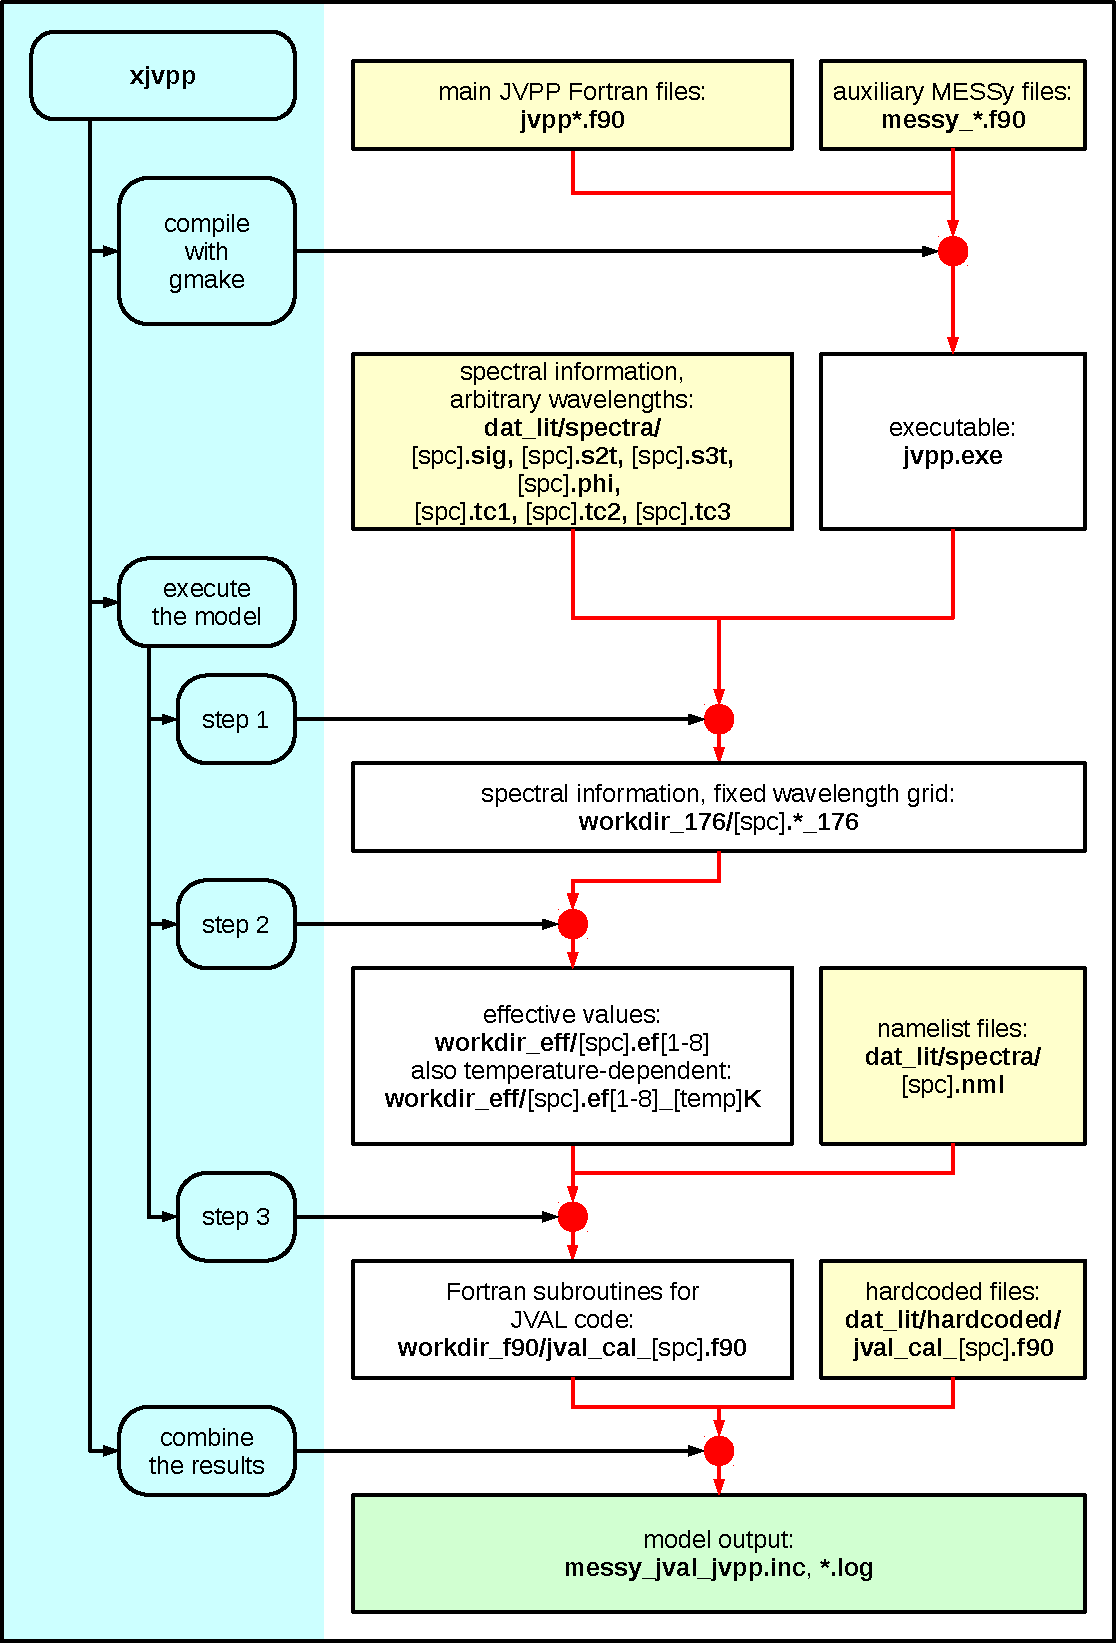
\includegraphics[width=0.84\textwidth]{flowcontrol_xjvpp}
  \end{center}
  \caption{Illustration of the tasks performed by {\tt xjvpp}. {\tt
      xjvpp} and all scripts called by {\tt xjvpp} are shown on a blue
    background. User-generated (static) input files are shown on a
    yellow background whereas automatically generated temporary files
    are shown on a white background.}
  \label{fig:flowcontrol_xjvpp}
\end{figure*}

\begin{table*}[tbh]
  \begin{center}
    \caption{List of \IT{JVPP} files}
    \label{tab:files_jvpp}
    \begin{tabular}{lp{0.55\textwidth}}
      \hline
      \multicolumn{2}{l}{\bf Fortran90 code}\\
      \hline
      \verb|jvpp.f90|                      & main program\\
      \verb|jvpp_step1.f90|                & step 1 (see text)\\
      \verb|jvpp_step2.f90|                & step 2 (see text)\\
      \verb|jvpp_step3.f90|                & step 3 (see text)\\
      \verb|jvpp_mem.f90|                  & common variable declarations\\
      \verb|messy_cmn_photol_mem.f90|      & common definitions shared by different photolysis codes\\
      \verb|messy_main_constants_mem.f90|  & physical constants\\
      \verb|messy_main_math_lsq.f90|       & least-square fit methods\\
      \verb|messy_main_math_spline.f90|    & spline methods\\
      \hline
      \multicolumn{2}{l}{\bf Input}\\
      \hline
      \verb|cheb_coeff.txt|                & Chebyshev coefficients (for \chem{O_2} cross sections)\\
      \verb|jvpp.nml|                      & automatically created namelist file\\
      \verb|dat_lit/|                      & data from recent literature\\
      \verb|dat_lit/spectra/*.nml|         & individual namelist files\\
      \verb|dat_lit/spectra/*.sig|         & original spectra, as from the literature\\
      \verb|dat_lit/spectra/*.s2t|         & spectra at 2 temperatures\\
      \verb|dat_lit/spectra/*.s3t|         & spectra at 3 temperatures\\
      \verb|dat_lit/spectra/*.tc1|         & temperature coefficients (linear)\\
      \verb|dat_lit/spectra/*.tc2|         & temperature coefficients (quadratic)\\
      \verb|dat_lit/spectra/*.phi|         & quantum yields\\
      \verb|dat_lit/hardcoded/*.f90|       & hardcoded subroutines for \IT{JVAL}\\
      \hline
      \multicolumn{2}{l}{\bf Output}\\
      \hline
      \verb|workdir_176/*|                 & temporary data created in step1\\
      \verb|workdir_eff/*|                 & temporary data created in step2\\
      \verb|workdir_f90/*|                 & temporary f90 subroutines for \IT{JVAL}
                                             created in step 3\\
      \verb|workdir_jnl/*|                 & \code{*.jnl} files for plotting the spectra 
                                             and \IT{JVAL} coefficients for the 8 bands\\
      \verb|dat_lit/old/|                  & backup from last run\\
      \verb|references_jvpp.tex|           & sources for the spectra\\
      \hline
      \multicolumn{2}{l}{\bf Other}\\
      \hline
      \verb|xjvpp|                         & tcsh script to execute \IT{JVPP}\\
      \verb|jvpp_plot_step1.py|            & python file for plotting
                                             results of step 1\\
     \hline
    \end{tabular}
  \end{center}
\end{table*}

\begin{figure*}[tbh]
  \framebox[\textwidth]{\begin{minipage}{0.9\textwidth}\dirtree{%
  .1 \code{PROGRAM jvpp}.
     .2 {\bf STEP 1:} \code{conv_sig_176}\DTcomment{interpolate to 176 intervals}.
        .3 \code{process_species}\DTcomment{one call per species}.
           .4 \code{spline_*}\DTcomment{integration or spline}.
     .2 {\bf STEP 2:} \code{conv_176_eff}\DTcomment{calculate effective values}.
        .3 \code{initialize}\DTcomment{initialization}.
           .4 \code{read_tc}\DTcomment{read temperature coefficients}.
           .4 \code{read_phi}\DTcomment{read quantum yields $\varphi$}.
        .3 \code{calc_interval}\DTcomment{loop over bins and temperatures}.
           .4 \code{calc_tdep}\DTcomment{calculate temperature-dependent
              cross sections}.
              .5 \code{sr_o2_km}\DTcomment{parameterization for Schumann-Runge}.
           .4 \code{calc_phi}\DTcomment{calculate quantum yields}.
           .4 \code{sig_eff}\DTcomment{calculate effective values}.
              .5 \code{write_XYZ}\DTcomment{write effective values}.
     .2 {\bf STEP 3:} \code{conv_eff_poly}\DTcomment{polynomial fits}.
        .3 \code{read_nml}\DTcomment{read namelist for each species}.
        .3 \code{process_species}\DTcomment{process each species}.
           .4 \code{process_interval_*}\DTcomment{process each interval
              (constant temperature)}.
              .5 \code{read_file_*d}\DTcomment{read effective values}.
              .5 \code{poly_fit}\DTcomment{polynomial fit}.
           .4 \code{process_tdep_interval_*}\DTcomment{process each
              interval (temperature dependent)}.
              .5 \code{read_file_*d}\DTcomment{read effective values}.
              .5 \code{poly_fit}\DTcomment{polynomial fit}.
           .4 \code{write_*}\DTcomment{write Fortran90 include file for \IT{JVAL}}.
  }\end{minipage}}
  \caption{Main subroutines in the call tree of \IT{JVPP}.}
  \label{fig:calltree_jvpp}
\end{figure*}

\subsection{\IT{JVPP}}
\label{sec:xjvpp}

The file \verb|messy_jval_jvpp.inc|, which is included into
\verb|messy_jval.f90|, contains the Fortran90 subroutines
\verb|jval_cal_*| for all photolysis reactions. To add a new photolysis
reaction to JVAL, a new version of this include file must be created
with the JVal PreProcessor \IT{JVPP}.

\subsubsection{Compiling and running \IT{JVPP} with the shell script
  {\tt xjvpp}}

First, go to the base directory of the \IT{JVPP} code:
\begin{verbatim}
cd tools/jvpp
\end{verbatim}
Note that all path names given in this section are relative to this base
directory. Check that all settings in \verb|Makefile| are correct for
the Fortran90 compiler on your system. Next, the tcsh script
\verb|xjvpp| will guide you through the process of running the code, as
illustrated in Fig.~\ref{fig:flowcontrol_xjvpp}. To execute the script,
type:
\begin{verbatim}
./xjvpp
\end{verbatim}
\verb|xjvpp| will ask several questions, and recommended answers are
given below. If you only press the Return key, you select the default.
\begin{verbatim}
Compile f90 files?
[y|n|q, default=y]
\end{verbatim}
Choose ``\verb|y|'' to compile the Fortran90 files and create the
executable \verb|jvpp.exe|. The input directory ``\verb|dat_lit/|''
contains the most recent UV/VIS data from the literature.
\begin{verbatim}
Clean-up workdir and run jvpp.exe?
[y|n|q, default=y]
\end{verbatim}
Unless there were any errors, choose ``\verb|y|'' now to remove
temporary files from the working directory and to start the \IT{JVPP}
executable. After \verb|jvpp.exe| has finished, the screen output can
also be found in \verb|jvpp.log|. More detailed information is available
from \verb|jvpp_detail.log|.

\begin{table*}[tbh]
  \begin{center}
    \renewcommand{\arraystretch}{1.05}
    \caption{Wavelengths (in nm) of the fixed grid created in step 1 of
      \IT{JVPP}. The full grid contains 176 wavelengths. However, here only
      the first 142 wavelengths are shown here because those above
      680~nm are currently not used.}
    \label{tab:wave176}
    \small
    \begin{tabular}{|rp{0.15\textwidth}|rp{0.15\textwidth}|rp{0.15\textwidth}|}
      \bottomhline
      \multicolumn{2}{|l|}{\bf 1) Schumann-Runge} & \multicolumn{2}{|l|}{\bf 4)}      & \multicolumn{2}{|l|}{\bf 8) Chappuis} \\\hline
        1 & 179.37                                &  44 & 291.97                      &  91 & 425.00                          \\
        2 & 181.00                                &  45 & 296.30                      &  92 & 430.00                          \\
        3 & 182.65                                &  46 & 299.00                      &  93 & 435.00                          \\
        4 & 184.33                                &  47 & 300.00                      &  94 & 440.00                          \\
        5 & 186.05                                &  48 & 301.00                      &  95 & 445.00                          \\
        6 & 187.79                                &  49 & 302.00                      &  96 & 450.00                          \\
        7 & 189.57                                &  50 & 303.00                      &  97 & 455.00                          \\
        8 & 191.39                                &  51 & 304.00                      &  98 & 460.00                          \\
        9 & 193.24                                &  52 & 305.00                      &  99 & 465.00                          \\\cline{3-4}
       10 & 195.12                                & \multicolumn{2}{|l|}{\bf 5) UV-B} & 100 & 470.00                          \\\cline{3-4}
       11 & 197.04                                &  53 & 306.00                      & 101 & 475.00                          \\
       12 & 199.00                                &  54 & 307.00                      & 102 & 480.00                          \\
       13 & 201.01                                &  55 & 308.00                      & 103 & 485.00                          \\\cline{1-2}
      \multicolumn{2}{|l|}{\bf 2) Herzberg}       &  56 & 309.00                      & 104 & 490.00                          \\\cline{1-2}
       14 & 203.05                                &  57 & 310.00                      & 105 & 495.00                          \\
       15 & 205.13                                &  58 & 311.00                      & 106 & 500.00                          \\
       16 & 207.25                                &  59 & 312.00                      & 107 & 505.00                          \\
       17 & 209.42                                &  60 & 313.00                      & 108 & 510.00                          \\\cline{3-4}
       18 & 211.64                                & \multicolumn{2}{|l|}{\bf 6)}      & 109 & 515.00                          \\\cline{3-4}
       19 & 213.90                                &  61 & 314.00                      & 110 & 520.00                          \\
       20 & 216.22                                &  62 & 315.00                      & 111 & 525.00                          \\
       21 & 218.58                                &  63 & 316.00                      & 112 & 530.00                          \\
       22 & 220.99                                &  64 & 317.00                      & 113 & 535.00                          \\
       23 & 223.46                                &  65 & 318.00                      & 114 & 540.00                          \\
       24 & 225.99                                &  66 & 319.00                      & 115 & 545.00                          \\
       25 & 228.57                                &  67 & 320.00                      & 116 & 550.00                          \\
       26 & 231.21                                &  68 & 321.00                      & 117 & 555.00                          \\
       27 & 233.92                                &  69 & 322.50                      & 118 & 560.00                          \\
       28 & 236.69                                &  70 & 324.50                      & 119 & 565.00                          \\
       29 & 239.52                                &  71 & 326.50                      & 120 & 570.00                          \\\cline{1-2}
      \multicolumn{2}{|l|}{\bf 3) Hartley}        &  72 & 330.00                      & 121 & 575.00                          \\\cline{1-2}
       30 & 242.42                                &  73 & 335.00                      & 122 & 580.00                          \\\cline{3-4}
       31 & 245.40                                & \multicolumn{2}{|l|}{\bf 7) UV-A} & 123 & 585.00                          \\\cline{3-4}
       32 & 248.45                                &  74 & 340.00                      & 124 & 590.00                          \\
       33 & 251.57                                &  75 & 345.00                      & 125 & 595.00                          \\
       34 & 254.78                                &  76 & 350.00                      & 126 & 600.00                          \\
       35 & 258.06                                &  77 & 355.00                      & 127 & 605.00                          \\
       36 & 261.44                                &  78 & 360.00                      & 128 & 610.00                          \\
       37 & 264.90                                &  79 & 365.00                      & 129 & 615.00                          \\
       38 & 268.46                                &  80 & 370.00                      & 130 & 620.00                          \\
       39 & 272.11                                &  81 & 375.00                      & 131 & 625.00                          \\
       40 & 275.86                                &  82 & 380.00                      & 132 & 630.00                          \\
       41 & 279.72                                &  83 & 385.00                      & 133 & 635.00                          \\
       42 & 283.69                                &  84 & 390.00                      & 134 & 640.00                          \\
       43 & 287.77                                &  85 & 395.00                      & 135 & 645.00                          \\\cline{1-2}
          &                                       &  86 & 400.00                      & 136 & 650.00                          \\
          &                                       &  87 & 405.00                      & 137 & 655.00                          \\
          &                                       &  88 & 410.00                      & 138 & 660.00                          \\
          &                                       &  89 & 415.00                      & 139 & 665.00                          \\
          &                                       &  90 & 420.00                      & 140 & 670.00                          \\\cline{3-4}
          &                                       &     &                             & 141 & 675.00                          \\
          &                                       &     &                             & 142 & 680.00                          \\
      \hline
    \end{tabular}\\[1cm]
  \end{center}
\end{table*}

The \IT{JVPP} code consists of the files listed in Tab.~\ref{tab:files_jvpp}.
The main program \verb|jvpp.f90| works in three steps as described below
and shown in Fig.~\ref{fig:calltree_jvpp}.

\subsubsection{Step 1 of \IT{JVPP}}

The file \verb|jvpp_step1.f90| contains the code to perform the first
step. Here, the subroutine \code{conv_sig_176} converts (interpolates)
cross sections $\sigma$ from literature data to the 176 fixed
wavelengths shown in Table~\ref{tab:wave176}. The code loops over all
photolysis reactions (from 1 to \code{IP_MAX}). For each reaction, it is
checked if there are any input files for the spectra (cross sections),
their quantum yields, and/or their temperature dependencies. Files with
the following extensions can be used as model input:

\begin{description}
\item [\code{*.sig}:] temperature-independent spectrum
\item [\code{*.s2t}:] 2 spectra at 2 temperatures
\item [\code{*.s3t}:] 3 spectra at 3 temperatures
\item [\code{*.phi}:] quantum yields (between 0 and 1)
\item [\code{*.tc1}:] linear temperature coefficients (1st order
  polynomial)
\item [\code{*.tc2}:] quadratic temperature coefficients (2nd order
  polynomial)
\item [\code{*.tc3}:] cubic temperature coefficients (3rd order
  polynomial)
\end{description}

The input files start with an arbitrary number of header lines which
must begin with the character ``\code{#}''. The following lines must
contain data. The first column defines the wavelength in \unit{nm}. The
content of the following columns depends on the file type. For the
\code{*.sig} files, the second column contains (temperature-independent)
cross sections in \unit{cm^2}. The temperature-dependent files contain
additional lines and columns.

The data from each of these files is interpolated to the 176 fixed
wavelengths. The default interpolation method is integration
(\code{spline_method} = \code{integration}). It performs a linear
interpolation between the points of the original spectrum and conserves
the integrated value. As an alternative, it is possible to select other
methods, based on code from John Burkardt
(\url{https://people.sc.fsu.edu/~jburkardt/f_src/spline/spline.html}): A
linear spline method (\code{linear_val}), a cubic B spline
(\code{b_val}), a piecewise constant spline (\code{constant_val}), and a
piecewise quadratic spline method (\code{quadratic_val}) are available.

The results are written to temporary files with the suffix
``\verb|.*_176|'' in the directory \verb|workdir_176/|.

\subsubsection{Step 2 of \IT{JVPP}}

The file \verb|jvpp_step2.f90| contains the code to perform the second
step. Here, the subroutine \code{conv_176_eff} reads data for the 176
bins from \verb|workdir_176/| and then converts them to effective values
for the eight bands shown in Table~\ref{tab:eightbands}. First, output
from step 1 is read in:
\begin{itemize}
\item If there are any temperature-dependent (\code{*.s2t} or
  \code{*.s3t}) or temperature-independent (\code{*.sig}) cross-section
  input files, the data is read into the variables \code{cs_XYZ_tdep} or
  \code{cs_XYZ}, respectively.
\item If there are any files containing temperature coefficients
  (\code{*.tc1}, \code{*.tc2}, or \code{*.tc3}), the data is read into
  the variable \code{tc_XYZ}.
\item If there are any files containing quantum yields (\code{*.phi}),
  the data is read into the variable \code{phi_XYZ}.
\end{itemize}
Next, the code loops over all bands (from 1 to 8), first for
calculations at a fixed reference temperature (240~\unit{K} for interval
1 and 250~\unit{K} for intervals 2-8), then for calculations at several
temperatures (from 180~\unit{K} to 320~\unit{K}). For each band:
\begin{itemize}\nosep
\item Temperature-dependent cross sections \code{cst_XYZ} are calculated
  in subroutine \code{calc_tdep}:
  \begin{itemize}\nosep
  \item via \code{cs_XYZ_tdep} from \code{*.s2t} or \code{*.s3t} files
  \item via temperature coefficients \code{tc_XYZ} from \code{*.tc1},
    \code{*.tc2}, or \code{*.tc3} files
  \item via individual wavelength-dependent functions defined in the
    code
  \end{itemize}
\item Quantum yields are calculated in subroutine \code{calc_phi}.
\item Effective values are calculated in subroutine \code{sig_eff}:
  \begin{itemize}\nosep
  \item Ozone columns and optical depths \code{tau_o3} are defined.
  \item Oxygen columns and optical depths \code{tau_o2} are defined.
  \item The code loops over all \chem{O_3} and \chem{O_2} columns and
    calculates intermediate values for all photolysis reactions.
  \end{itemize}
\end{itemize}

The resulting effective values are written to temporary files in the
directory \verb|workdir_eff/|. The suffix of these files is
``\verb|.ef|[{\em 1-8}\/]'' for temperature-independent data and
``\verb|.ef|[{\em 1-8}\/]\verb|_|[{\em temp}\/]\verb|K|'' for
temperature-dependent data. Here [{\em 1-8}\/] denotes the wavelength
band between 1 and 8 and [{\em temp}\/] is the temperature.

\subsubsection{Step 3 of \IT{JVPP}}

The file \verb|jvpp_step3.f90| contains the code to perform the third
step. First, the subroutine \code{conv_eff_poly} looks for namelist
files. For all species with a namelist, the subroutine
\code{process_species} is called. It reads the effective values from
\verb|workdir_eff/| and then finds polynomial fits for them. From the
parameterization, the Fortran90 code of \verb|SUBROUTINE jval_cal_XYZ|
is generated, where \verb|XYZ| is the name of the species.

Finally, the script \verb|cat_jval.tcsh| (also created by
\verb|jvpp_step3.f90|) is used to concatenate all individual subroutines
\verb|jval_cal_*| into the include file \verb|messy_jval_jvpp.inc|.

\subsubsection{Namelist control}
\label{sec:nml}

The main namelist file \verb|jvpp.nml| is created automatically by
\verb|xjvpp| and should not be edited manually.

In contrast, the individual namelist files for each photolysis reaction
can be changed manually. They are in the same input directory as the
spectra: \verb|dat_lit/spectra/|. They contain the \verb|JVPP| namelist
which is used in step 3. The entries are:
\begin{itemize}\nosep
\item The degree of the fitting functions for temperature-independent
  and temperature-dependent effective values can be defined with
  \verb|deg_tconst| and \verb|deg_tdep|, respectively. Each of the 8
  bands can have individual values. The default is:\\
  \verb|deg_tconst| = (/ 1, 1, 1, 1, 3, 3, 3, 3 /)\\
  \verb|deg_tdep  | = (/ 2, 2, 2, 2, 2, 2, 2, 2 /)
\item Eight correction factors $F_{corr}$, based on eight values of
  $b_i$, are available for zenith angles above 87.5\degree, as shown in
  Fig.~\ref{fig:lamago}. The parameter \verb|fj_corr| is used to select
  a suitable value of $b_i$ based on the wavelength region in which the
  species absorbs, according to Table 1 of \citet{2642}. If the factor
  is not defined in the namelist, the default value \verb|fj_corr| = 7
  is used.
\item If absorption at the Lyman-alpha wavelength (e.g., \chem{CO_2},
  \chem{O_2}) or in the infrared region (e.g., \chem{HNO_4}) is
  important, its contribution can be defined as \verb|lya_ir|.
\item If \IT{JVPP} is unable to calculate the parameters for \IT{JVAL} (e.g.,
  because of density dependence correction for acetone), setting
  \verb|l_hardcoded| to \verb|.TRUE.| will simply use a manually written
  subroutine from \verb|dat_lit/hardcoded/|. Examples can be seen in
  \verb|CH3COCH3.nml|, \verb|GLYOX.nml|, and \verb|NO.nml|.
\end{itemize}
In addition, some metadata should be provided:
\begin{itemize}\nosep
\item \verb|eqntag| is the number of the photolysis reaction in MECCA,
  e.g., \verb|eqntag = "J3101"| for the photolysis of \chem{NO_2}.
\item \verb|texrxn| contains the photolysis reaction in La\TeX\ syntax,
  e.g.: \verb|"NO_2 \TOHV\ NO + O"|.
\item \verb|texnote| provides the Bib\TeX\ key of the reference for the
  spectrum. It may also contain additional information in La\TeX\
  syntax, e.g.: \verb|"Lyman-alpha from Fig. 1 of \cite{2354}"| for
  \chem{CH_4}.
\end{itemize}

\begin{figure}
  \begin{center}
  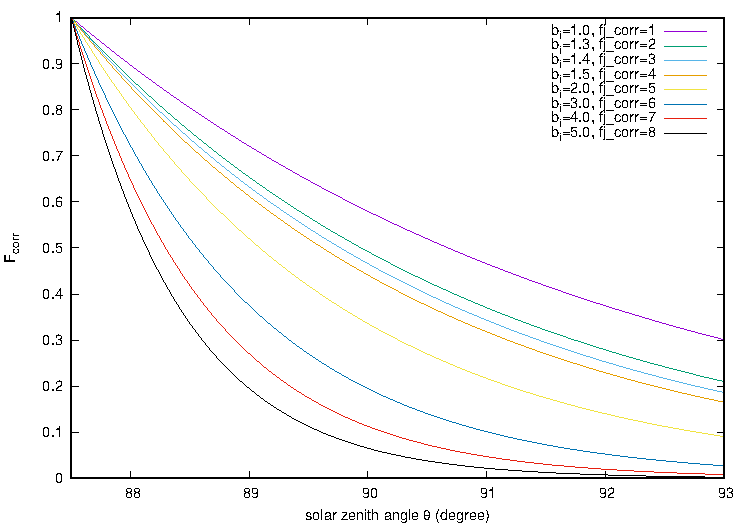
\includegraphics[width=\columnwidth]{lamago}
  \end{center}
  \caption{Correction factor $F_{corr}$ for large solar zenith angles
    $\theta$ calculated as
    $F_{corr}(\theta) = \exp(19.09 \times b_i \times (1-\theta/87.5))$
    according to \citet{2642}.}
  \label{fig:lamago}
\end{figure}

\subsection{Modifying \IT{JVAL} and \IT{JVPP}}

To add the photolysis of a new species (called ``XYZ'' here) to the
code, the following changes are necessary:

\begin{itemize}\nosep
\item Add the photolysis to \code{messy_cmn_photol_mem.f90}:
  \begin{itemize}\nosep
  \item add \code{ip_XYZ}
  \item increase \code{IP_MAX}
  \item add string to \code{jname}
  \end{itemize}
\item Create a new namelist file \code{XYZ.nml} with appropriate values
  and save it in the \code{dat_lit/spectra/} directory:
  \begin{itemize}
  \item define the MECCA equation tag \code{eqntag} (the ``reaction
    number'')
  \item define the reaction \code{texrxn} and a note with a reference
    \code{texnote} in La\TeX\ syntax
  \item if the default is not suitable, define \code{fj_corr} according
    to \citet{2642}
  \item if the default is not suitable, define the degree of the fitting
    functions \code{deg_tconst} and/or \code{deg_tdep}
  \item optionally, define \code{lya_ir} for a Lyman-$\alpha$ or
    infrared contribution
  \end{itemize}
\item Get the UV/VIS spectrum (e.g., from \citet{2872}) and enter it to
  a new file \code{XYZ.sig} in the \code{dat_lit/spectra/} directory.
\item If the cross sections are temperature-dependent, choose one of the
  following options:
  \begin{itemize}\nosep
  \item Create a \verb|XYZ.s2t| or \verb|XYZ.s3t| file if the spectrum
    is known at two or three temperatures, respectively.
  \item Create a \verb|XYZ.tc1|, \verb|XYZ.tc2|, or \verb|XYZ.tc3| file
    if the spectrum can be described with a function containing 1, 2, or
    3 parameters. Add the corresponding function to \verb|SUBROUTINE|
    \verb|calc_tdep| in \verb|jvpp_step2.f90|.
  \item For more complex cases, add an individual wavelength-dependent
    function at the end of \verb|SUBROUTINE| \verb|calc_tdep| in
    \verb|jvpp_step2.f90|.
  \end{itemize}
\item If the quantum yield is not always equal to one, add a
  \verb|XYZ.phi| file to the directory \code{dat_lit/spectra/}.
\item Execute the \IT{JVPP} code via \verb|xjvpp| as described in
  Sect.~\ref{sec:xjvpp}.
\item If the new photolysis reaction is used in the global ECHAM5/MESSy
  Atmospheric Chemistry (EMAC) model \citep{2400}, it is necessary to
  activate its calculation in \verb|messy_jval_si.f90| with:\\
  \verb|IF (TRIM(basename) == 'XYZ') &|
  \verb|  lps(ip_XYZ,j) = .TRUE.|
\end{itemize}

\section{MECCA in the MESSy modeling system}
\label{sec:messy}

Apart from using MECCA inside the CAABA box model, it is also possible
to connect the MECCA chemistry to another \IT{base model} via the MESSy
interface \citep[][\url{http://www.messy-interface.org}]{1664,2400}. For
example, MECCA chemistry is used in many studies with the global,
3-dimensional ECHAM/MESSy Atmospheric Chemistry (EMAC) model
\citep{1851,3068}.

\subsection{Data transfer}

The files of the CAABA/MECCA model can be subdivided into those that are
independent of the CAABA box model (\IT{submodel} core layer, \IT{SMCL})
and those that are specific to the boxmodel (\IT{submodel} interface
layer, \IT{SMIL}). Figure~\ref{fig:caaba_use_diagr} shows SMIL files
with a yellow and SMCL files with a white background. The SMCL files can
be used without any modifications when MECCA is connected to a different
base model. The following variables and subroutines must be transfered
between the SMCL module \verb|messy_mecca_kpp| and the SMIL layer:

\begin{itemize}
\item {\bf \verb|INTEGER NSPEC|:} the number of chemical species
\item {\bf \verb|INTEGER ind_*|:} the KPP-generated indices of the
  chemical species
\item {\bf \verb|SUBROUTINE initialize_kpp_ctrl|:} read the KPP CTRL
  namelist
\item {\bf \verb|SUBROUTINE initialize|:} define the tolerances rtol and
  atol
\item {\bf \verb|SUBROUTINE fill_jx|, \verb|fill_cair|,
    \verb|fill_temp|, \verb|fill_press|:} subroutines that transfer the
  $j$-values \verb|jx|, the concentration of air, temperature and
  pressure
\item {\bf \verb|SUBROUTINE kpp_integrate|:} the main kpp call
\end{itemize}

The script \code{xmecca} also generates 4 include files which are only
needed if MECCA is connected to a MESSy base model that uses the TRACER
infrastructure \citep{2097}, e.g., ECHAM/MESSy. These files assign
chemical species from MECCA to tracers of the basemodel:

\begin{itemize}
\item \verb|messy_mecca_idt_si.inc|: Declares the indices \verb|idt_*|
  of the tracers corresponding to MECCA species.
\item \verb|messy_mecca_c2mr_si.inc|: Converts the concentration of a
  MECCA species to the mixing ratio of a tracer.
\item \verb|messy_mecca_mr2c_si.inc|: Converts the mixing ratio of a
  tracer to the concentration of a MECCA species.
\item \verb|messy_mecca_trac_si.inc|: Defines new tracers corresponding
  to MECCA species.
\end{itemize}

\begin{figure*}
  \begin{center}
    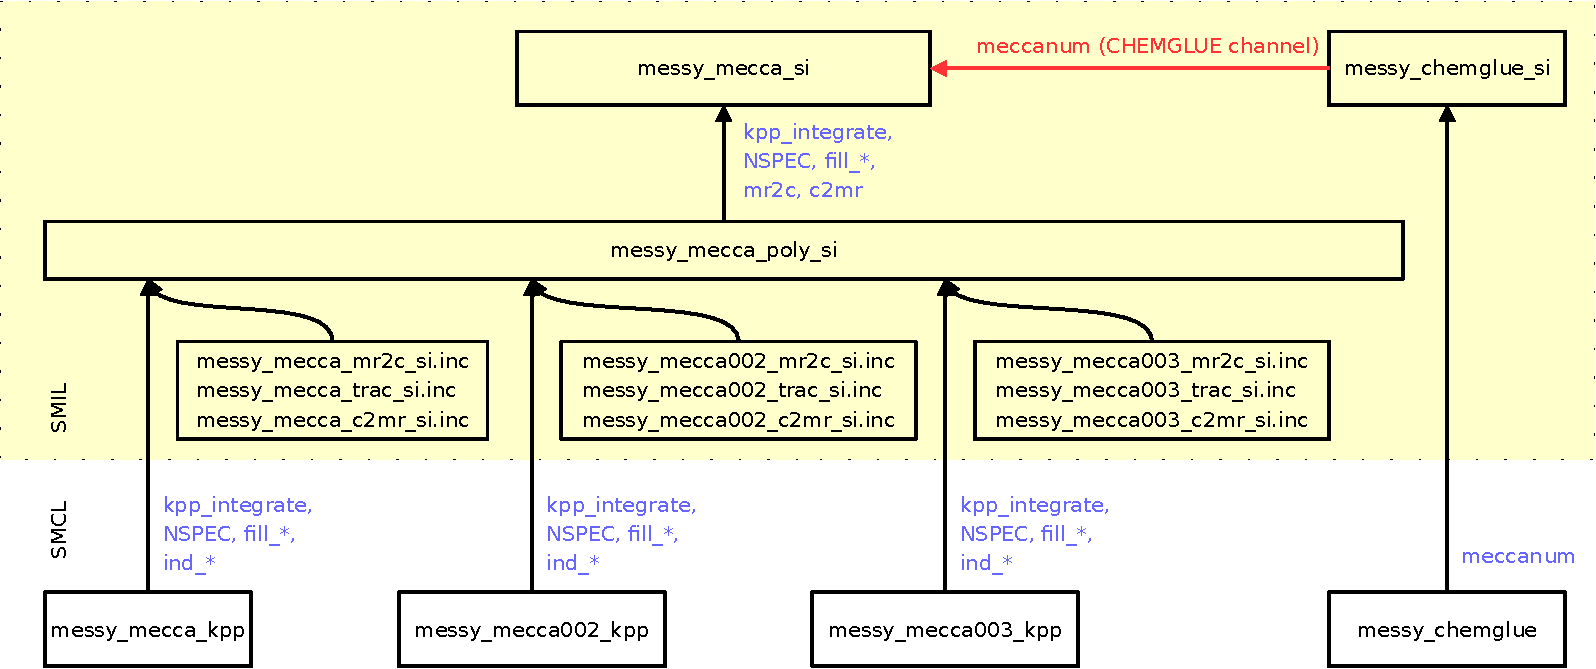
\includegraphics[width=\textwidth]{polymecca_use_diagr}
  \end{center}
  \caption{Module structure of PolyMECCA and CHEMGLUE. The black arrows
    represent the import of the associated blue variables via the
    Fortran95 USE instruction. Red arrows represent data import via a
    MESSy channel.}
  \label{fig:polymeccause}
\end{figure*}

\subsection{\IT{PolyMECCA} and \IT{CHEMGLUE}}
\label{sec:PolyMECCA}

\subsubsection{Usage}

Running ECHAM5/MESSy with two or more different chemical mechanisms:

\begin{enumerate}
\item For each chemical mechanism, select (or create) a MECCA batch
  file. The names of new batch files must be added to the declarations
  in \verb|messy_chemglue.f90| (replacing ``-'' and ``.'' by the
  underscore ``\_''). For testing purposes, the batch file
  \verb|CCMI/CCMI-base-02-polymeccatest.bat| can be used.
\item Edit the file \verb|xpolymecca| (in the \verb|mbm/caaba/mecca/|
  directory) and enter the selected batch files into the definition of
  \verb|$batchfiles|.
\item Execute \verb|xpolymecca|. Now, two or more chemical mechanisms
  are available.
\item Switch on CHEMGLUE in \verb|switch.nml|.
\item Find a suitable subroutine \verb|select_mechanism_from_*| in the
  SMCL file \verb|messy_chemglue.f90| (or create a new one). This
  subroutine decides at runtime in each model time step, which chemical
  mechanism is selected under which conditions.
\item Call the chosen subroutine \verb|select_mechanism_from_*| from
  subroutine \verb|chemglue_physc| in \verb|messy_chemglue_si.f90|,
  providing the necessary input fields.
\item Compile and run the model.
\end{enumerate}

Resetting ECHAM5/MESSy to one chemical mechanism:

\begin{enumerate}
\item Execute xmecca with any batch file, e.g.:
  \verb|./xmecca CCMI/CCMI-base-02|.
\item Switch off CHEMGLUE in \verb|switch.nml|.
\end{enumerate}

\subsubsection{\IT{xpolymecca}}

The main component of PolyMECCA is the script \verb|xpolymecca|, which
calls xmecca several times and produces the core layer (SMCL) files for
all MECCA mechanisms, as well as some include files (\verb|*.inc|) for
the interface layer (SMIL). The first mechanism is simply called
``MECCA'', and subsequent mechanisms are called ``MECCA002'',
``MECCA003'', and so on. Files belonging to mechanisms from previous
executions of \verb|xpolymecca| are deleted. One mechanism is generated
for each entry included in the variable \verb|batchfiles|. If the array
\verb|batchfiles| contains only one element, only one mechanism called
``MECCA'' is generated. Using mechanism number 2 as an example, the
following files are created for the SMCL:
\begin{itemize}
\item \verb|messy_mecca002_kpp.kpp| \hfill (KPP control file)
\item \verb|mecca002.spc|           \hfill (KPP species file)
\item \verb|mecca002.eqn|           \hfill (KPP equation file)
\item \verb|messy_mecca002_kpp.f90| \hfill (main Fortran95 file)
\item \verb|xmecca002.log|          \hfill (xmecca log file)
\item \verb|mecca002nism.pdf|       \hfill (mechanism, optional)
\item \verb|mecca002_*.pdf|         \hfill (graphviz plots, optional)
\item \verb|messy_chemglue.inc|     \hfill (CHEMGLUE SMCL)
\end{itemize}
The following files are created for the SMIL:
\begin{itemize}
\item \verb|messy_mecca002_c2mr_si.inc|
\item \verb|messy_mecca002_idt_si.inc|
\item \verb|messy_mecca002_mr2c_si.inc|
\item \verb|messy_mecca002_trac_si.inc|
\end{itemize}

\subsubsection{The submodel interface layer files messy\_mecca\_si.f90
  and messy\_mecca\_poly\_si.f90}

Before the implementation of PolyMECCA, the SMIL file
\verb|messy_mecca_si.f90| imported the variables and subroutines
\verb|kpp_integrate|, \verb|NSPEC|, \verb|fill_*|, \verb|mr2c| and
\verb|c2mr| directly from the SMCL file \verb|messy_mecca_kpp.f90| via
the Fortran95 \verb|USE| command. Now, this information is collected by
\verb|messy_mecca_poly_si.f90| for all mechanisms (MECCA, MECCA002,
etc.), as shown in Fig.~\ref{fig:polymeccause}. Depending on the number
of the selected mechanism (\verb|meccanum|), appropriate values are
transfered from \verb|messy_mecca_poly_si.f90| to
\verb|messy_mecca_si.f90|.

\subsubsection{Current limitations}

\begin{itemize}
\item The following variables are usually different for each mechanism
  but currently, the diagnostic output only shows data for the first
  mechanism: \verb|IERR_NAMES|, \verb|rplfile|, \verb|wanted|,
  \verb|diagtracfile|, \verb|gas_eqn_file|, \verb|batchfile|.
% \item PolyMECCA does not work for Lagrangian calculations: For
%   Lagrangian calculations, \verb|messy_mecca_si.f90| has its own
%   \verb|mr2c| and \verb|c2mr| subroutines and does not use those
%   provided by \verb|messy_mecca_poly_si.f90|.
\item PolyMECCA has not been tested with tagging.
\item The indices for heterogeneous reactions (\verb|ihs_*|,
  \verb|iht_*|) must be the same for all mechanisms because
  \verb|messy_mecca_khet_si.f90| gets all its values from
  \verb|messy_mecca_kpp.f90| (not from \verb|messy_mecca002_kpp.f90|
  etc.). This is not a problem as long as these values are taken from
  \verb|messy_mecca_kpp.kpp| for all mechanisms.
\item PolyMECCA does not work with \verb|mecca_aero|.
\item PolyMECCA only works with KP4 (\verb|kppoption=4|) but not with
  \verb|kppoption=k|.
\item The same numerical integrator must be used in all mecca batch
  files.
\item The same photolysis submodel must be used for all mechanisms.
\end{itemize}

\subsubsection{CHEMGLUE}
\label{sec:chemglue}

CHEMGLUE creates and defines the channel object \verb|meccanum_gp| based
on the conditions in each box. If this channel object exists,
\verb|messy_mecca_si.f90| chooses the mechanism based on the contents of
\verb|meccanum_gp|. The CHEMGLUE files are:
\begin{itemize}
\item \verb|messy_chemglue.f90| \hfill (SMCL)
\item \verb|messy_chemglue_si.f90| \hfill (SMIL)
\item \verb|messy_chemglue.inc| \hfill (automatically created by
  \verb|xpolymecca|, do not edit manually)
\item messy/nml/DEFAULTS/chemglue.nml \hfill (dummy namelist)
\end{itemize}

\subsubsection{Modifying PolyMECCA and CHEMGLUE}

Adding batch files:

\begin{itemize}
\item Add new batch file to the \verb|mecca/batch/| directory.
\item In \verb|messy/smcl/messy_chemglue.f90|, add a variable
  representing the batch file name (same name but ``.'' and ``-''
  replaced by the underscore ``\_'').
\end{itemize}

Choosing a certain reaction mechanism:

\begin{itemize}
\item Create a new PUBLIC SUBROUTINE called
  \verb|select_mechanism_from_*| and add it to
  \verb|messy_chemglue.f90|.
\item USE and CALL the new subroutine from \verb|chemglue_physc| in
  \verb|messy_chemglue_si.f90|.
\end{itemize}

\bibliographystyle{egu} % bst file
\bibliography{literat}  % bib files

\printindex

\end{document}
